\section{Funcionalidad del cliente}
La capa de cliente se ha implementado teniendo como público objetivo a los usuarios del sistema operativo Android.

El razonamiento detrás de esta decisión reside en los siguientes puntos:
\begin{itemize}
    \item La cuota de mercado del sistema operativo Android a nivel europeo es aproximadamente del 70\%, de modo de la aplicación tiene una base de usuarios potenciales más amplia que cualquier otro sistema operativo para dispositivos móviles \cite{gs_statscounter}.
    \item Tiene código abierto y ofrece mayor libertad al poder desarrollar sin necesidad de pedir permisos.
    \item Android cuenta con un sistema multitarea que permite abrir distintas aplicaciones a la vez y hacerlas funcionar simultáneamente, así como ponerlas en modo suspensión, si no las estamos utilizando.
    \item El sistema de sincronización de Android en la nube demuestra una elevada eficiencia, ya que al estar ligado a Google, los servicios web cuentan con un gran sistema de trabajo.
    \item La aplicación al estar instalada en el dispositivo, se ejecuta mucho más rápido que si tuviera que cargar e interpretar código proveniente de otra fuente.
\end{itemize}

\subsection{Ciclo de vida de una actividad}
Todas las actividades o pantallas visibles de la aplicación, tiene un ciclo de vida similar que pasa por varios estados que pueden verse en la figura \ref{fig:flujo_vida_actividad} .


\begin{figure}[H]
    \centering
    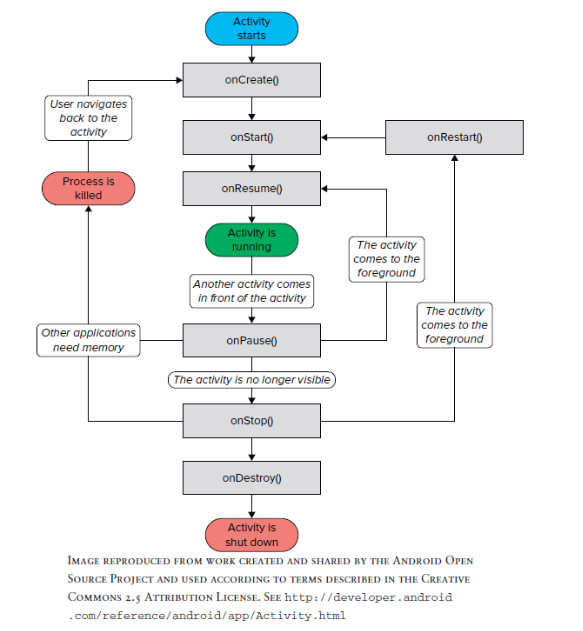
\includegraphics[width=0.8\textwidth]{Images/Capitulo7/flujo_vida_actividad.png}
    \caption{Flujo de vida de una actividad}
    \label{fig:flujo_vida_actividad}
\end{figure}

La actividad se crea en la función \texttt{onCreate()}, esta función es similar en todas las actividades de la aplicación, en la figura \ref{fig:oncreate} se muestra un ejemplo en código de la función.

\begin{figure}[H]
    \centering
    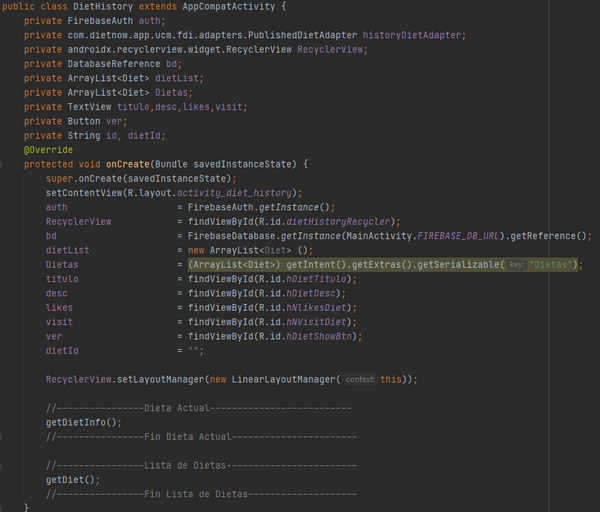
\includegraphics[width=\textwidth]{Images/Capitulo7/oncreate.png}
        \caption{Código de la función \texttt{onCreate()}}
    \label{fig:oncreate}
\end{figure}

La mayoría de las actividades creadas para el desarrollo de la aplicación siguen una serie de pasos: 
\begin{enumerate}
    \item Se establece la vista a la que hace referencia la actividad, en este caso es la se hace referencia a la vista de la figura \ref{fig:dietaview}.
    \item Se inicializan los elementos de la vista, así como la referencia a la base de datos y al módulo de autenticación.
    \item En algunas actividades se utilizan funciones que cargan el estado actual de la base de datos para actualizar los valores en la vista, en esta actividad las funciones de \texttt{getDiet()} y \texttt{getDietInfo()} se encargan de cargar los valores que hay en la base de datos. Las figuras \ref{fig:getdiet} y \ref{fig:getdietinfo} muestran el código de \texttt{getDiet()} y \texttt{getDietInfo()} respectivamente.
\end{enumerate}

\begin{figure}[H]
    \centering
    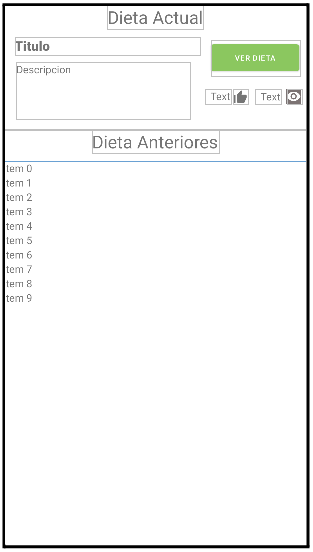
\includegraphics[width=0.4\textwidth]{Images/Capitulo7/dietaview.png}
        \caption{Elementos de la vista Dieta Actual}
    \label{fig:dietaview}
\end{figure}

\begin{figure}[H]
    \centering
    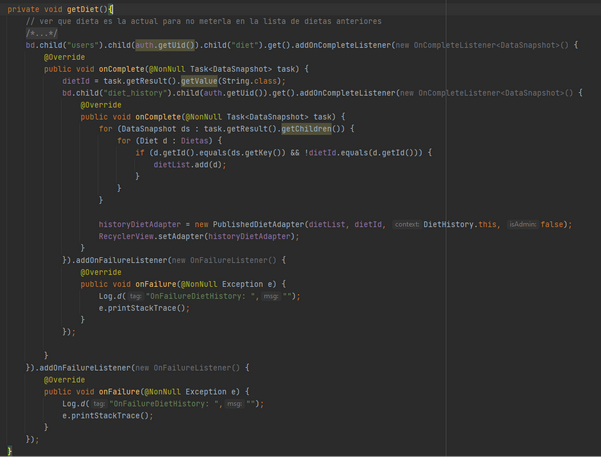
\includegraphics[width=\textwidth]{Images/Capitulo7/getdiet.png}
        \caption{Código de la función \texttt{getDiet()}}
    \label{fig:getdiet}
\end{figure}

\begin{figure}[H]
    \centering
    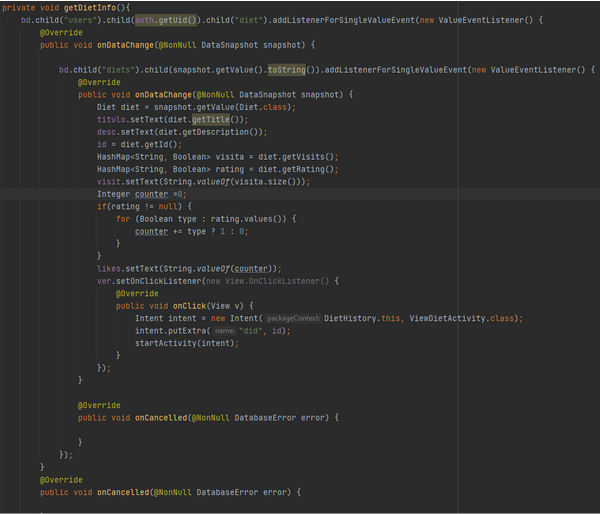
\includegraphics[width=\textwidth]{Images/Capitulo7/getdietinfo.png}
        \caption{Código de la función \texttt{getDietInfo()}}
    \label{fig:getdietinfo}
\end{figure}

\subsection{Iniciar sesión}
La primera pantalla de la aplicación corresponde al módulo de login (ver figura \ref{fig:login}), una vez cargada la pantalla contiene el logotipo de la aplicación, los campos correo electrónico y contraseña para poder iniciar sesión y los botones iniciar sesión y registrarse.

\begin{figure}[H]
    \centering
    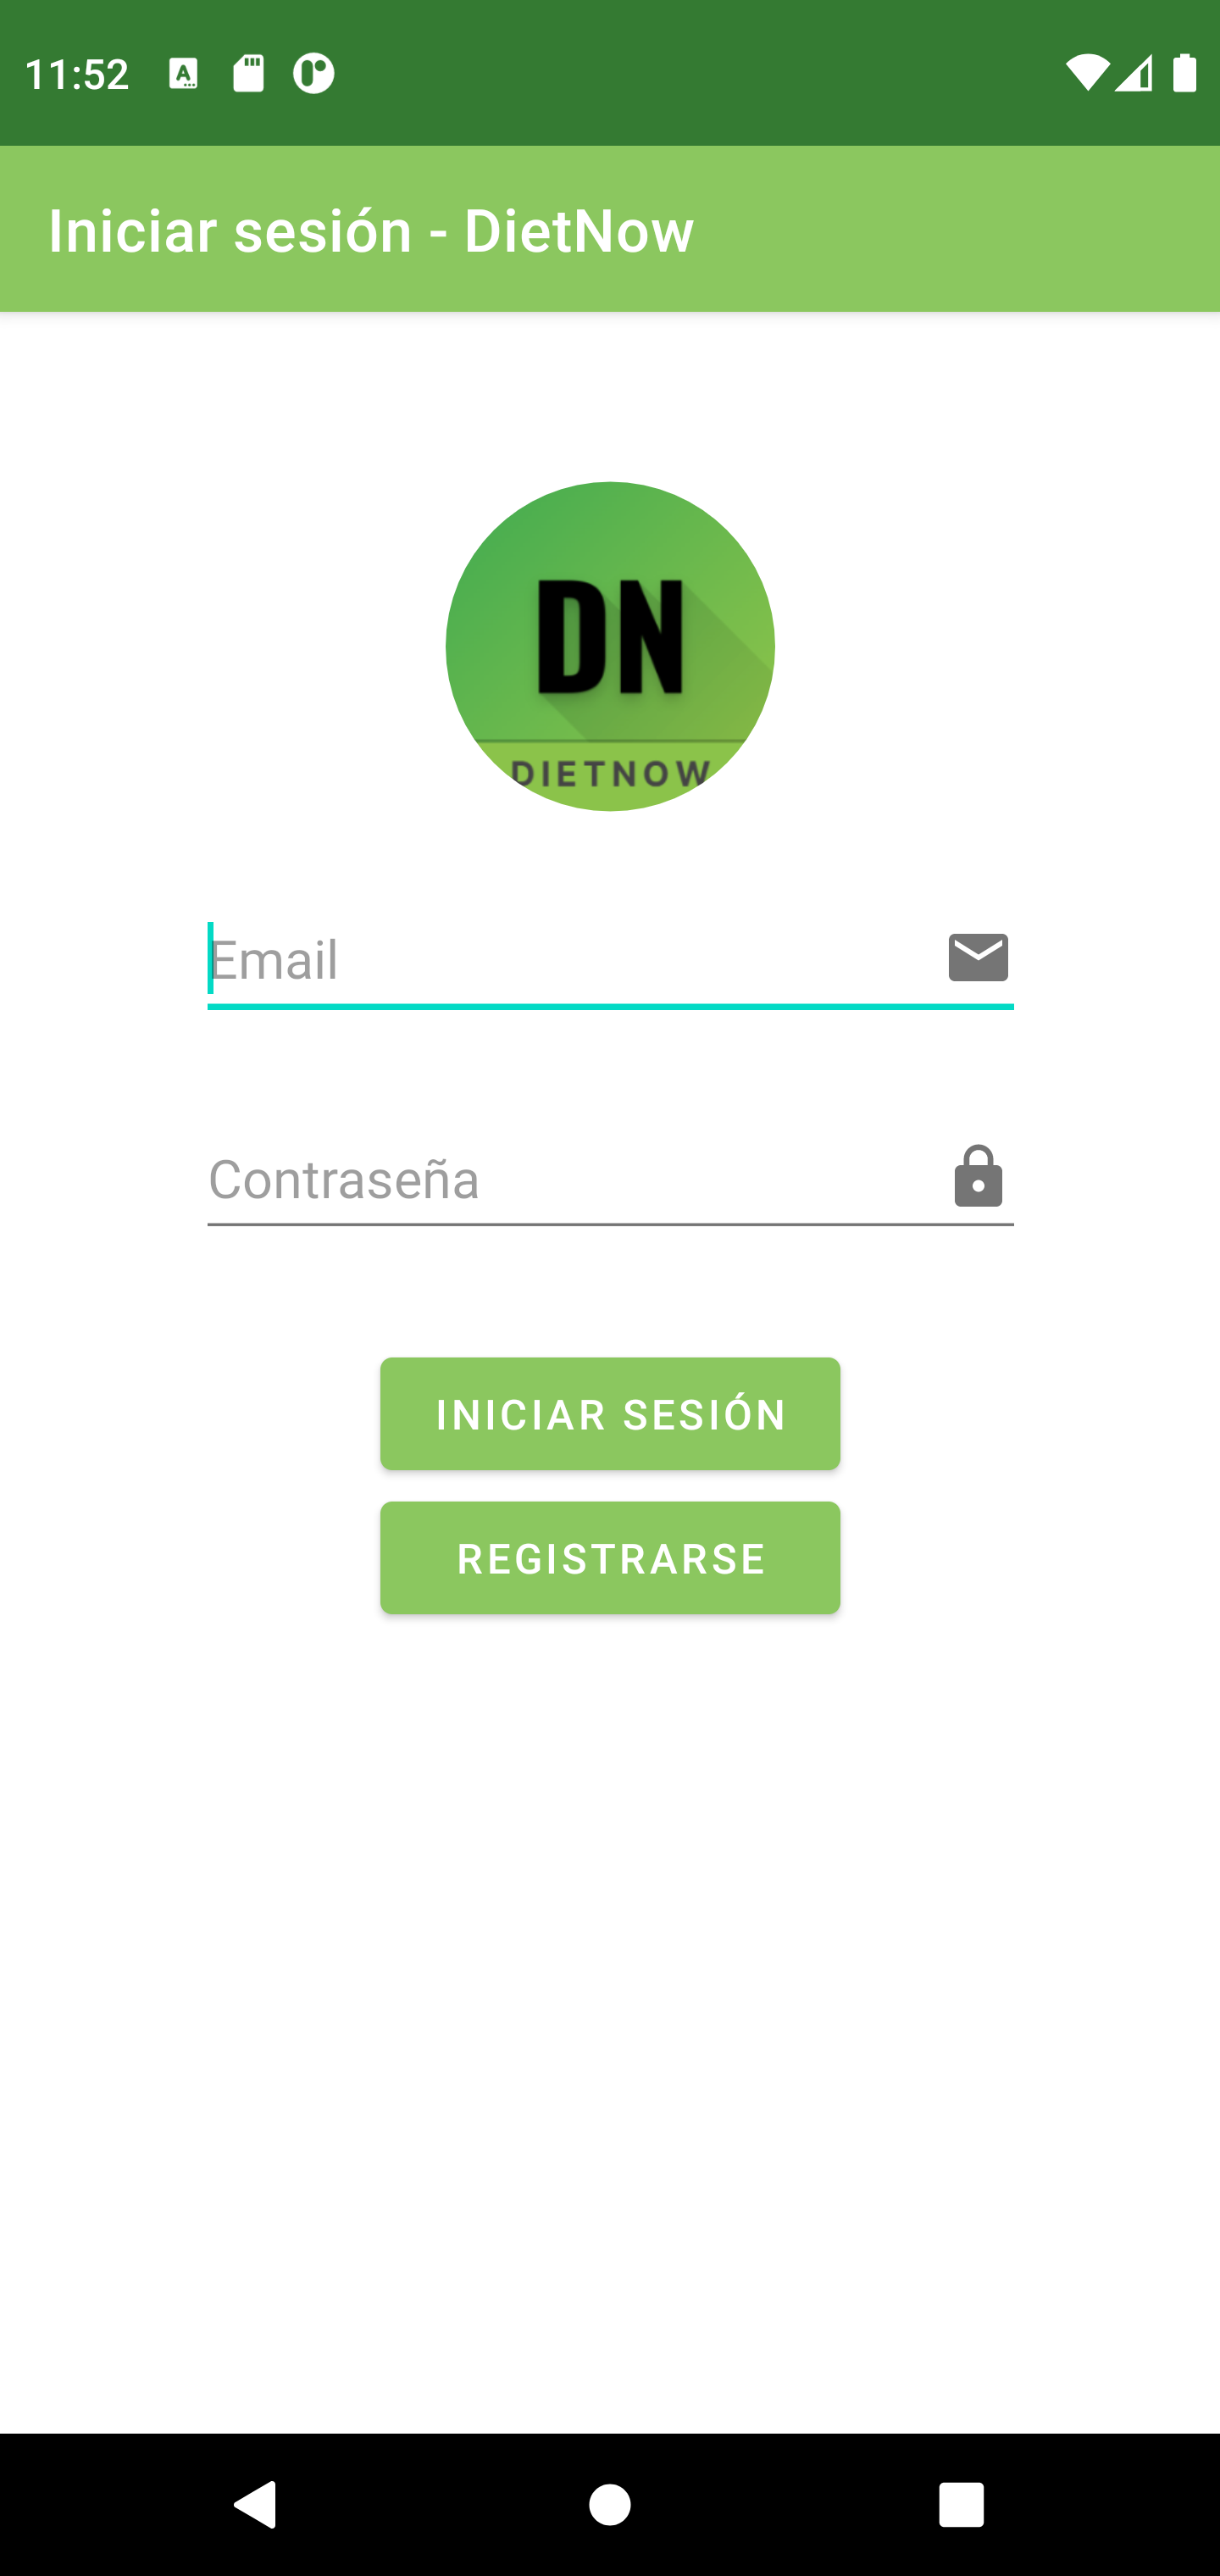
\includegraphics[width=0.5\textwidth]{Images/Capitulo7/login.png}
        \caption{Pantalla de login en la aplicación DietNow}
    \label{fig:login}
\end{figure}

En caso de que un usuario quiera darse de alta en la aplicación debe presionar ``Registrarse`` que le redirigirá a una nueva ventana donde deberá rellenar los siguientes campos:
\begin{itemize}
    \item Email
    \item Contraseña
    \item Repetir la contraseña
    \item Nombre
    \item Apellidos
    \item Edad
    \item Género
\end{itemize}
La aplicación ofrece soporte para inglés y español (ver figura \ref{fig:idiomas}). El lenguaje a utilizar se determina durante la carga de la aplicación, la cual detecta el lenguaje utilizado en el dispositivo y lo coteja con la lista de lenguajes disponibles. En caso de no encontrar coincidencias se usa el español como idioma por defecto.
\begin{figure}[H]
    \centering
    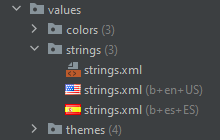
\includegraphics[width=0.3\textwidth]{Images/Capitulo7/idiomas.png}
    \caption{Lista de idiomas soportados por la aplicación DietNow}
    \label{fig:idiomas}
\end{figure}

Se pueden incluir otros idiomas de manera sencilla, añadiendo un nuevo fichero con las traducciones en el nuevo idioma. En la figura \ref{fig:idiomastext} se puede ver un ejemplo de un archivo de traducciones.
\begin{figure}[H]
    \centering
    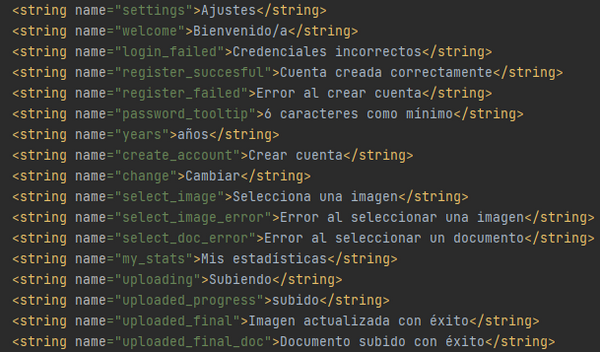
\includegraphics[width=\textwidth]{Images/Capitulo7/idiomastext.png}
    \caption{Fragmento del código del fichero con texto traducido}
    \label{fig:idiomastext}
\end{figure}

\subsubsection{Registrarse en la aplicación}
En caso de que el usuario que se encuentre en el login no tenga cuenta pulsando el botón ``Registrarse`` accederá a la vista de la figura \ref{fig:register} donde debe introducir los campos requeridos para poder registrarse en la aplicación.
\begin{figure}[H]
    \centering
    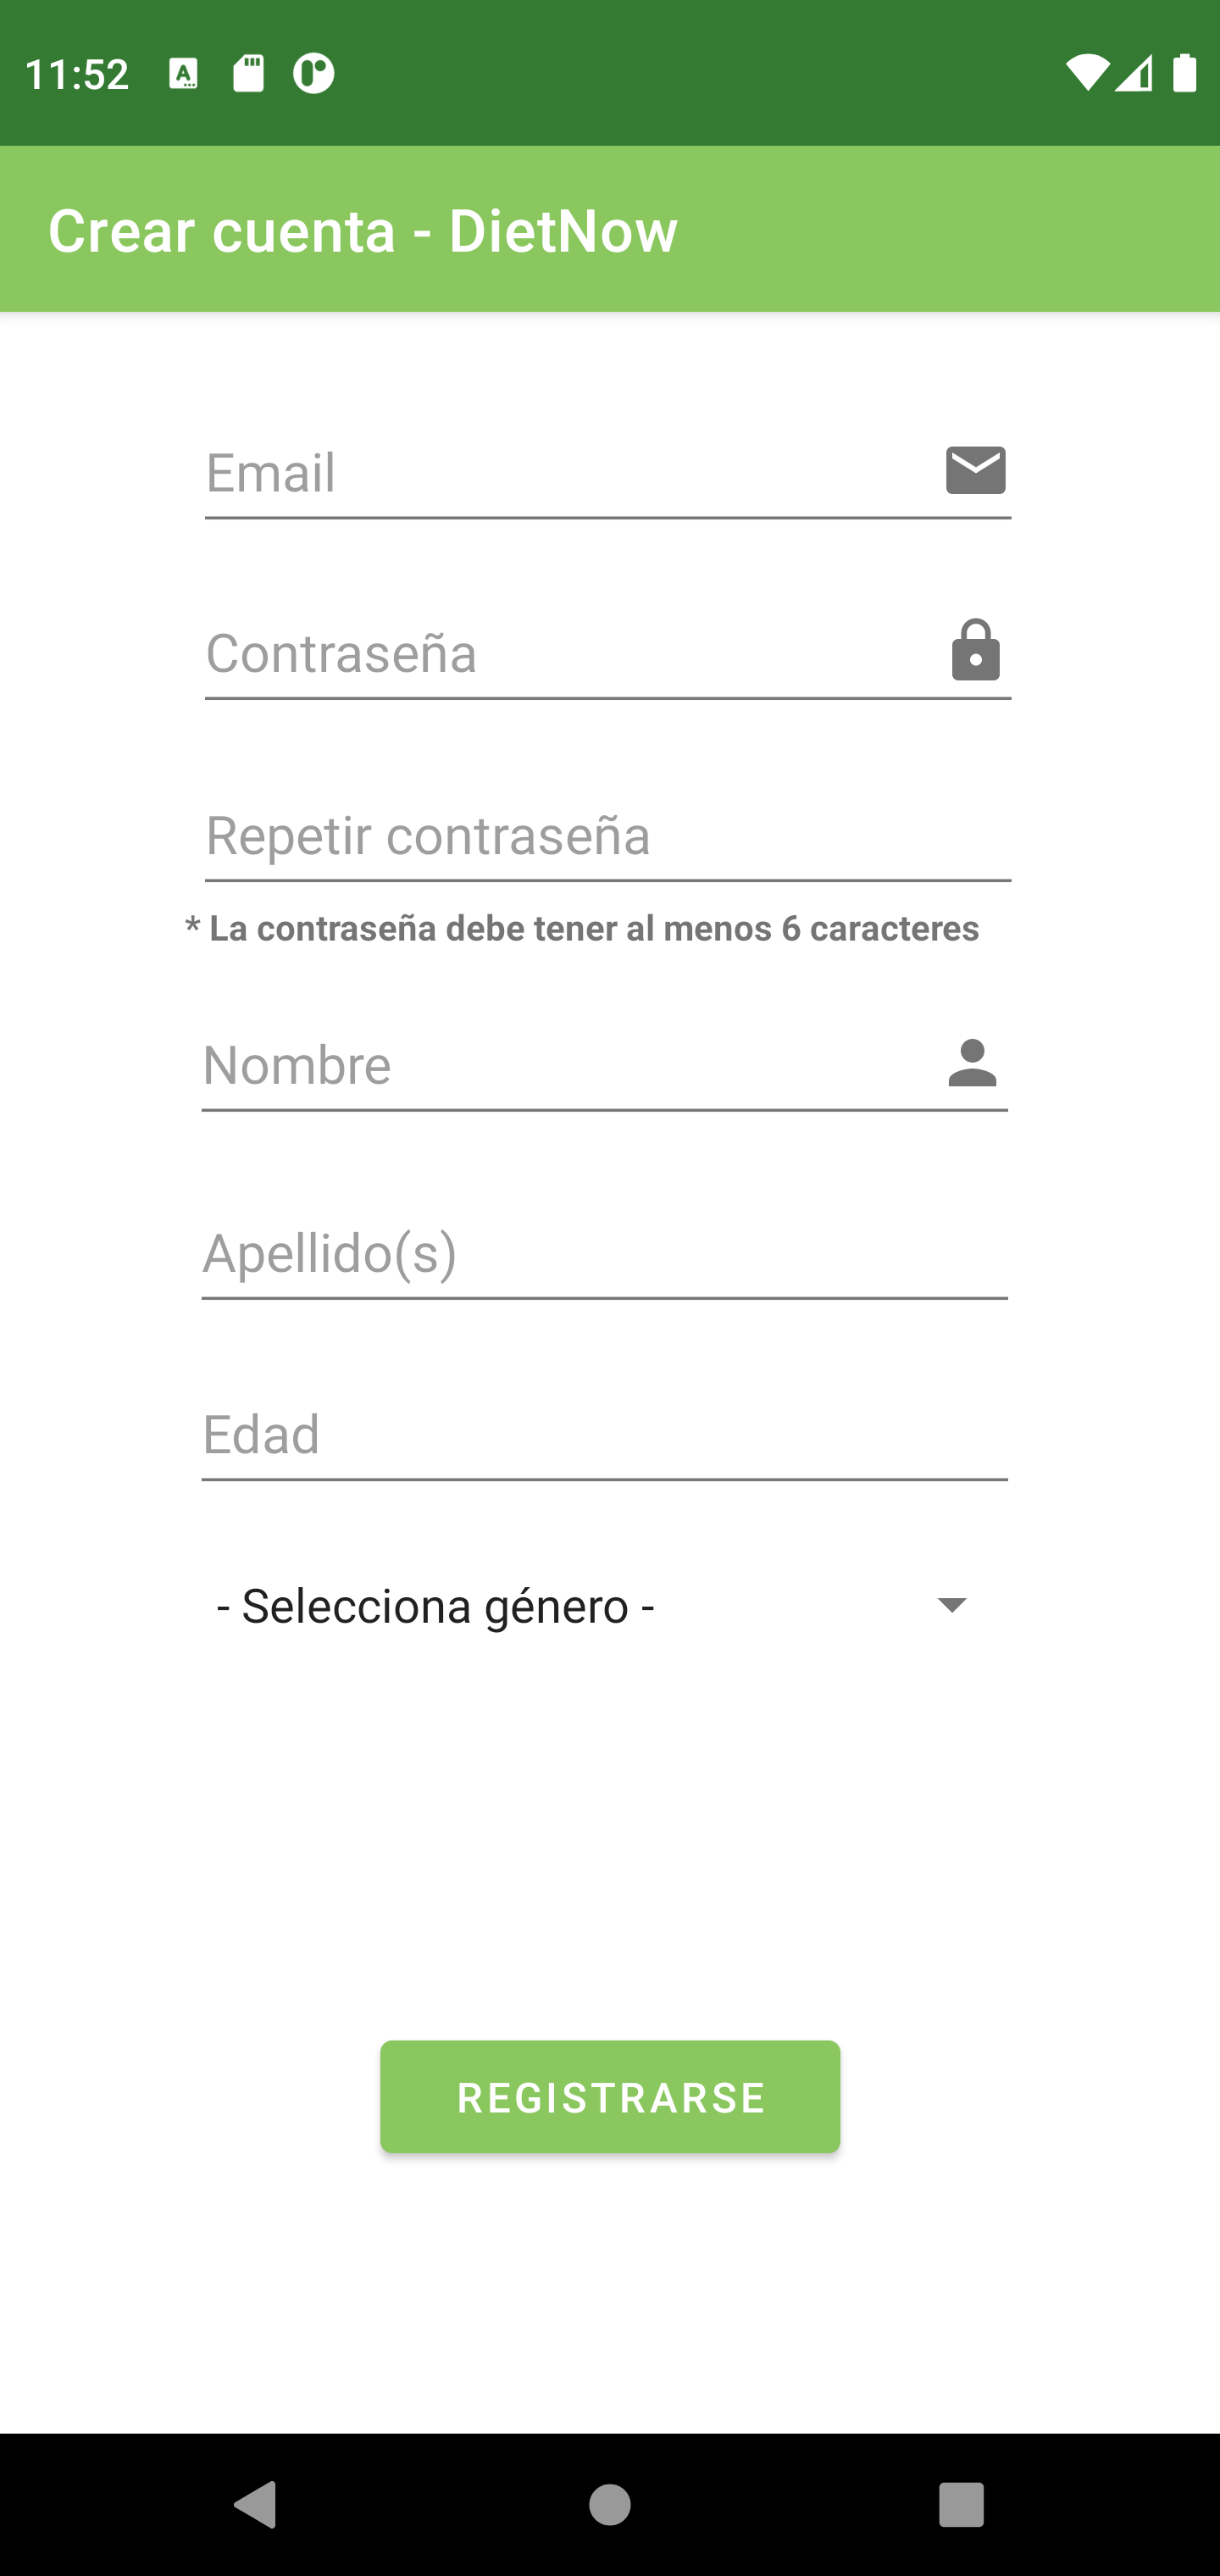
\includegraphics[width=0.5\textwidth]{Images/Capitulo7/register.png}
        \caption{Formulario de registro en la aplicación DietNow}
    \label{fig:register}
\end{figure}
Una vez introducidos los campos requeridos y tras pulsar en el botón de registrarse, se inicia sesión con la cuenta creada.

Para realizar la funcionalidad descrita anteriormente se ha creado la actividad de las figuras \ref{fig:codereg1} y \ref{fig:codereg2}:
\begin{figure}[H]
    \centering
    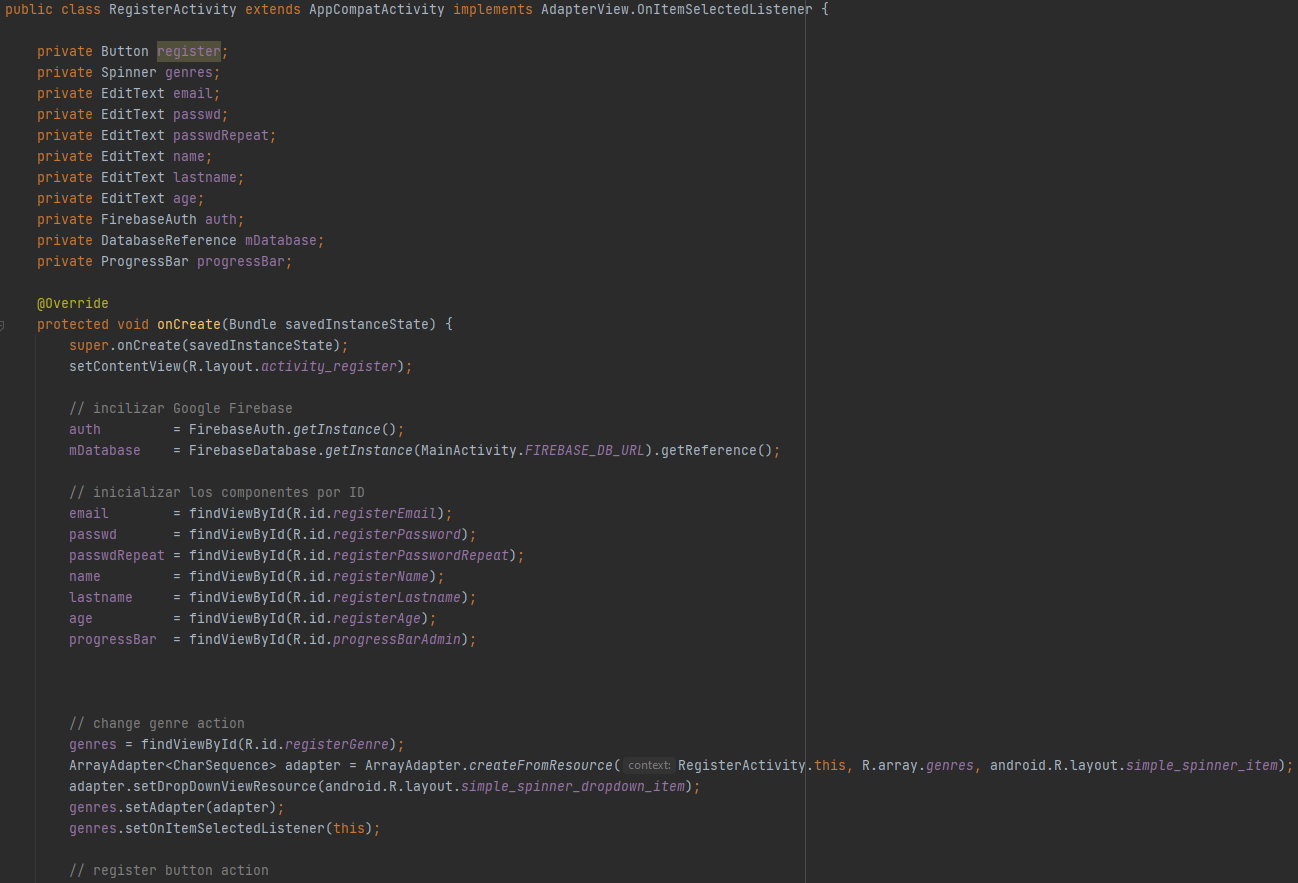
\includegraphics[width=\textwidth]{Images/Capitulo7/codereg1.png}
        \caption{Fragmento de código de la creación de la actividad \texttt{Register}}
    \label{fig:codereg1}
\end{figure}
\begin{figure}[H]
    \centering
    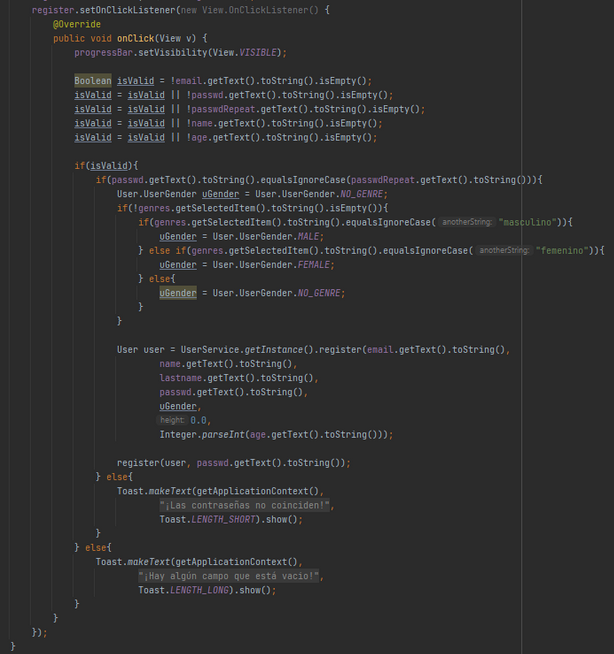
\includegraphics[width=\textwidth]{Images/Capitulo7/codereg2.png}
        \caption{Fragmento de código del botón registrar del formulario}
    \label{fig:codereg2}
\end{figure}
En la actividad indicada anteriormente, se hace referencia mediante \texttt{setContentView (R.layout.activityRegister)} a la vista indicada en la figura \ref{fig:register} y se inicializan las referencias a Realtime Database y a Authentication. En esta última referencia, se guarda la información para el inicio de sesión de los usuarios de la aplicación. Dicha referencia guarda el usuario que se encuentra \textit{logueado} en la aplicación después de haber iniciado sesión.
Al igual que en el resto de vistas se inicializan los componentes de la vista, en este caso los botones y los campos de edición de texto.
Para el selector de género (ver figura \ref{fig:selector}) se ha utilizado un adaptador que permite seleccionar un elemento dentro de una lista.
\begin{figure}[H]
    \centering
    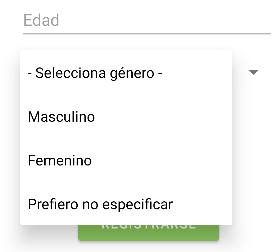
\includegraphics[width=0.3\textwidth]{Images/Capitulo7/selector.png}
    \caption{Selector de género en el formulario de registro}
    \label{fig:selector}
\end{figure}
Posteriormente se establece la acción relativa al botón de registrarse. El usuario debe de haber introducido los campos requeridos correctamente, así como haber introducido la misma contraseña con el tamaño especificado en las dos ocasiones.

Después de haber comprobado que se han introducido los datos con el formato solicitado, se crea un usuario llamando al método \texttt{register()} de la clase \texttt{UserService} (ver figura \ref{fig:userservice}).

\begin{figure}[H]
    \centering
    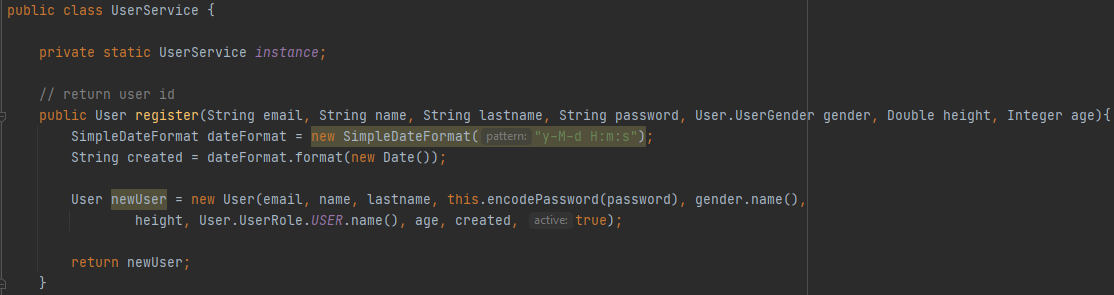
\includegraphics[width=\textwidth]{Images/Capitulo7/userservice.png}
    \caption{Código de la función \texttt{register()} de \texttt{UserService}}
    \label{fig:userservice}
\end{figure}
Tras haber creado la instancia del usuario se registrará al usuario en la base de datos (ver figura \ref{fig:registerfunct}).

\begin{figure}[H]
    \centering
    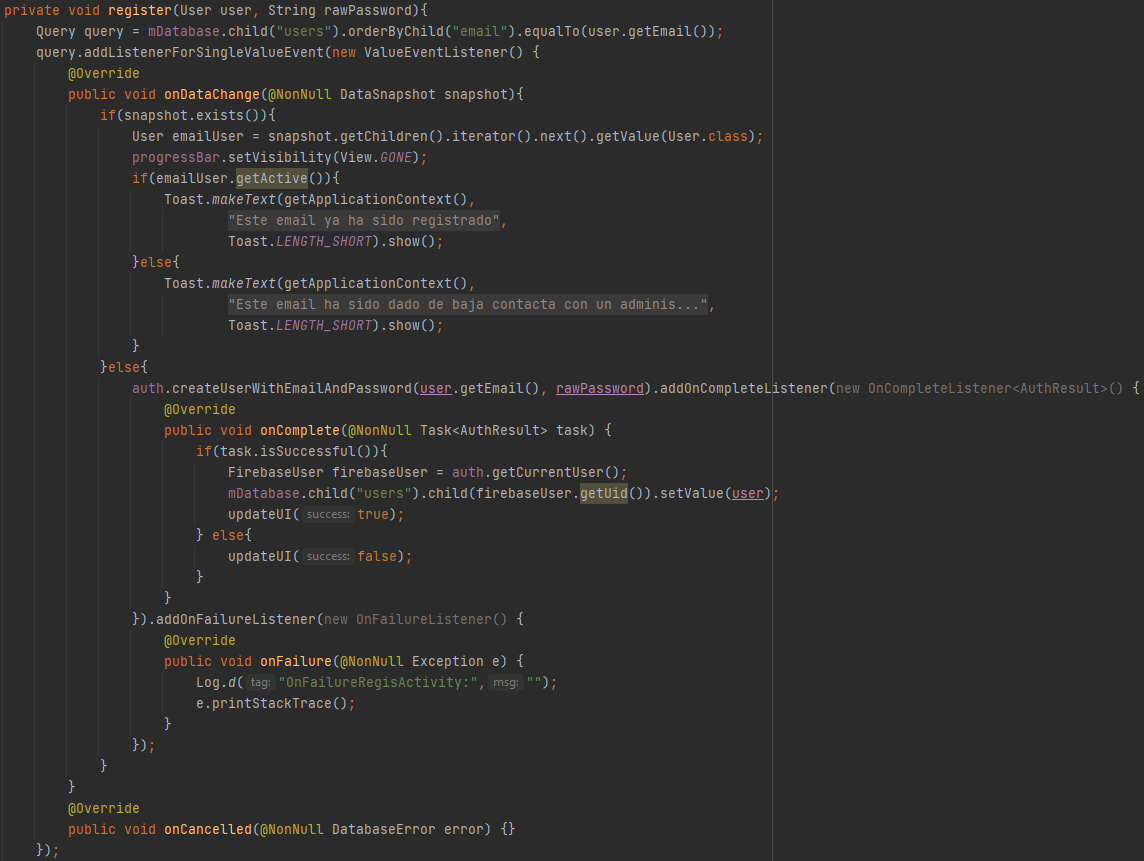
\includegraphics[width=\textwidth]{Images/Capitulo7/registerfunct.png}
        \caption{Código de la función \texttt{register()} del formulario}
    \label{fig:registerfunct}
\end{figure}
En dicho método, se accede a la tabla de la base datos de usuario, ordenando los resultados por email para posteriormente comprobar si existe un usuario activo con el email indicado, un administrador ha dado de baja al usuario o no existe ese usuario en la base de datos. Si el usuario no existe en la base de datos se registra al usuario en el módulo de autenticación mediante el método \texttt{createUserWithEmailAndPassword()}.

Si se ha registrado correctamente en el módulo de Autenticación, se crea una entrada de ese usuario en Realtime Database en la tabla de usuarios:

\texttt{mDatabase.child(users).child(firebaseUser.getUid()).setValue(user);}
(ver figura \ref{fig:bdreg}).

\begin{figure}[H]
    \centering
    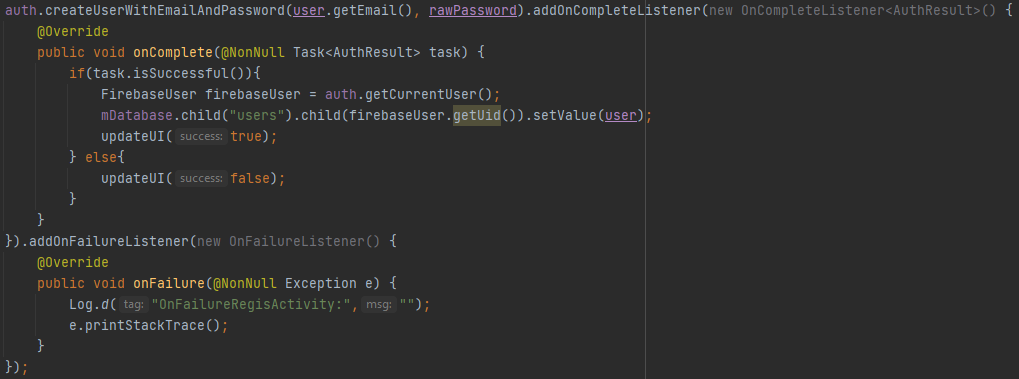
\includegraphics[width=\textwidth]{Images/Capitulo7/bdreg.png}
        \caption{Código la consulta a la base de datos}
    \label{fig:bdreg}
\end{figure}
Después de haber creado al nuevo usuario correctamente se actualiza la vista (ver figura \ref{fig:updateui}).
\begin{figure}[H]
    \centering
    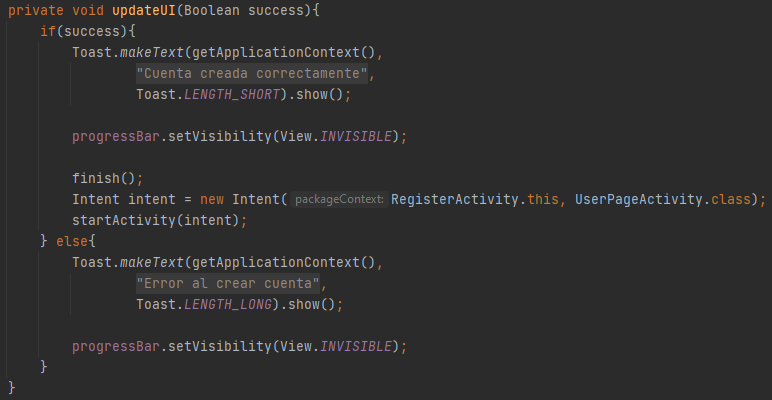
\includegraphics[width=\textwidth]{Images/Capitulo7/updateui.png}
        \caption{Código de la función que actualiza la vista}
    \label{fig:updateui}
\end{figure}

En el método \texttt{updateUI()}, se muestra un mensaje de error en el caso de no haber registrado correctamente al usuario y un mensaje de éxito en el caso contrario.
Se realiza un \texttt{finish()} de la actividad actual, para sacarla de la pila de llamadas y en el caso de pulsar en el botón de ir hacia atrás en el móvil, no mantenga en memoria dicha vista.\\
Posteriormente se crea un objeto \texttt{Intent}, el cual se utiliza para realizar redirecciones entre vistas. En este caso y, después de haber \textit{iniciado sesión} correctamente al usuario, se redirige a la actividad de \texttt{UserPageActivity()} (ver figura \ref{fig:userpageact}) la cual en su método \texttt{OnCreate()} hace referencia a la vista de la figura \ref{fig:udashboard} que se cargará.

\begin{figure}[H]
    \centering
    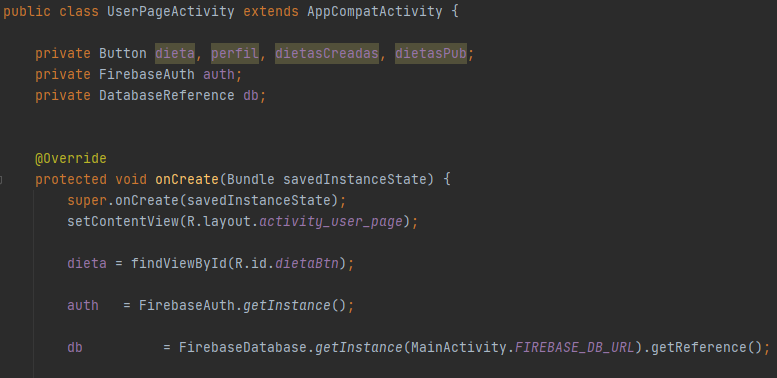
\includegraphics[width=\textwidth]{Images/Capitulo7/userpageact.png}
    \caption{Código de \texttt{UserPageActivity()}}
    \label{fig:userpageact}
\end{figure}

\begin{figure}[H]
    \centering
    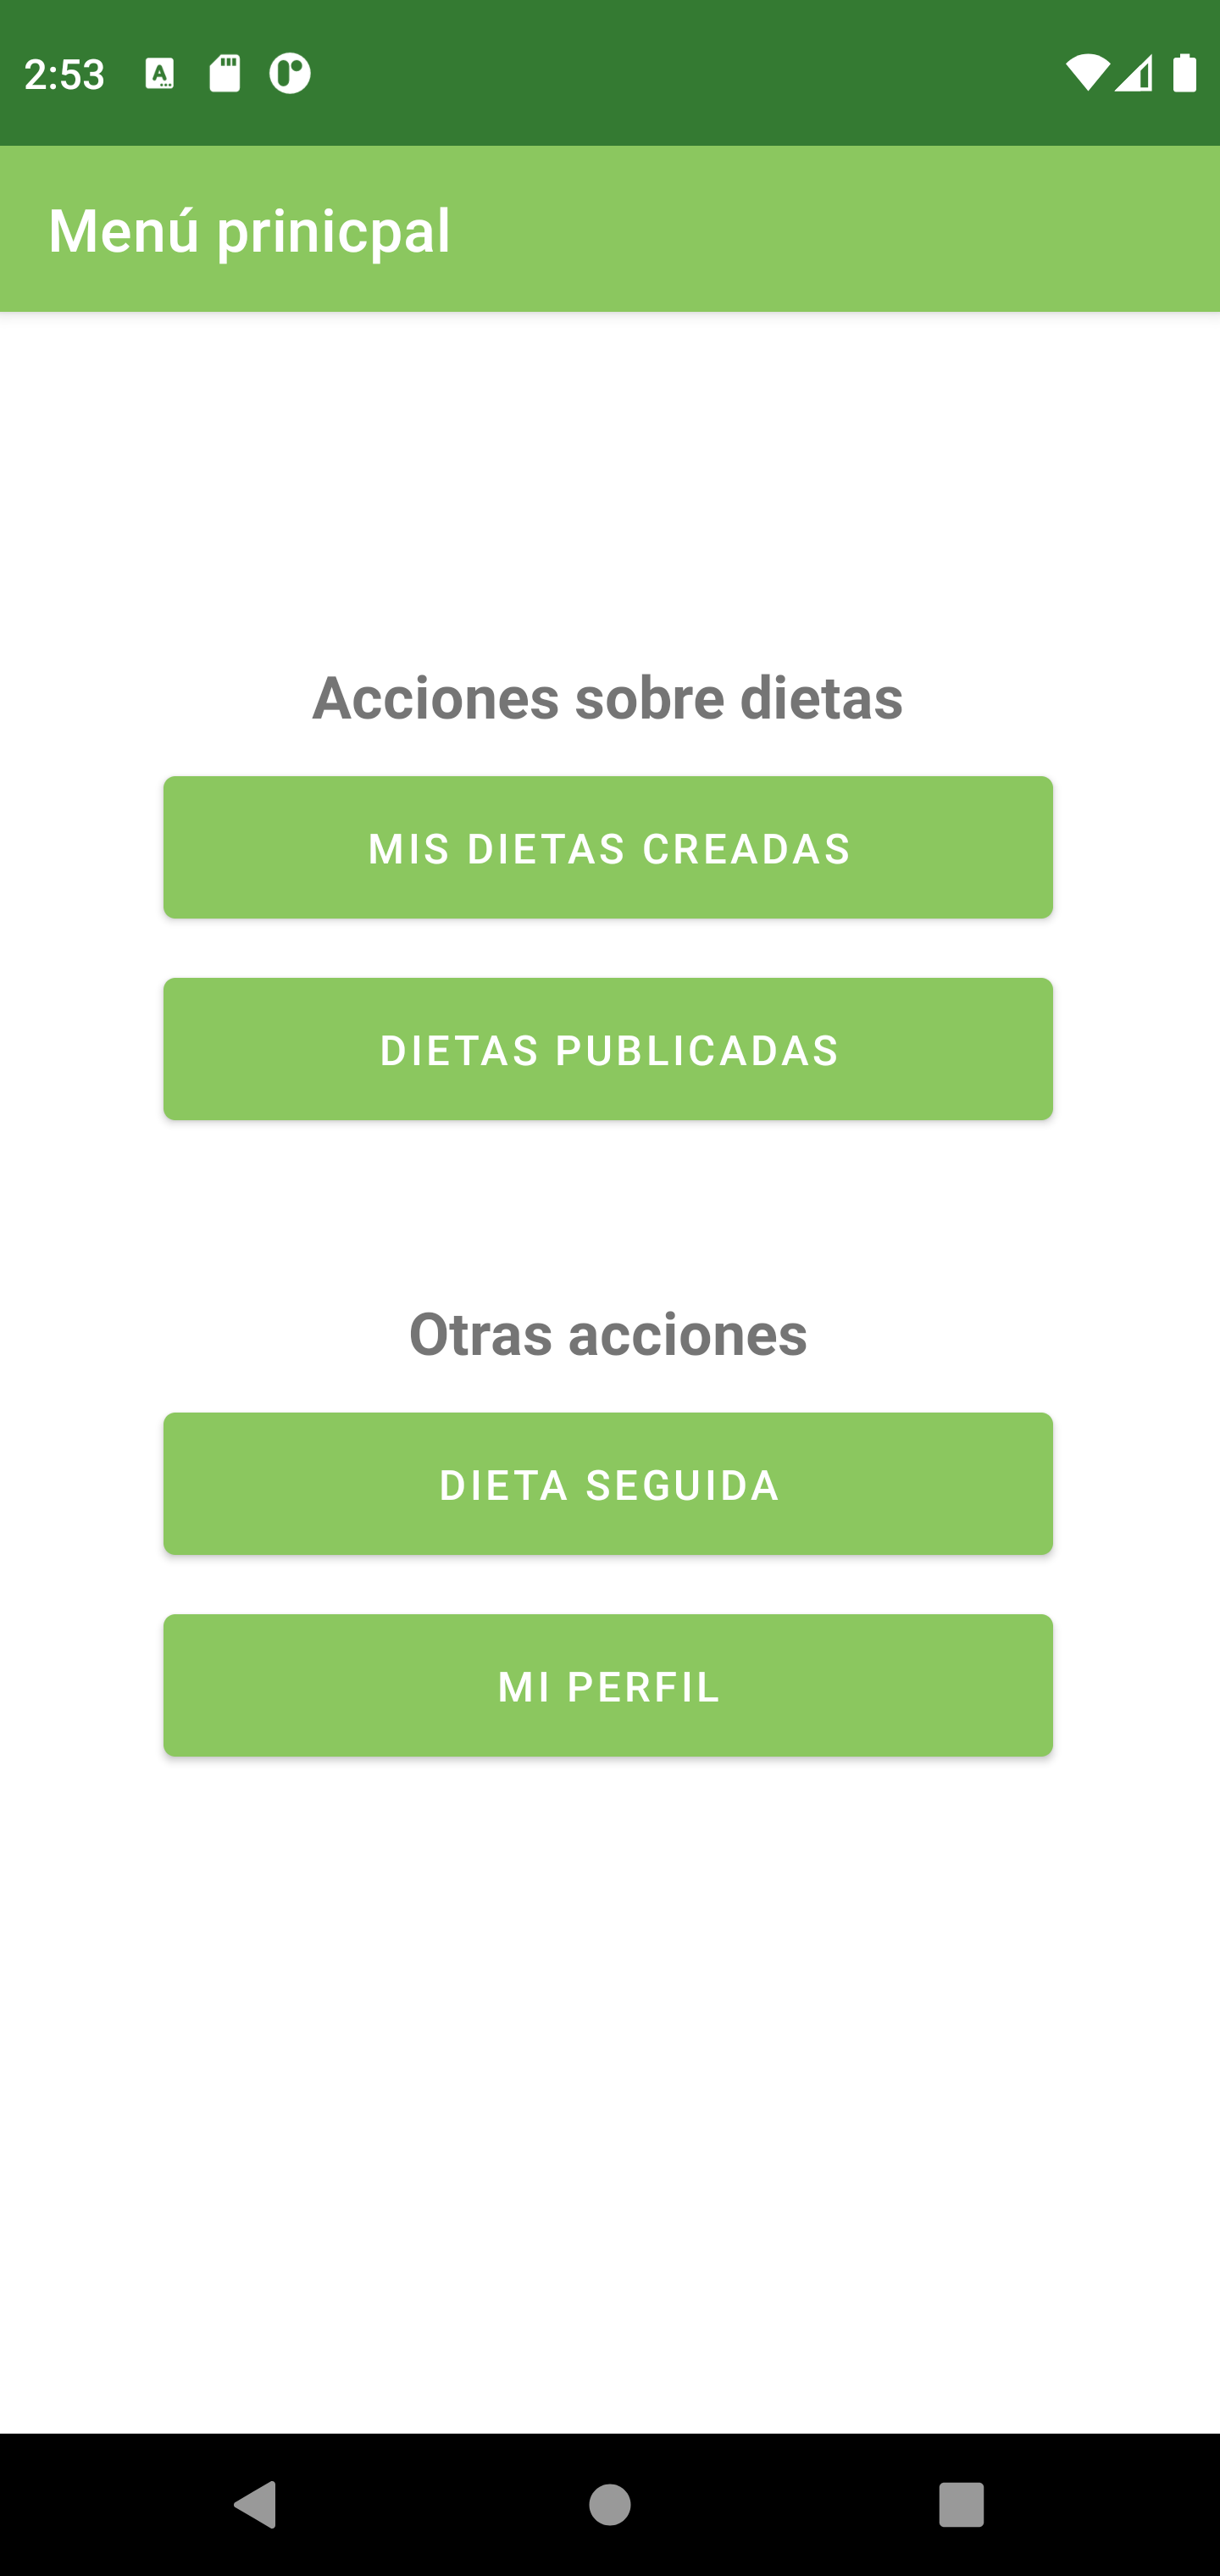
\includegraphics[width=0.5\textwidth]{Images/Capitulo7/udashboard.png}
    \caption{Vista del menú principal de un usuario}
    \label{fig:udashboard}
\end{figure}

\subsection{Crear dieta y modificarla}
Esta vista sirve para crear una dieta, añadiendo su título y su descripción. Posteriormente en la vista de modificar dieta se pueden editar los campos anteriormente mencionados así como añadir alimentos de forma manual o con la cámara y subir documentos relativos a la dieta.

Para realizar esta funcionalidad desde la actividad \texttt{UserPageActivity}, en el menú principal, mostrado en la figura \ref{fig:udashboard}, se realiza un \texttt{Intent} cuando se pulsa sobre del botón de ``Mis dietas creadas`` a la actividad \texttt{MyDietsActivity} (ver figura \ref{fig:dietascreadas}).

\begin{figure}[H]
    \centering
    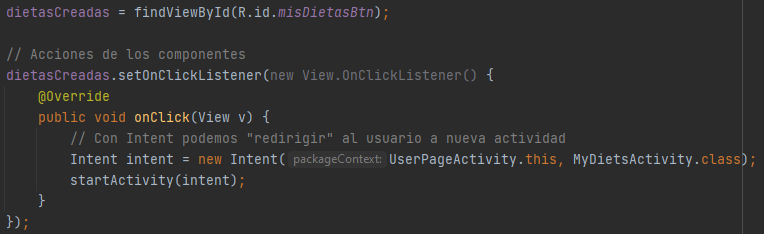
\includegraphics[width=\textwidth]{Images/Capitulo7/dietascreadas.png}
        \caption{Código del evento asociado al botón ``Mis dietas creadas``}
    \label{fig:dietascreadas}
\end{figure}

Después de haber pulsado el botón desde el método \texttt{OnCreate()} de \texttt{MyDietsActivity} (ver figura \ref{fig:dietascreadas}) se hace referencia a la vista que se muestra en la figura \ref{fig:misdietas} para asociar dicha vista con la actividad.

\begin{figure}[H]
    \centering
    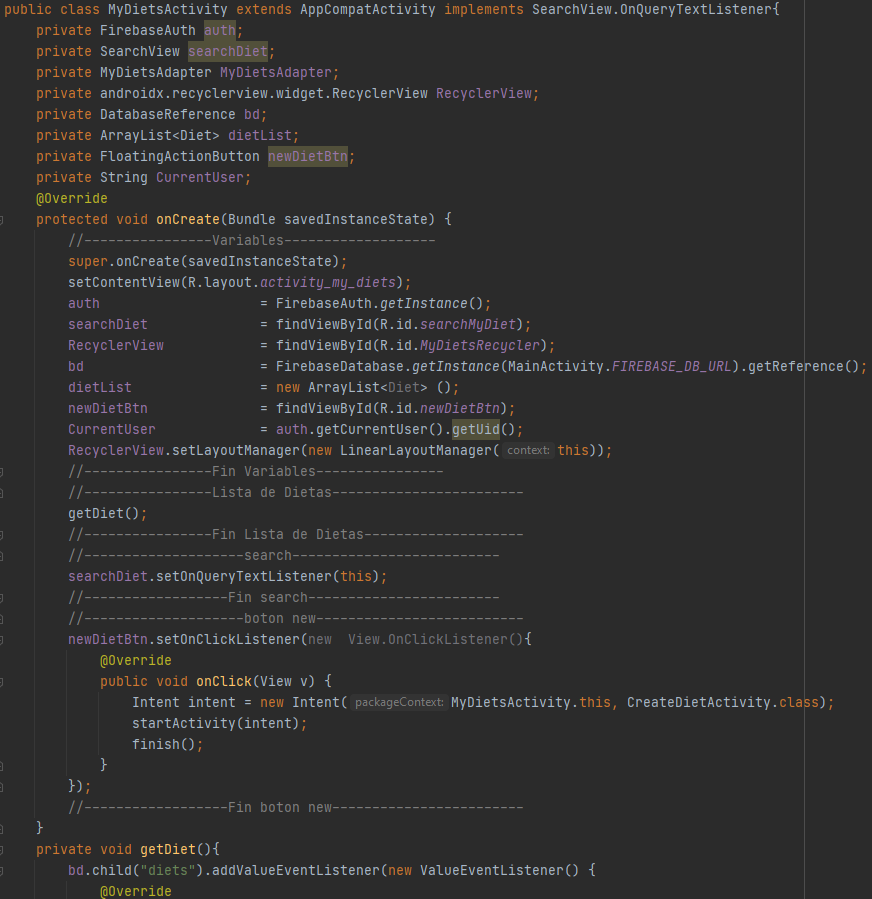
\includegraphics[width=0.6\textwidth]{Images/Capitulo7/mydietsact.png}
        \caption{Código de la actividad \texttt{MyDietsActivity}}
    \label{fig:mydietsact}
\end{figure}

\begin{figure}[H]
    \centering
    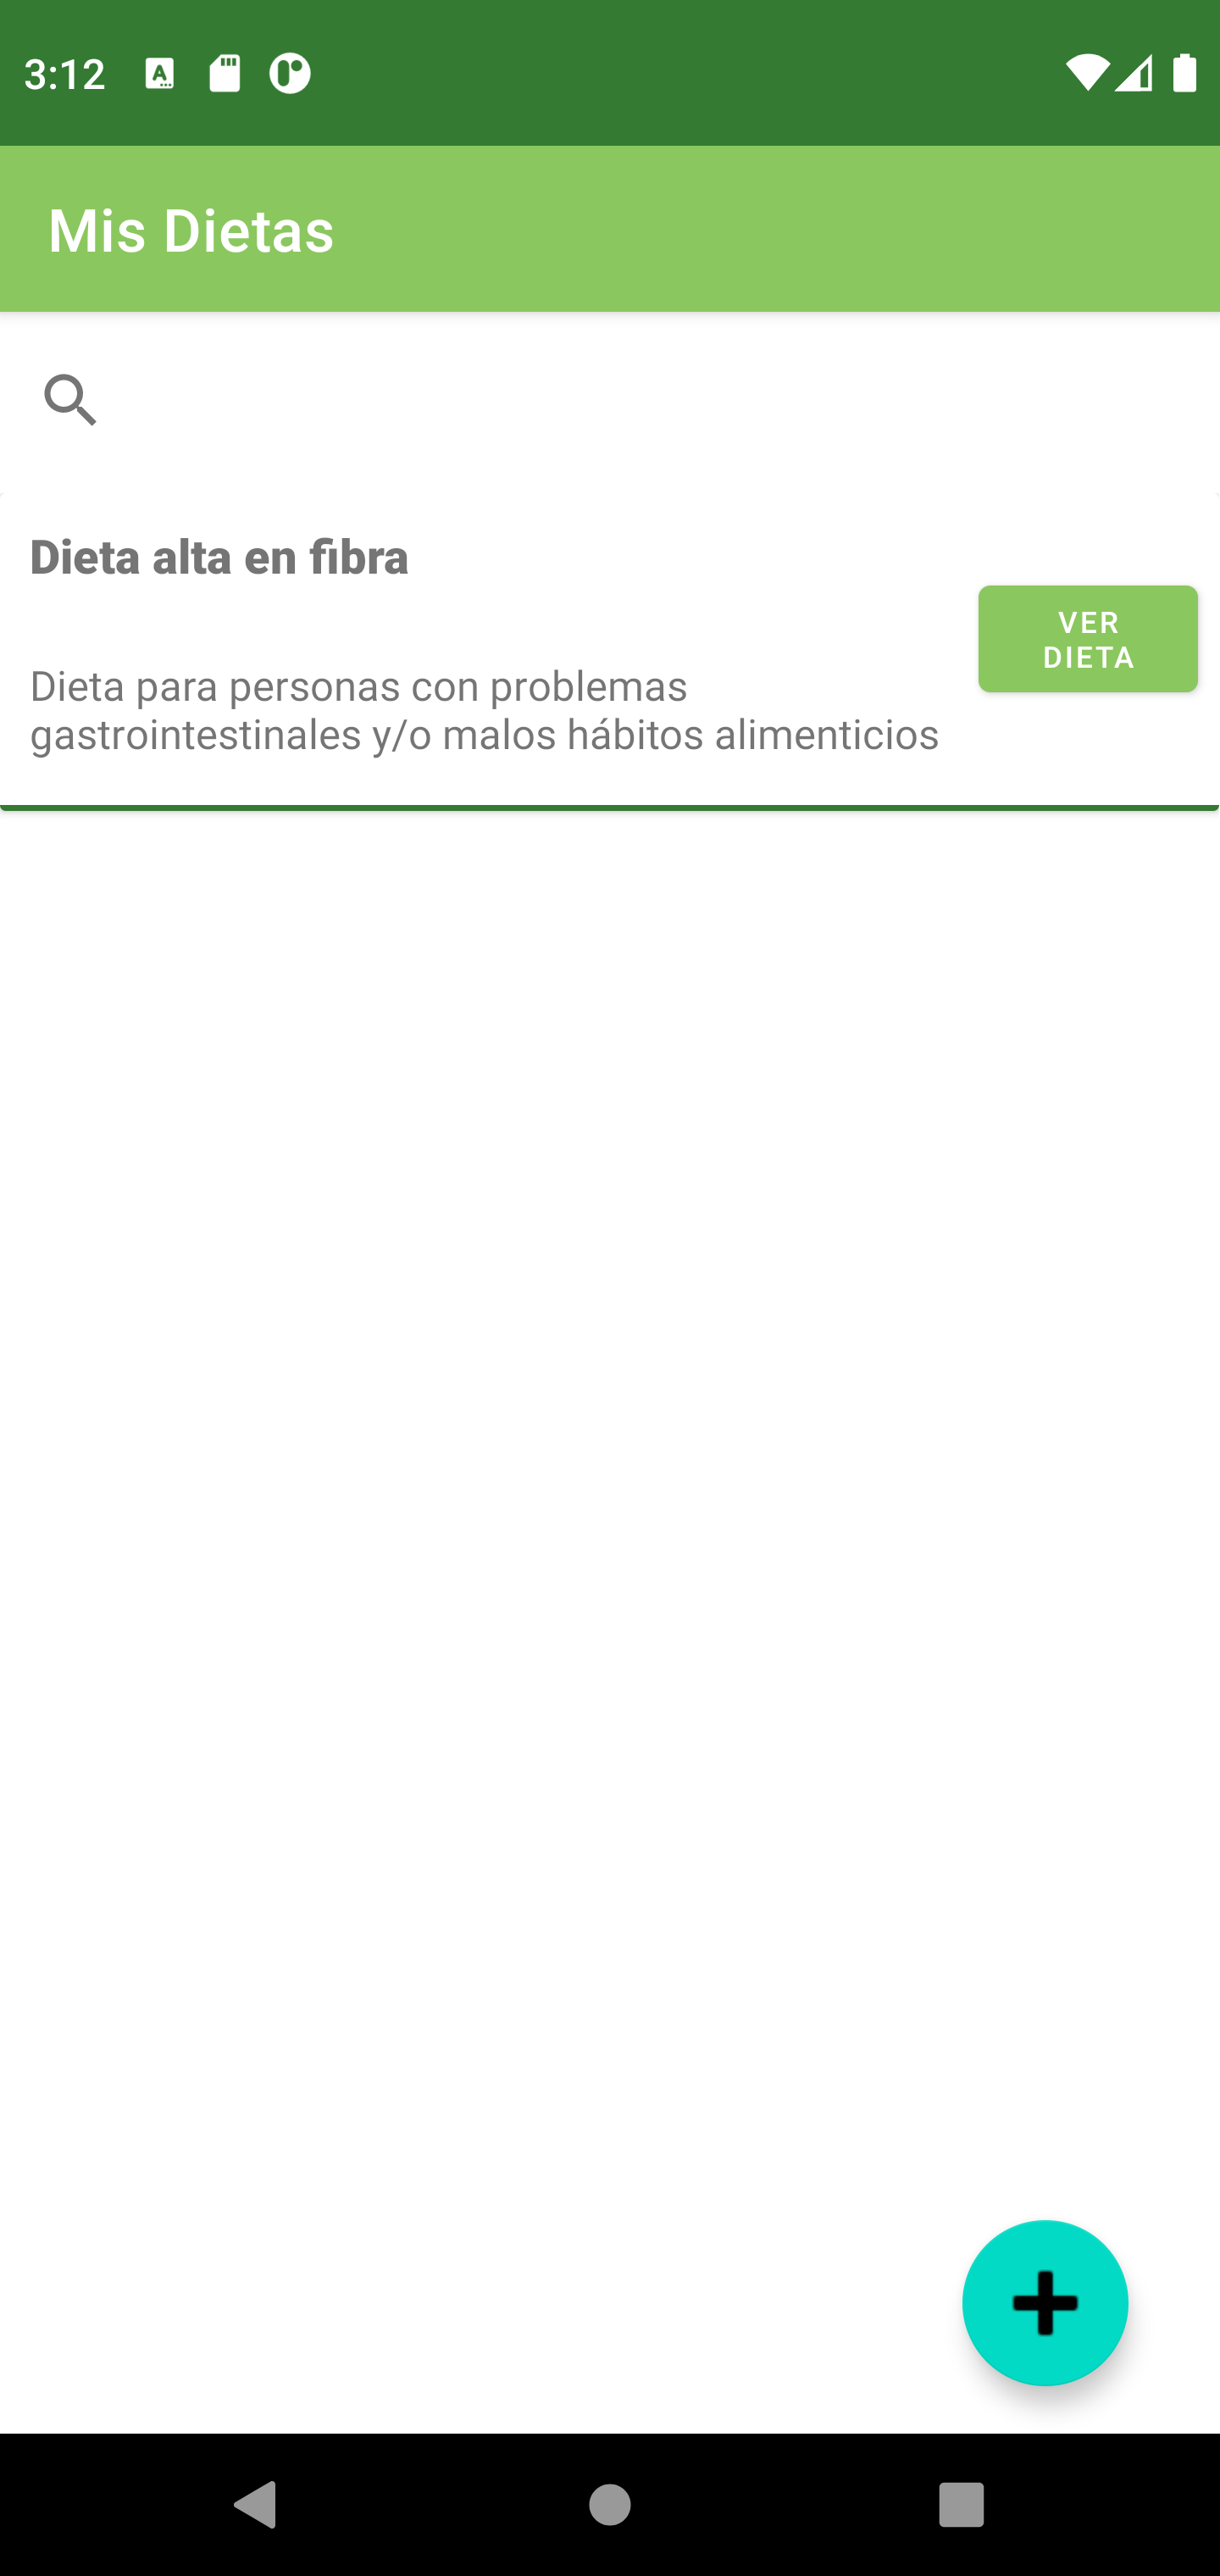
\includegraphics[width=0.5\textwidth]{Images/Capitulo7/misdietas.png}
        \caption{Vista “Mis dietas”}
    \label{fig:misdietas}
\end{figure}

En dicha vista se cargan todas las dietas que ha creado el usuario, para ello se crea un \texttt{Adapter} para poder ir mostrando dinámicamente las distintas dietas de la aplicación.

En la figura \ref{fig:getdietcreate} se puede ver como se cargan todas las dietas que ha creado el usuario que ha iniciado sesión para posteriormente ir mostrándolas dinámicamente.

\begin{figure}[H]
    \centering
    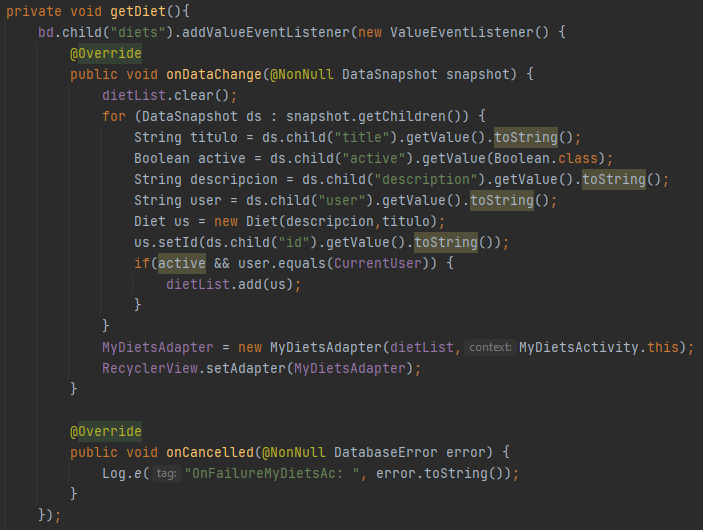
\includegraphics[width=\textwidth]{Images/Capitulo7/getdietcreate.png}
        \caption{Código de la función que carga las dietas creadas}
    \label{fig:getdietcreate}
\end{figure}

Además dentro de la vista ``Mis Dietas`` (ver figura \ref{fig:misdietas}) pulsando sobre el botón de ``+`` se añade una nueva dieta, lo cual hace que se asocie un \texttt{Intent} a la nueva actividad sobre ese botón. Posteriormente se hace un \texttt{finish()} \cite{finish_android_method} para sacar de la pila de actividades la actividad actual y cuando se pulse el botón de ir atrás en el móvil no vuelva a esa vista (ver figura \ref{fig:newdietbtn}).

\begin{figure}[H]
    \centering
    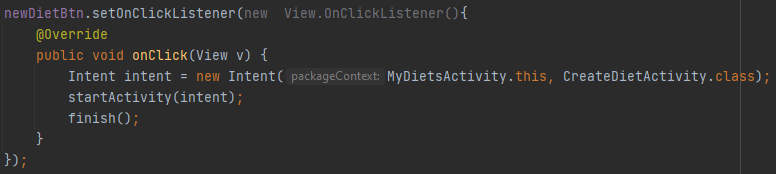
\includegraphics[width=\textwidth]{Images/Capitulo7/newdietbtn.png}
        \caption{Código de la función asociada al botón + de Mis Dietas}
    \label{fig:newdietbtn}
\end{figure}

En dicha vista (ver figura \ref{fig:creatediet}) se introduce el nombre y la descripción de la dieta y se pulsa sobre el botón de guardar para actualizar la base de datos con la nueva información (ver figura \ref{fig:createbtn}).

\begin{figure}[H]
    \centering
    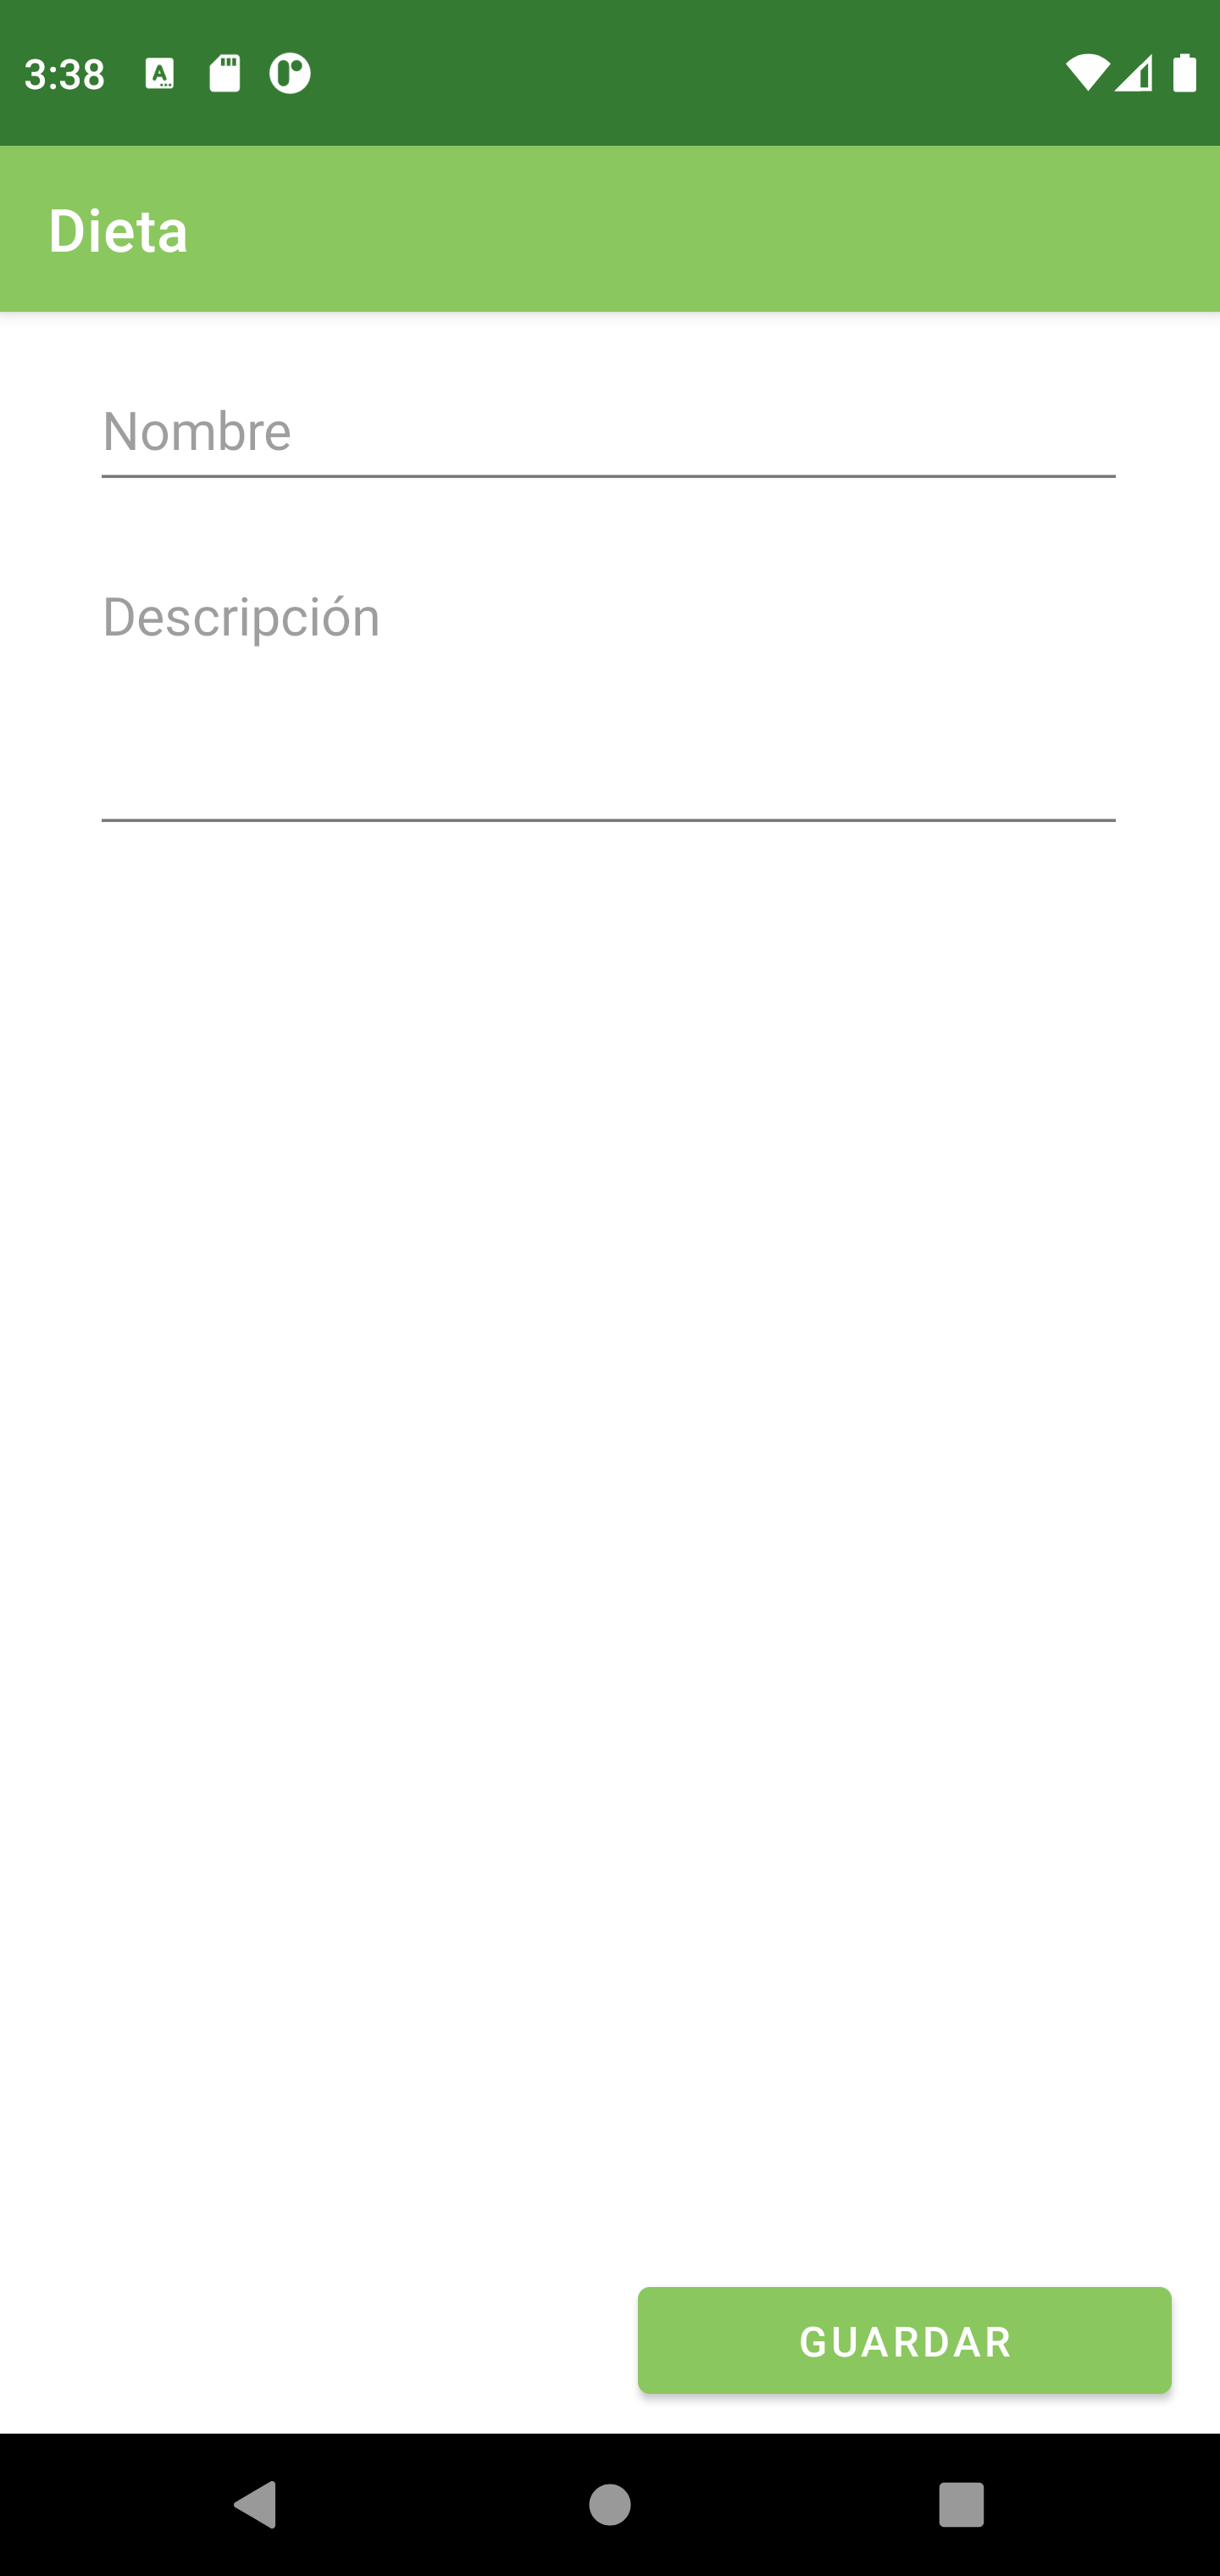
\includegraphics[width=0.5\textwidth]{Images/Capitulo7/creatediet.png}
        \caption{Vista de crear nueva dieta}
    \label{fig:creatediet}
\end{figure}

\begin{figure}[H]
    \centering
    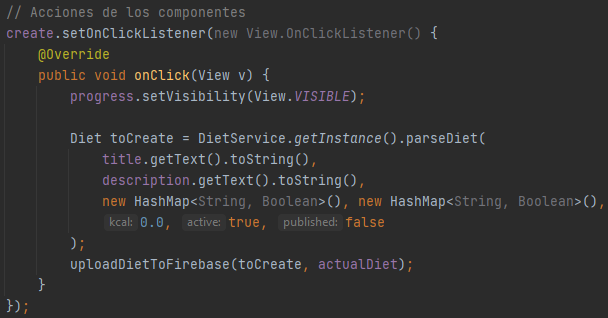
\includegraphics[width=\textwidth]{Images/Capitulo7/createbtn.png}
        \caption{Código de la función asociada al botón ``Guardar`` de crear nueva dieta}
    \label{fig:createbtn}
\end{figure}

Una vez creada la dieta en la vista de mis dietas creadas, si se pulsa sobre ver dieta se muestra la vista de ``Ver Dieta`` (ver figura \ref{fig:verdieta}). En esta vista se puede editar la dieta creada por el usuario así como publicar una dieta para que sea visible para el resto de usuarios de la aplicación. Si la dieta está despublicada solo será vista por el usuario que ha creado la dieta y ningún deportista podrá seguir la dieta.

\begin{figure}[H]
    \centering
    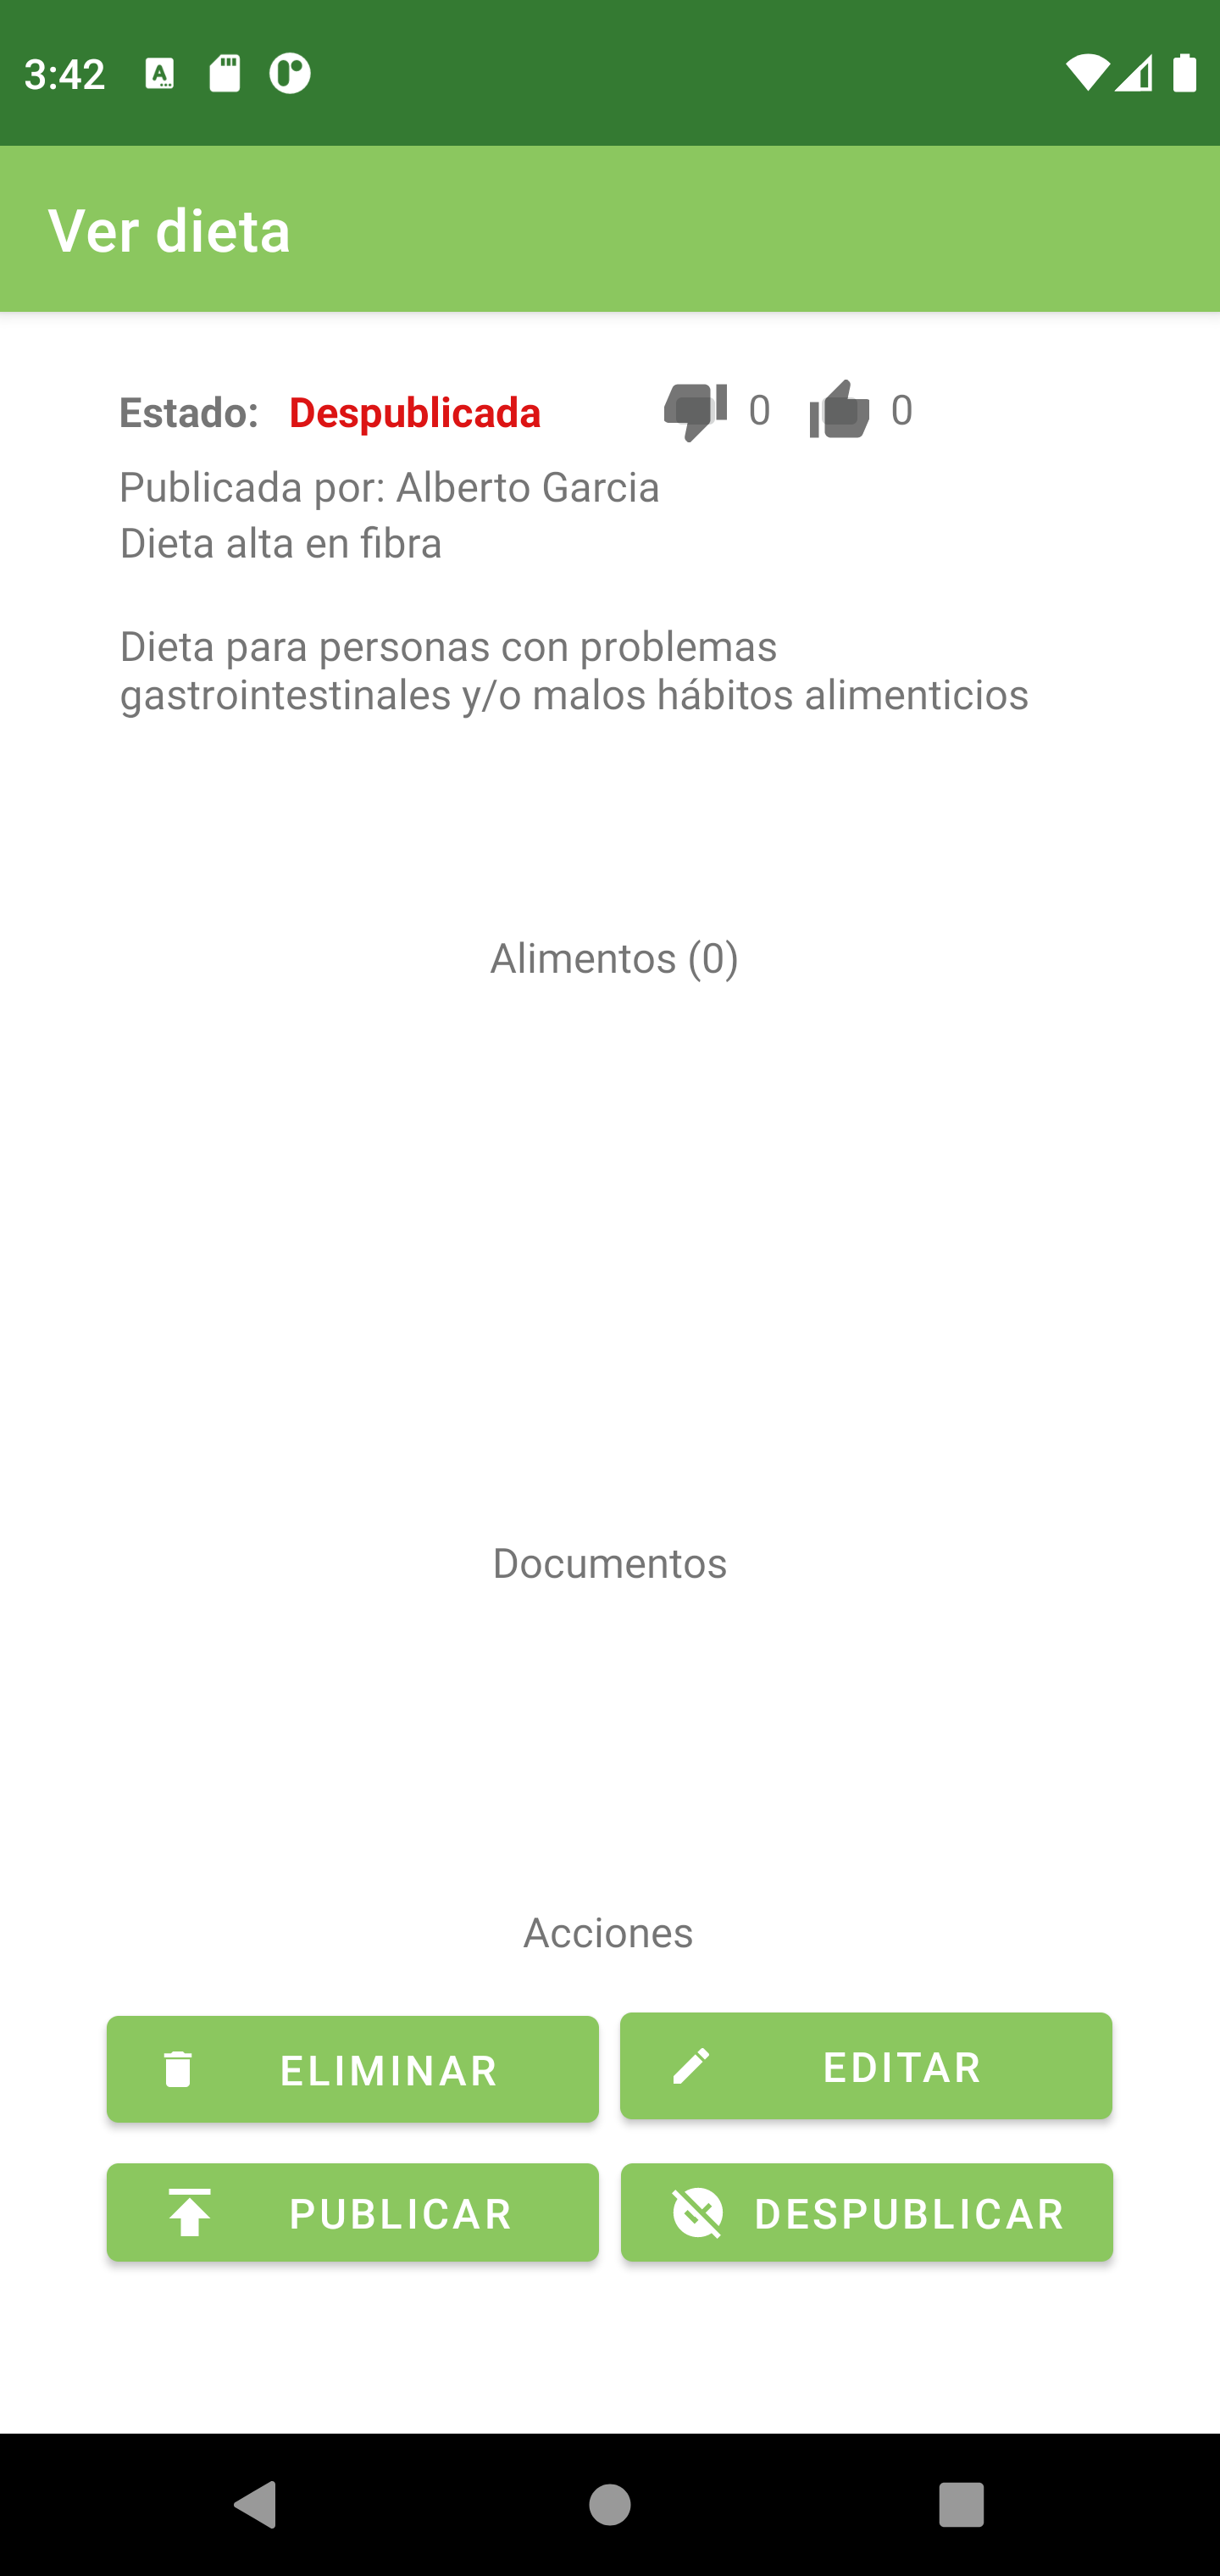
\includegraphics[width=0.5\textwidth]{Images/Capitulo7/verdieta.png}
        \caption{Vista de Ver Dieta}
    \label{fig:verdieta}
\end{figure}

Para poder introducir alimentos o subir documentos a la dieta se pulsa sobre el botón de editar donde se redirige a otra vista (ver figura \ref{fig:editardieta}). 
\begin{figure}[H]
    \centering
    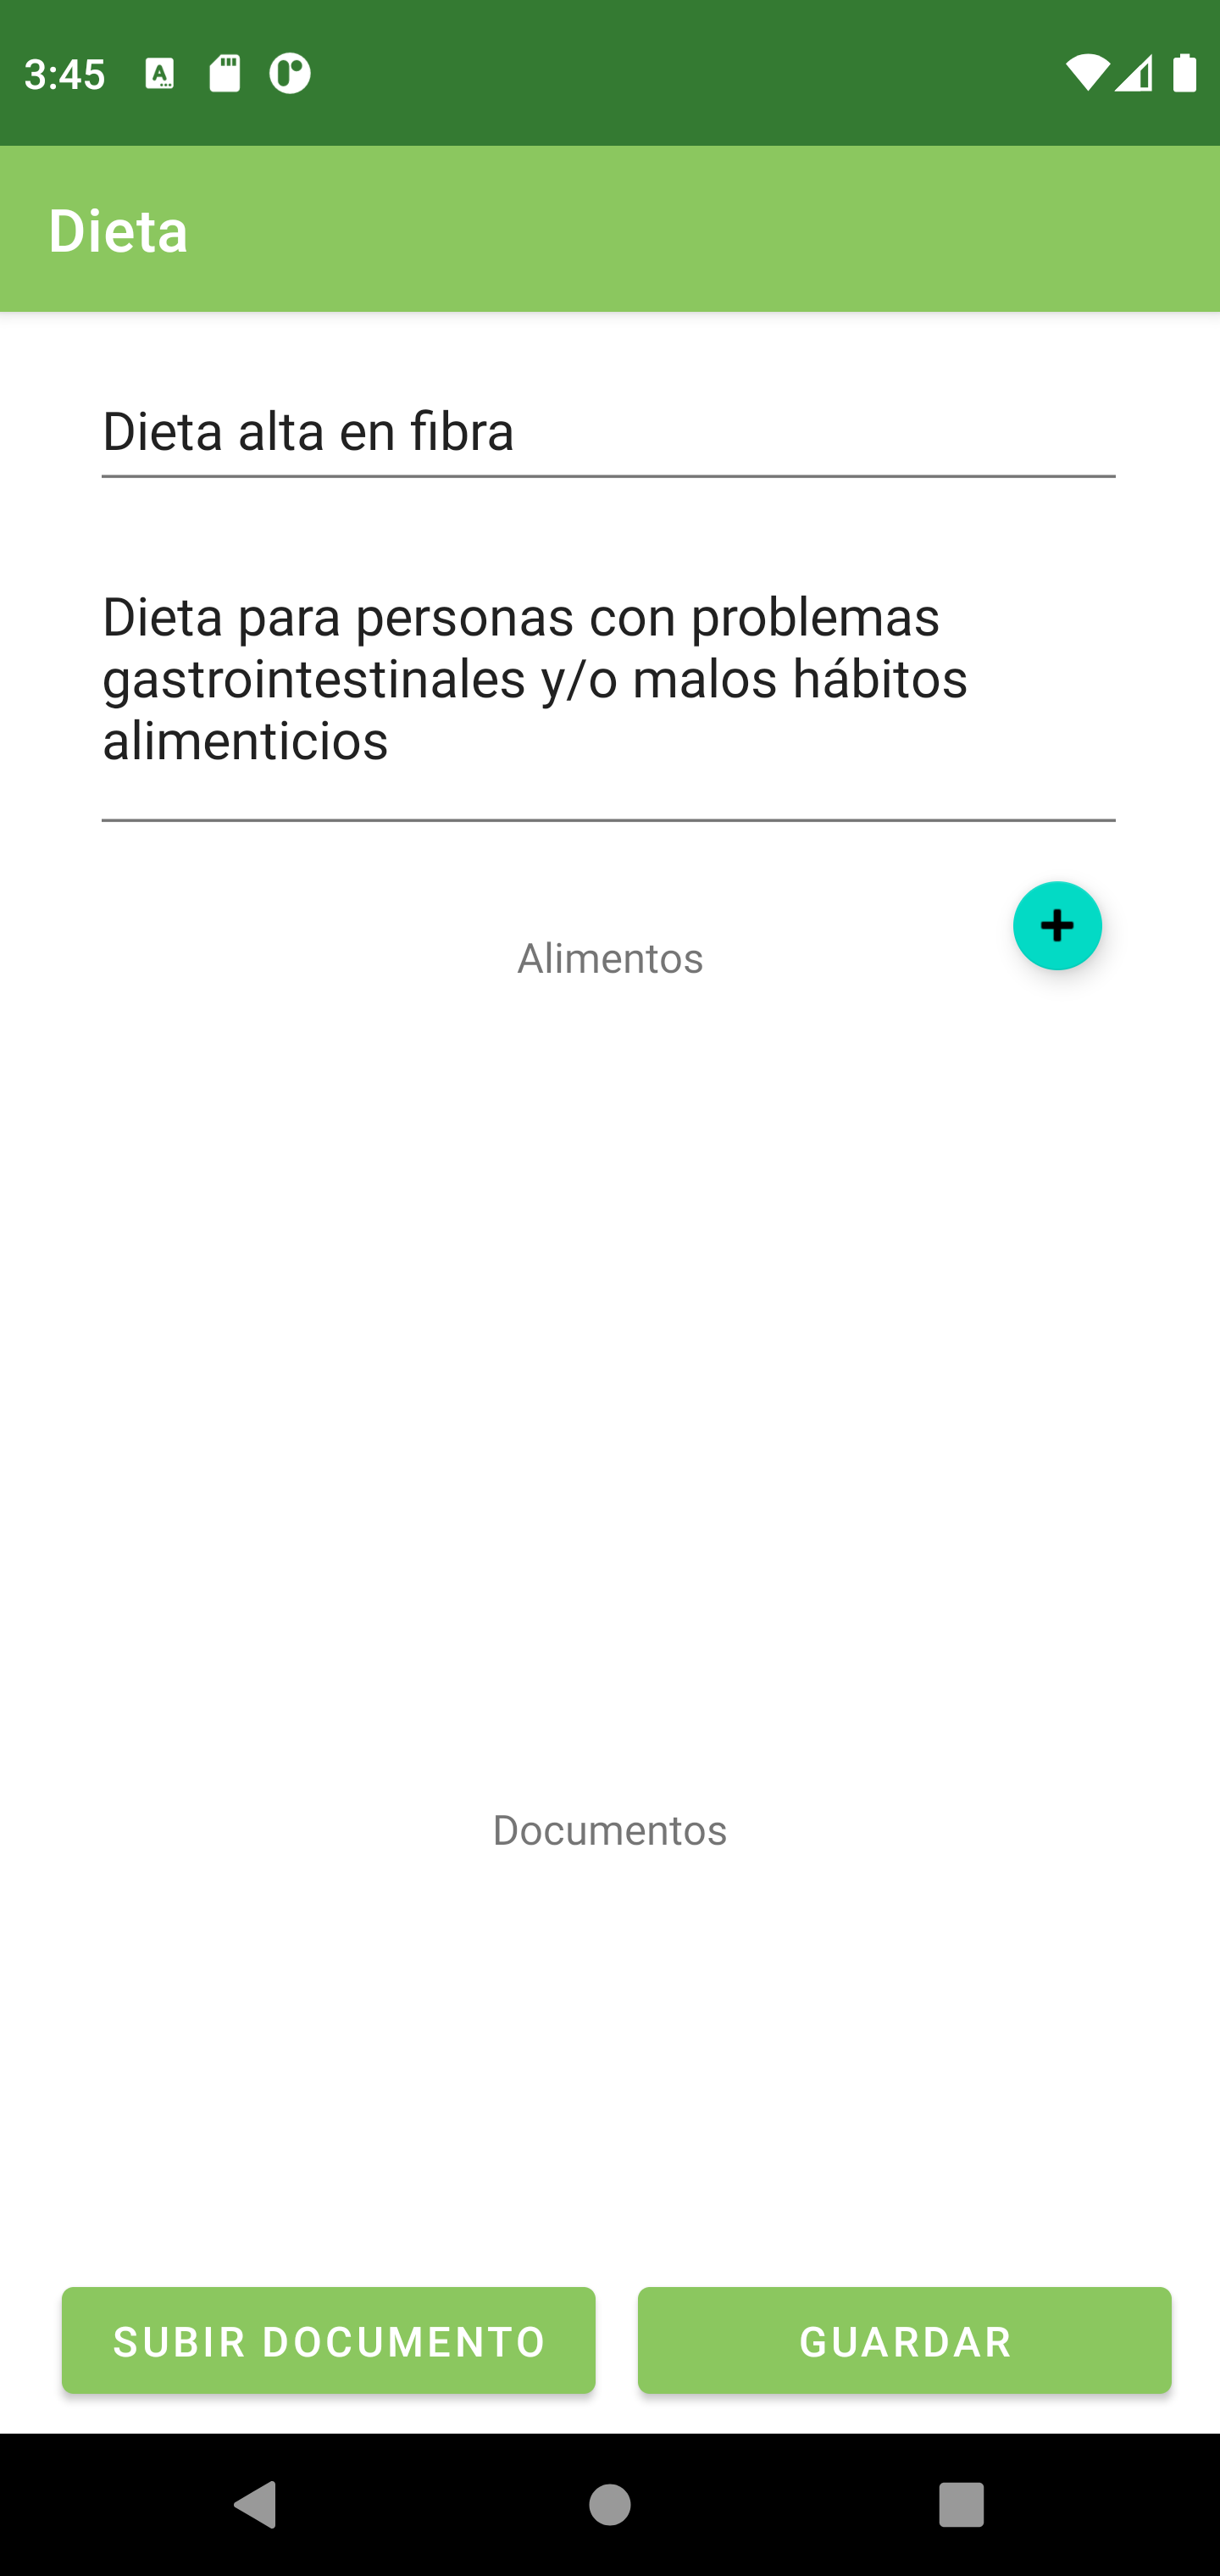
\includegraphics[width=0.5\textwidth]{Images/Capitulo7/editardieta.png}
        \caption{Vista de Editar Dieta}
    \label{fig:editardieta}
\end{figure}

Si se pulsa sobre el botón ``+`` se pueden añadir alimentos a la dieta. Se pueden añadir alimentos de dos formas diferentes, mediante el uso de la cámara o manualmente. (ver figura \ref{fig:addalim}).
\begin{figure}[H]
    \centering
    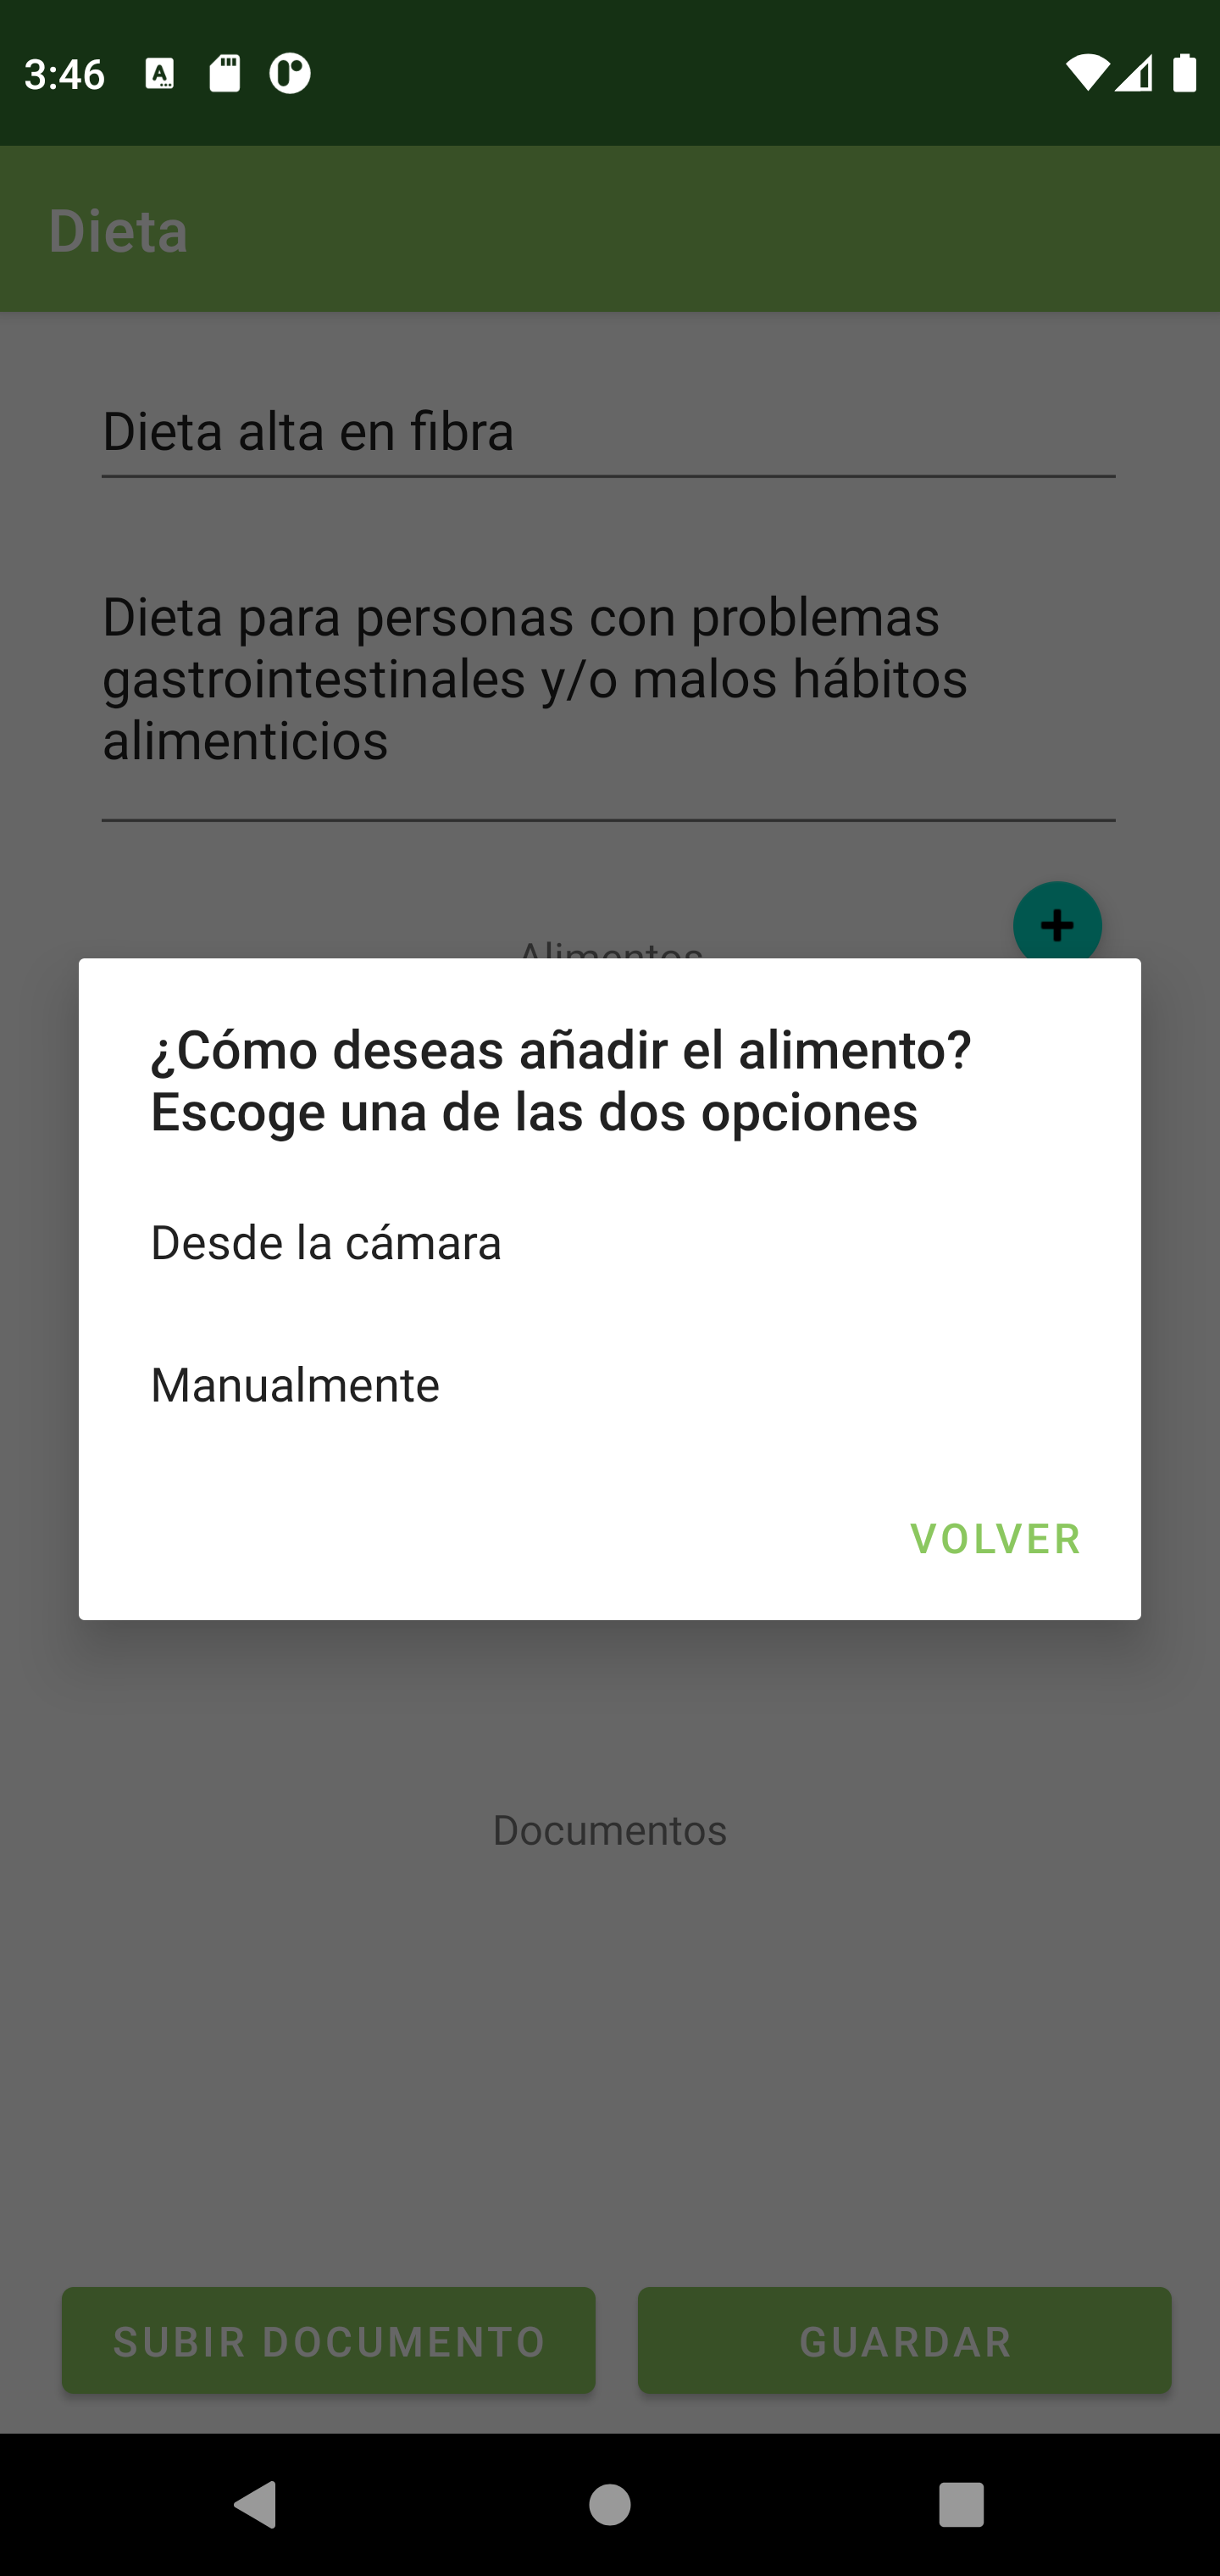
\includegraphics[width=0.5\textwidth]{Images/Capitulo7/addalim.png}
        \caption{Popup que aparece para elegir como añadir un alimento}
    \label{fig:addalim}
\end{figure}

Si se elige la opción manual (ver figura \ref{fig:manual}), se podrá añadir un alimento de dos maneras:  
\begin{enumerate}
    \item Con el código de barras.
    \item Introduciendo las características principales del alimento.
\end{enumerate}

\begin{figure}[H]
    \centering
    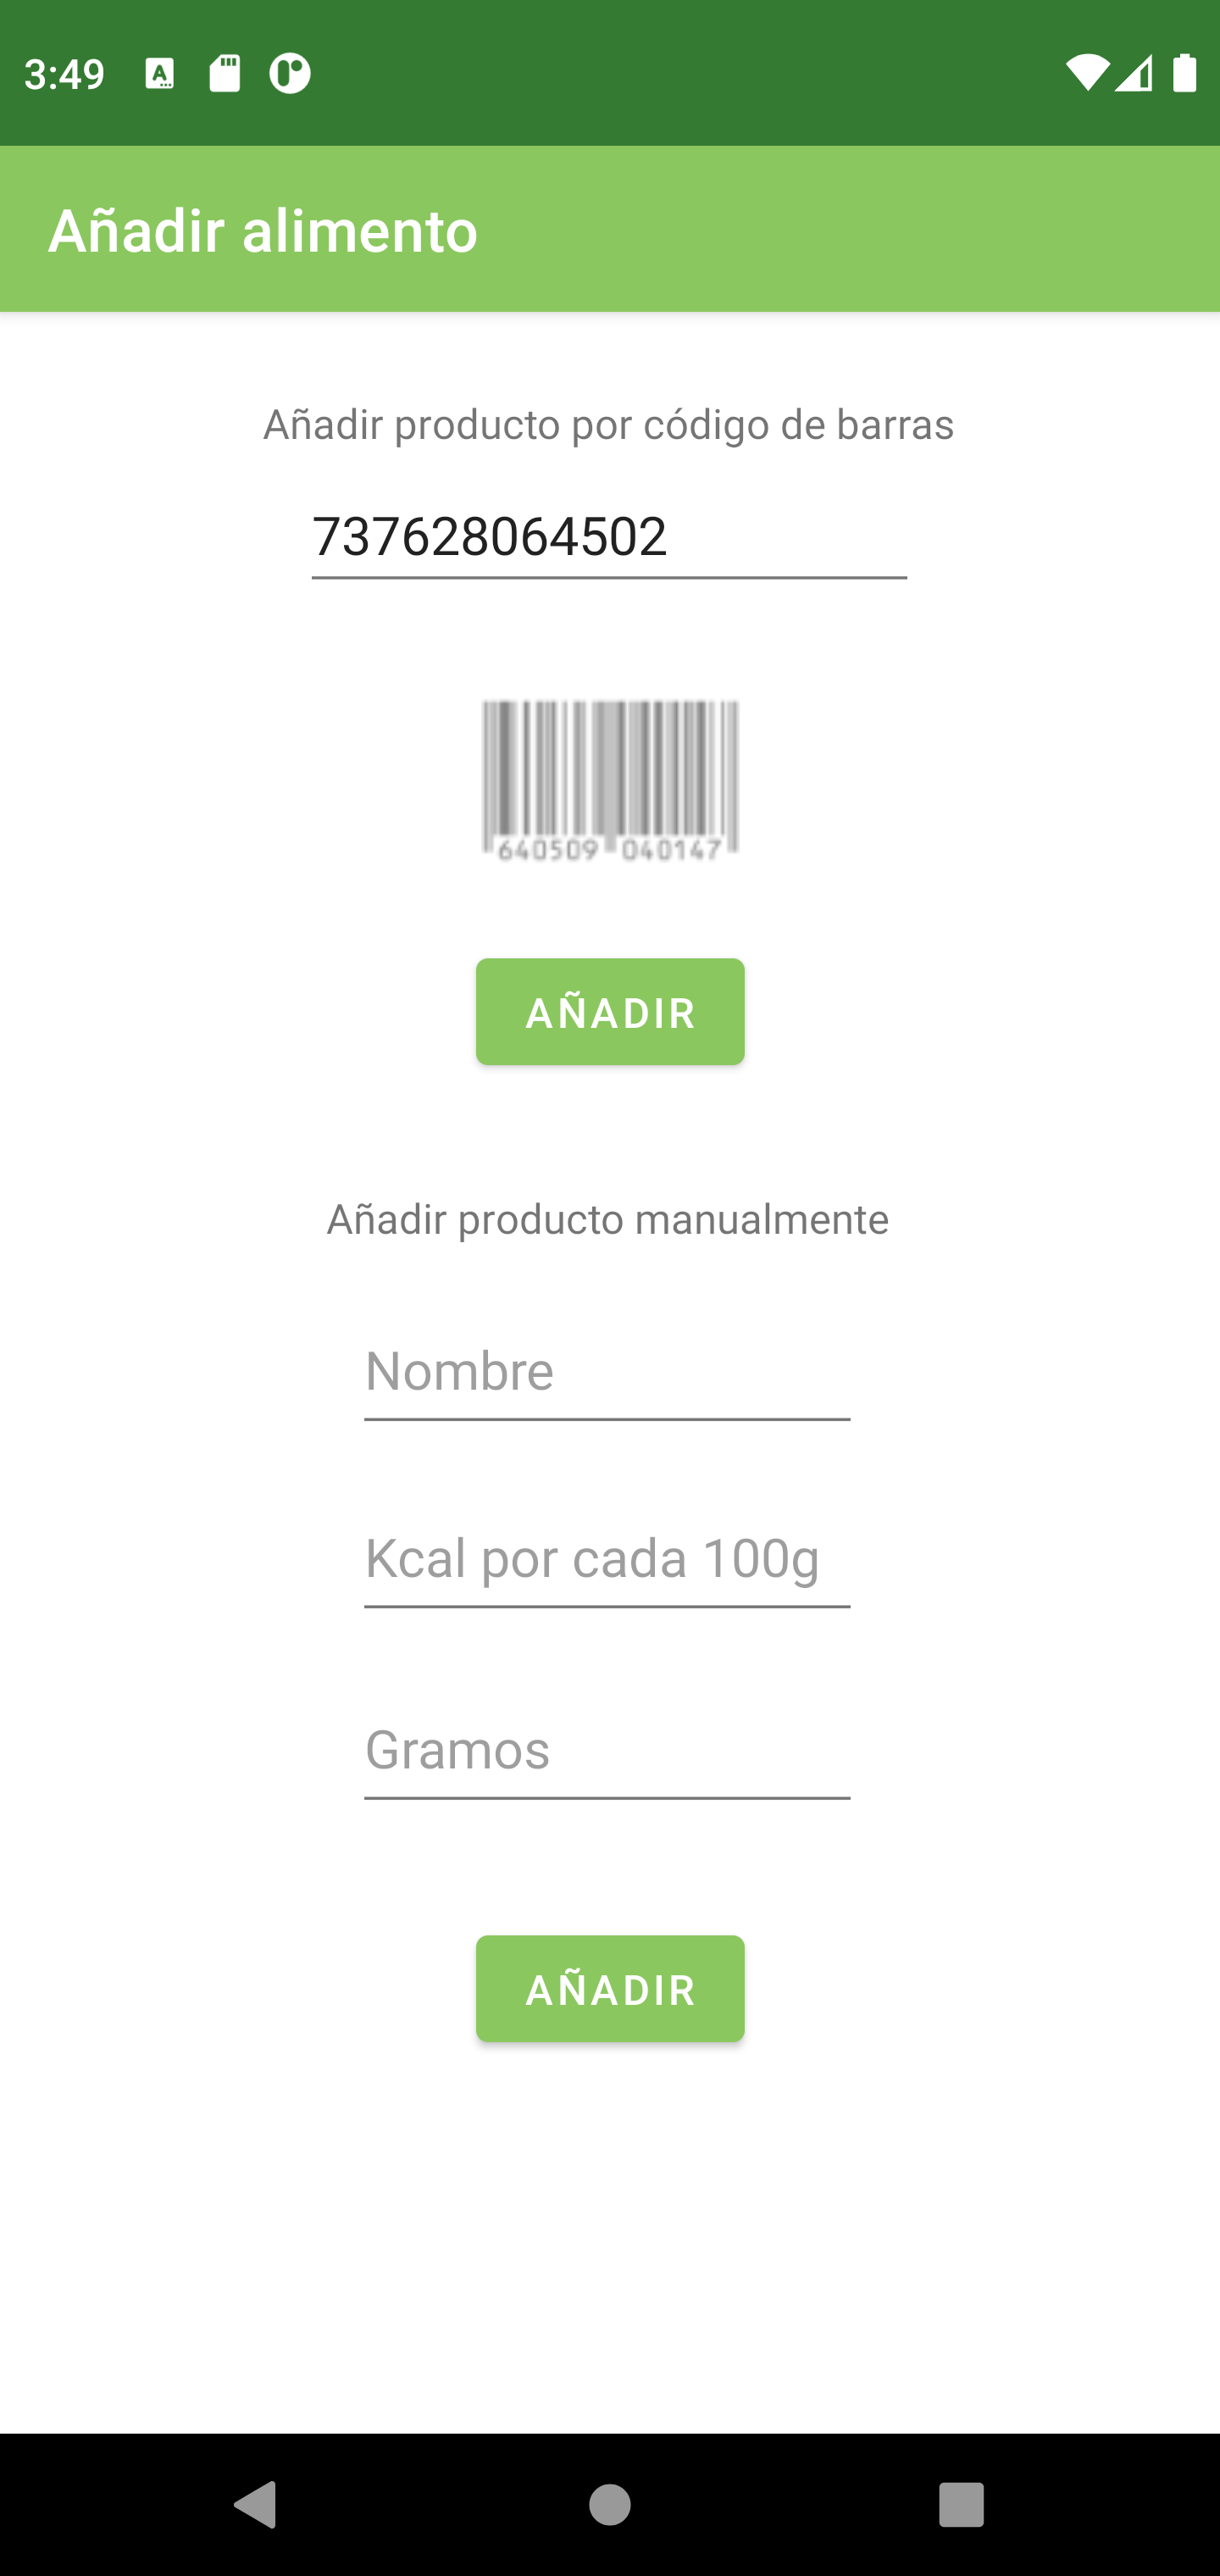
\includegraphics[width=0.5\textwidth]{Images/Capitulo7/manual.png}
        \caption{Vista de añadir un alimento manualmente}
    \label{fig:manual}
\end{figure}

Para añadir un alimento con el código de barras cuando se pulsa sobre el botón de añadir de la parte superior de la figura \ref{fig:manual}, se utiliza el método de la figura \ref{fig:barcode}
\begin{figure}[H]
    \centering
    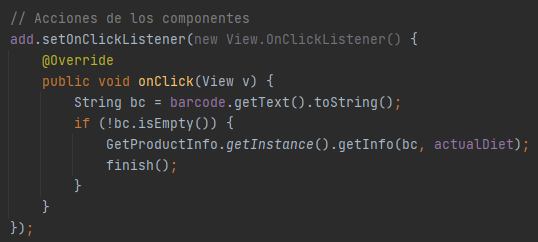
\includegraphics[width=\textwidth]{Images/Capitulo7/barcode.png}
        \caption{Código asociado a añadir alimentos mediante código de barras}
    \label{fig:barcode}
\end{figure}

La clase \texttt{GetProductInfo} (ver figura \ref{fig:productinfo}) es un Singleton, el cual realiza una petición al alias especial de la interfaz host del bucle invertido \cite{ip_emulator}.
\begin{figure}[H]
    \centering
    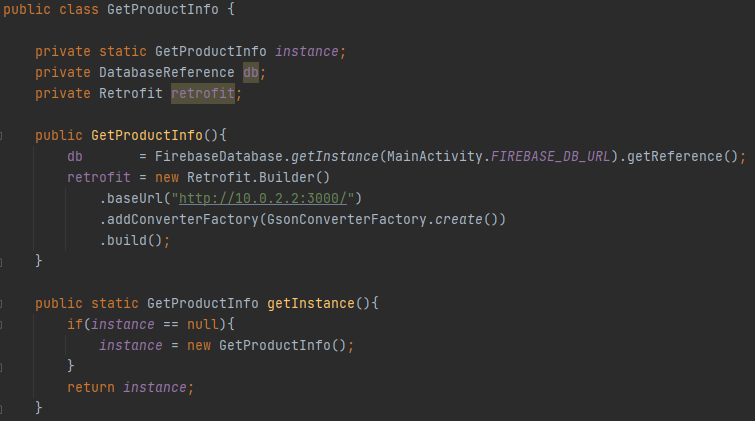
\includegraphics[width=\textwidth]{Images/Capitulo7/productinfo.png}
        \caption{Código de \texttt{GetProductInfo()}}
    \label{fig:productinfo}
\end{figure}
Para obtener la información del código de barras solicitado, se utiliza la API de Open Food Facts (ver figura \ref{fig:getinfo}).
\begin{figure}[H]
    \centering
    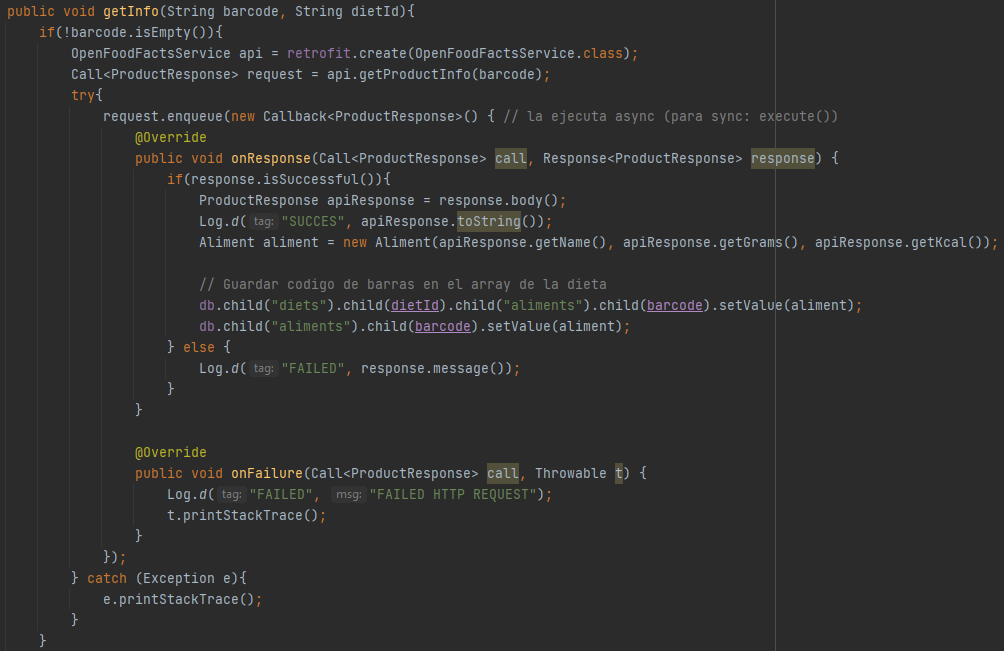
\includegraphics[width=\textwidth]{Images/Capitulo7/getinfo.png}
        \caption{Código de \texttt{getInfo()} dentro de \texttt{GetProductInfo()}}
    \label{fig:getinfo}
\end{figure}

Para añadir el alimento con el código de barras se ha utilizado Retrofit para poder manejar las peticiones HTTP sobre las diferentes API utilizadas en la aplicación.

Se definen las diferentes rutas sobre las que se va a hacer la petición HTTP al servidor de Node.js sobre la API OpenFoodFacts(ver figura \ref{fig:retrointerface}).
\begin{figure}[H]
    \centering
    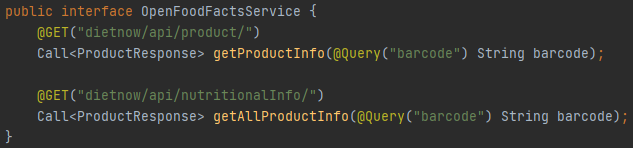
\includegraphics[width=\textwidth]{Images/Capitulo7/retrointerface.png}
        \caption{Código de la interfaz de la API OpenFoodFacts}
    \label{fig:retrointerface}
\end{figure}

Para ello se definen los \textit{endpoints} a los cuales Retrofit va a realizar las peticiones, en este caso para obtener las características principales de un producto y para obtener la información nutricional más específica de ese producto (ver figura \ref{fig:creacionservidor}).

\begin{figure}[H]
    \centering
    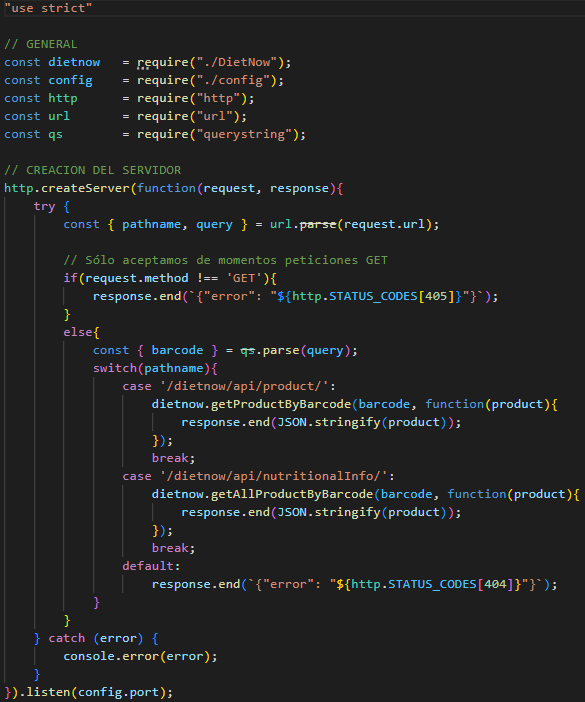
\includegraphics[width=\textwidth]{Images/Capitulo7/creacionservidor.png}
        \caption{Creación del servidor de node.js}
    \label{fig:creacionservidor}
\end{figure}

Posteriormente se hacen peticiones a la API de OpenFoodFacts para obtener la información del producto (ver figura \ref{fig:peticionapi}).

\begin{figure}[H]
    \centering
    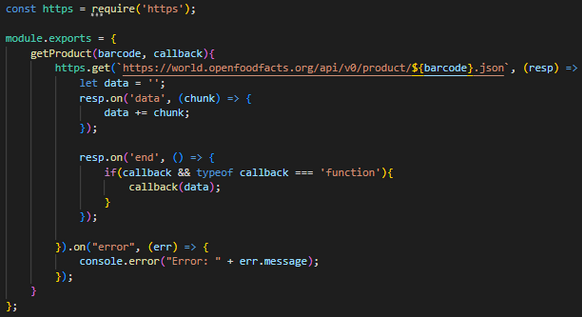
\includegraphics[width=\textwidth]{Images/Capitulo7/peticionapi.png}
        \caption{Código de la estructura de las peticiones a la API}
    \label{fig:peticionapi}
\end{figure}

La API de Open Food Facts devuelve un JSON con la respuesta a la petición realizada y en el código de la figura \ref{fig:returnapi} se formatea la información para obtener solo los campos que posteriormente se mostraran al usuario.

\begin{figure}[H]
    \centering
    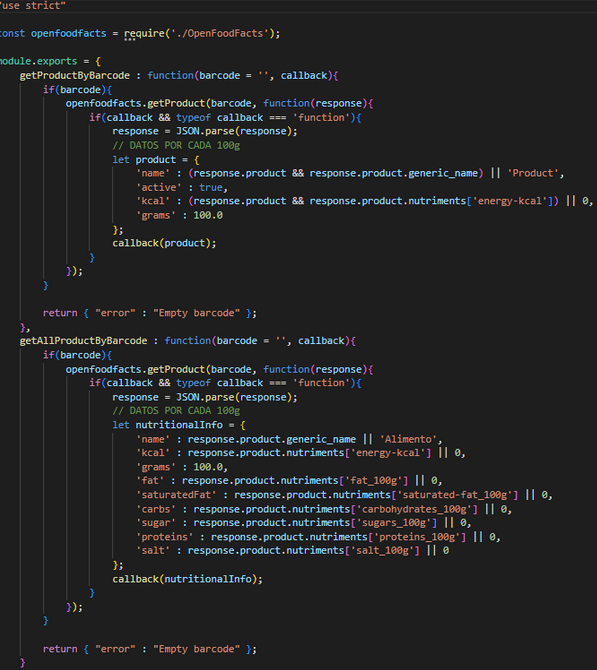
\includegraphics[width=\textwidth]{Images/Capitulo7/returnapi.png}
        \caption{Código del formateo de los JSON devueltos por OpenFoodFacts}
    \label{fig:returnapi}
\end{figure}

Para crear un alimento de forma manual introduciendo las principales características se utiliza el método mostrado en la figura \ref{fig:addmanual}

\begin{figure}[H]
    \centering
    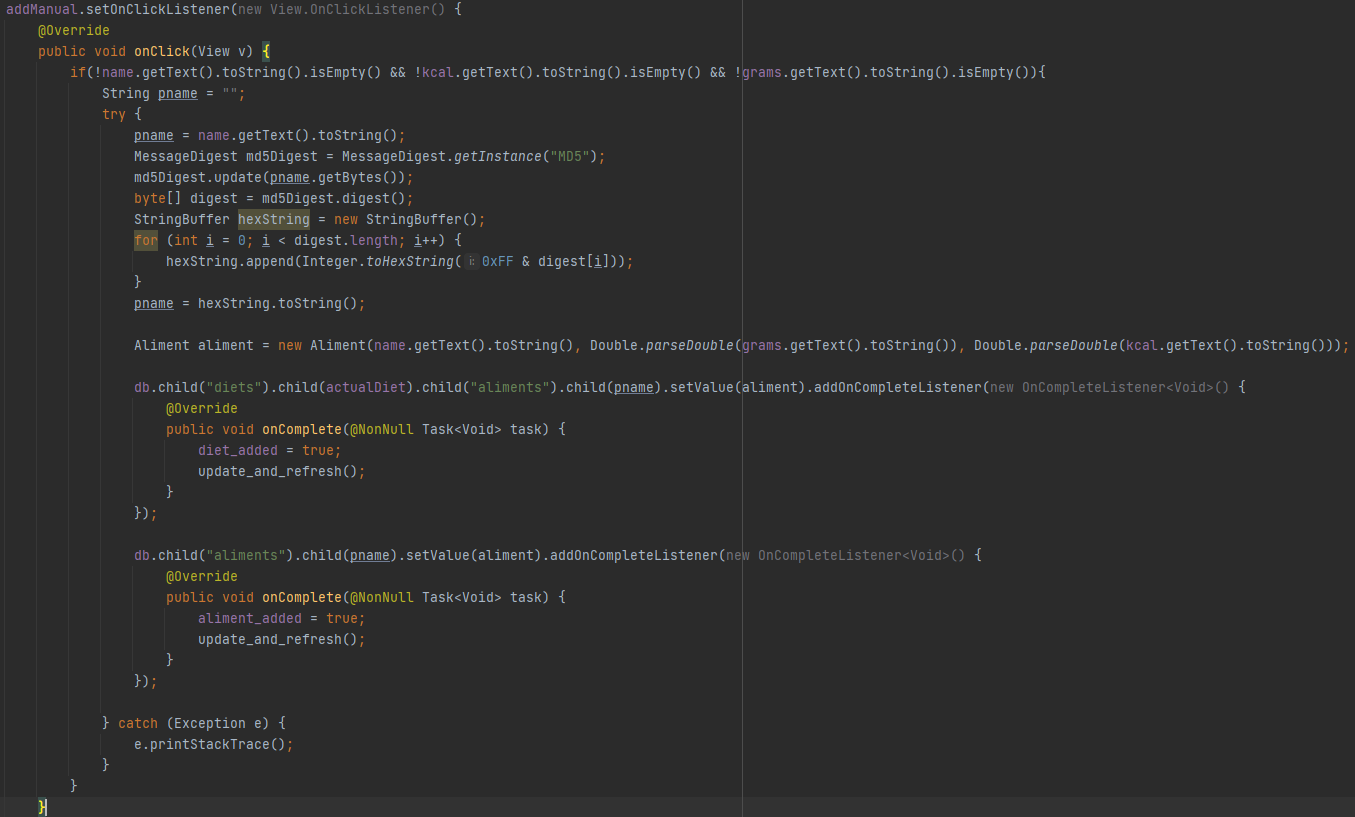
\includegraphics[width=\textwidth]{Images/Capitulo7/addmanual.png}
        \caption{Código del método que añade alimento de forma manual}
    \label{fig:addmanual}
\end{figure}

Se genera un código MD5 para poder insertar el alimento a la base de datos con el código como clave principal.

Para añadir un alimento utilizando la cámara (ver figura \ref{fig:camara_action}), se realiza mediante la actividad \texttt{CameraActivity} que implementa un escáner \cite{code_scanner} que al detectar un código de barras identifica el número y realiza la consulta a OpenFoodFacts con el código. En la figura \ref{fig:cameraact1} se ilustra el código de la \texttt{CameraActivity}.

\begin{figure}[H]
    \centering
    \includegraphics[width=0.5\textwidth]{Images/Annexes/añadir_alimentos_camara.jpg}
    \caption{Añadir alimento mediante el uso de la cámara}
    \label{fig:camara_action}
\end{figure}

\begin{figure}[H]
    \centering
    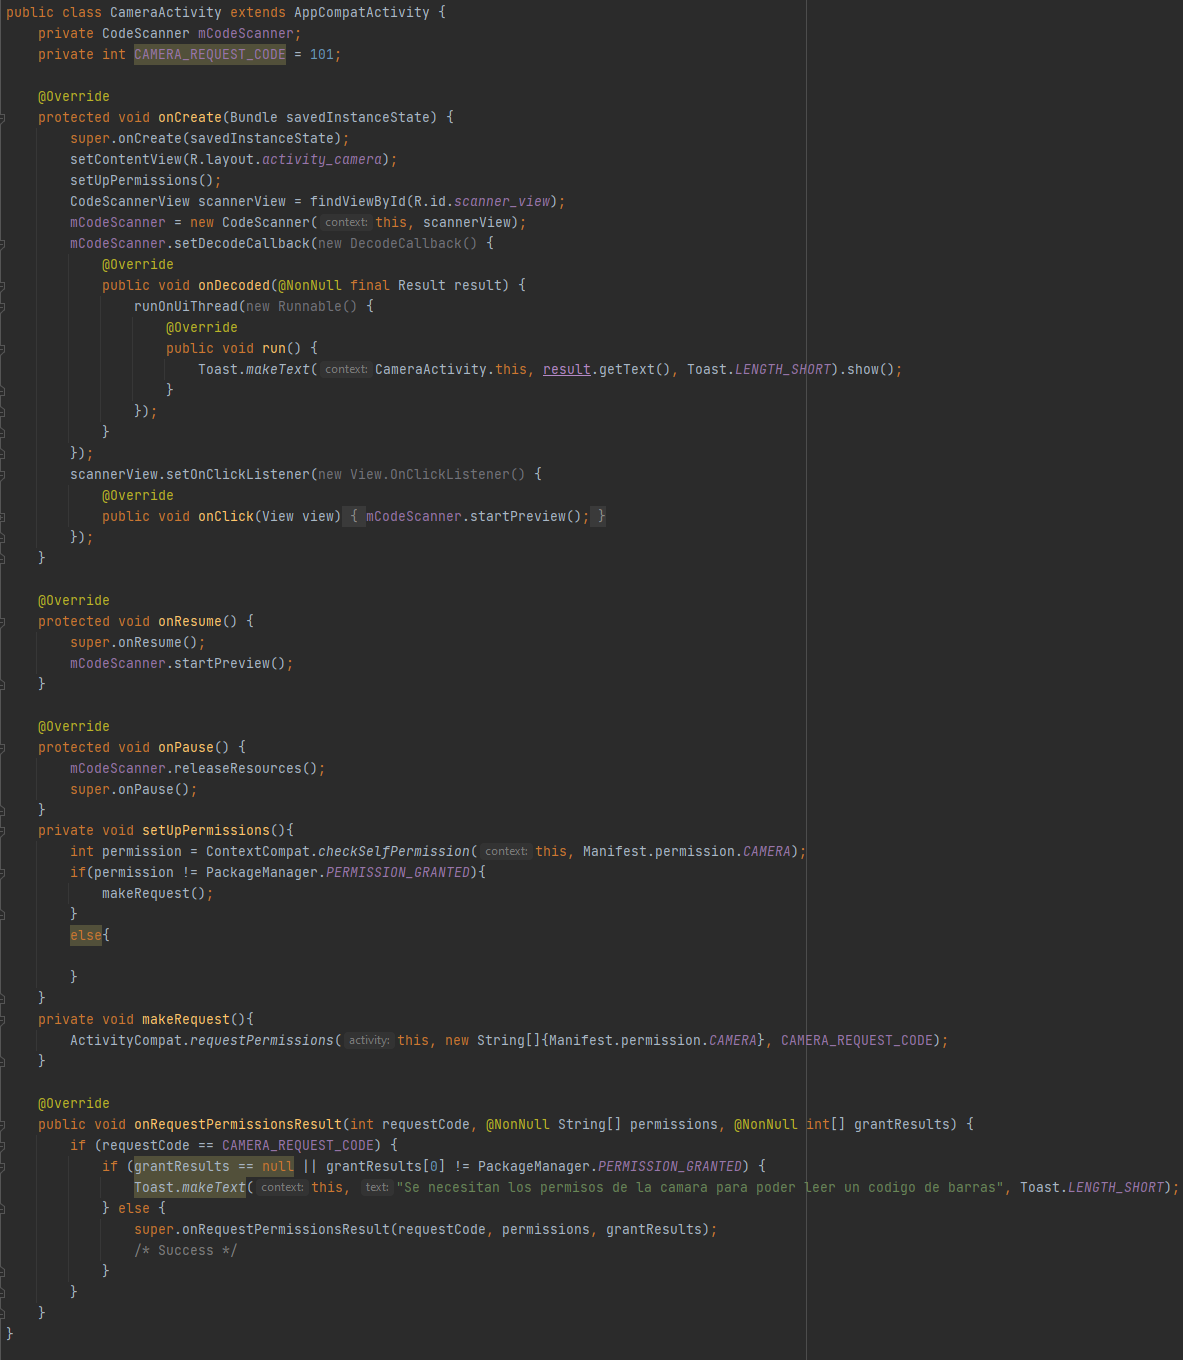
\includegraphics[width=\textwidth]{Images/Capitulo7/cameraact1.png}
    \caption{Código de \texttt{CameraActivity}}
    \label{fig:cameraact1}
\end{figure}

Para añadir un documento se utiliza el método de la figura \ref{fig:getdocfrom} que abre los archivos del teléfono para poder seleccionar un documento que este almacenado en el dispositivo (ver figura \ref{fig:archivos}).

\begin{figure}[H]
    \centering
    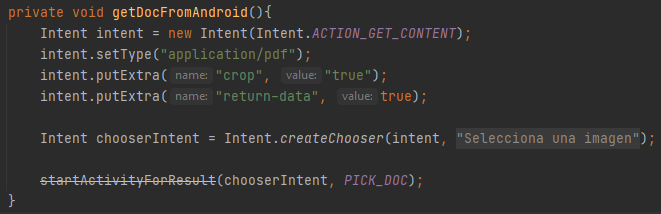
\includegraphics[width=\textwidth]{Images/Capitulo7/getdocfrom.png}
        \caption{Código del método abre los archivos del teléfono para obtener los documentos}
    \label{fig:getdocfrom}
\end{figure}

\begin{figure}[H]
    \centering
    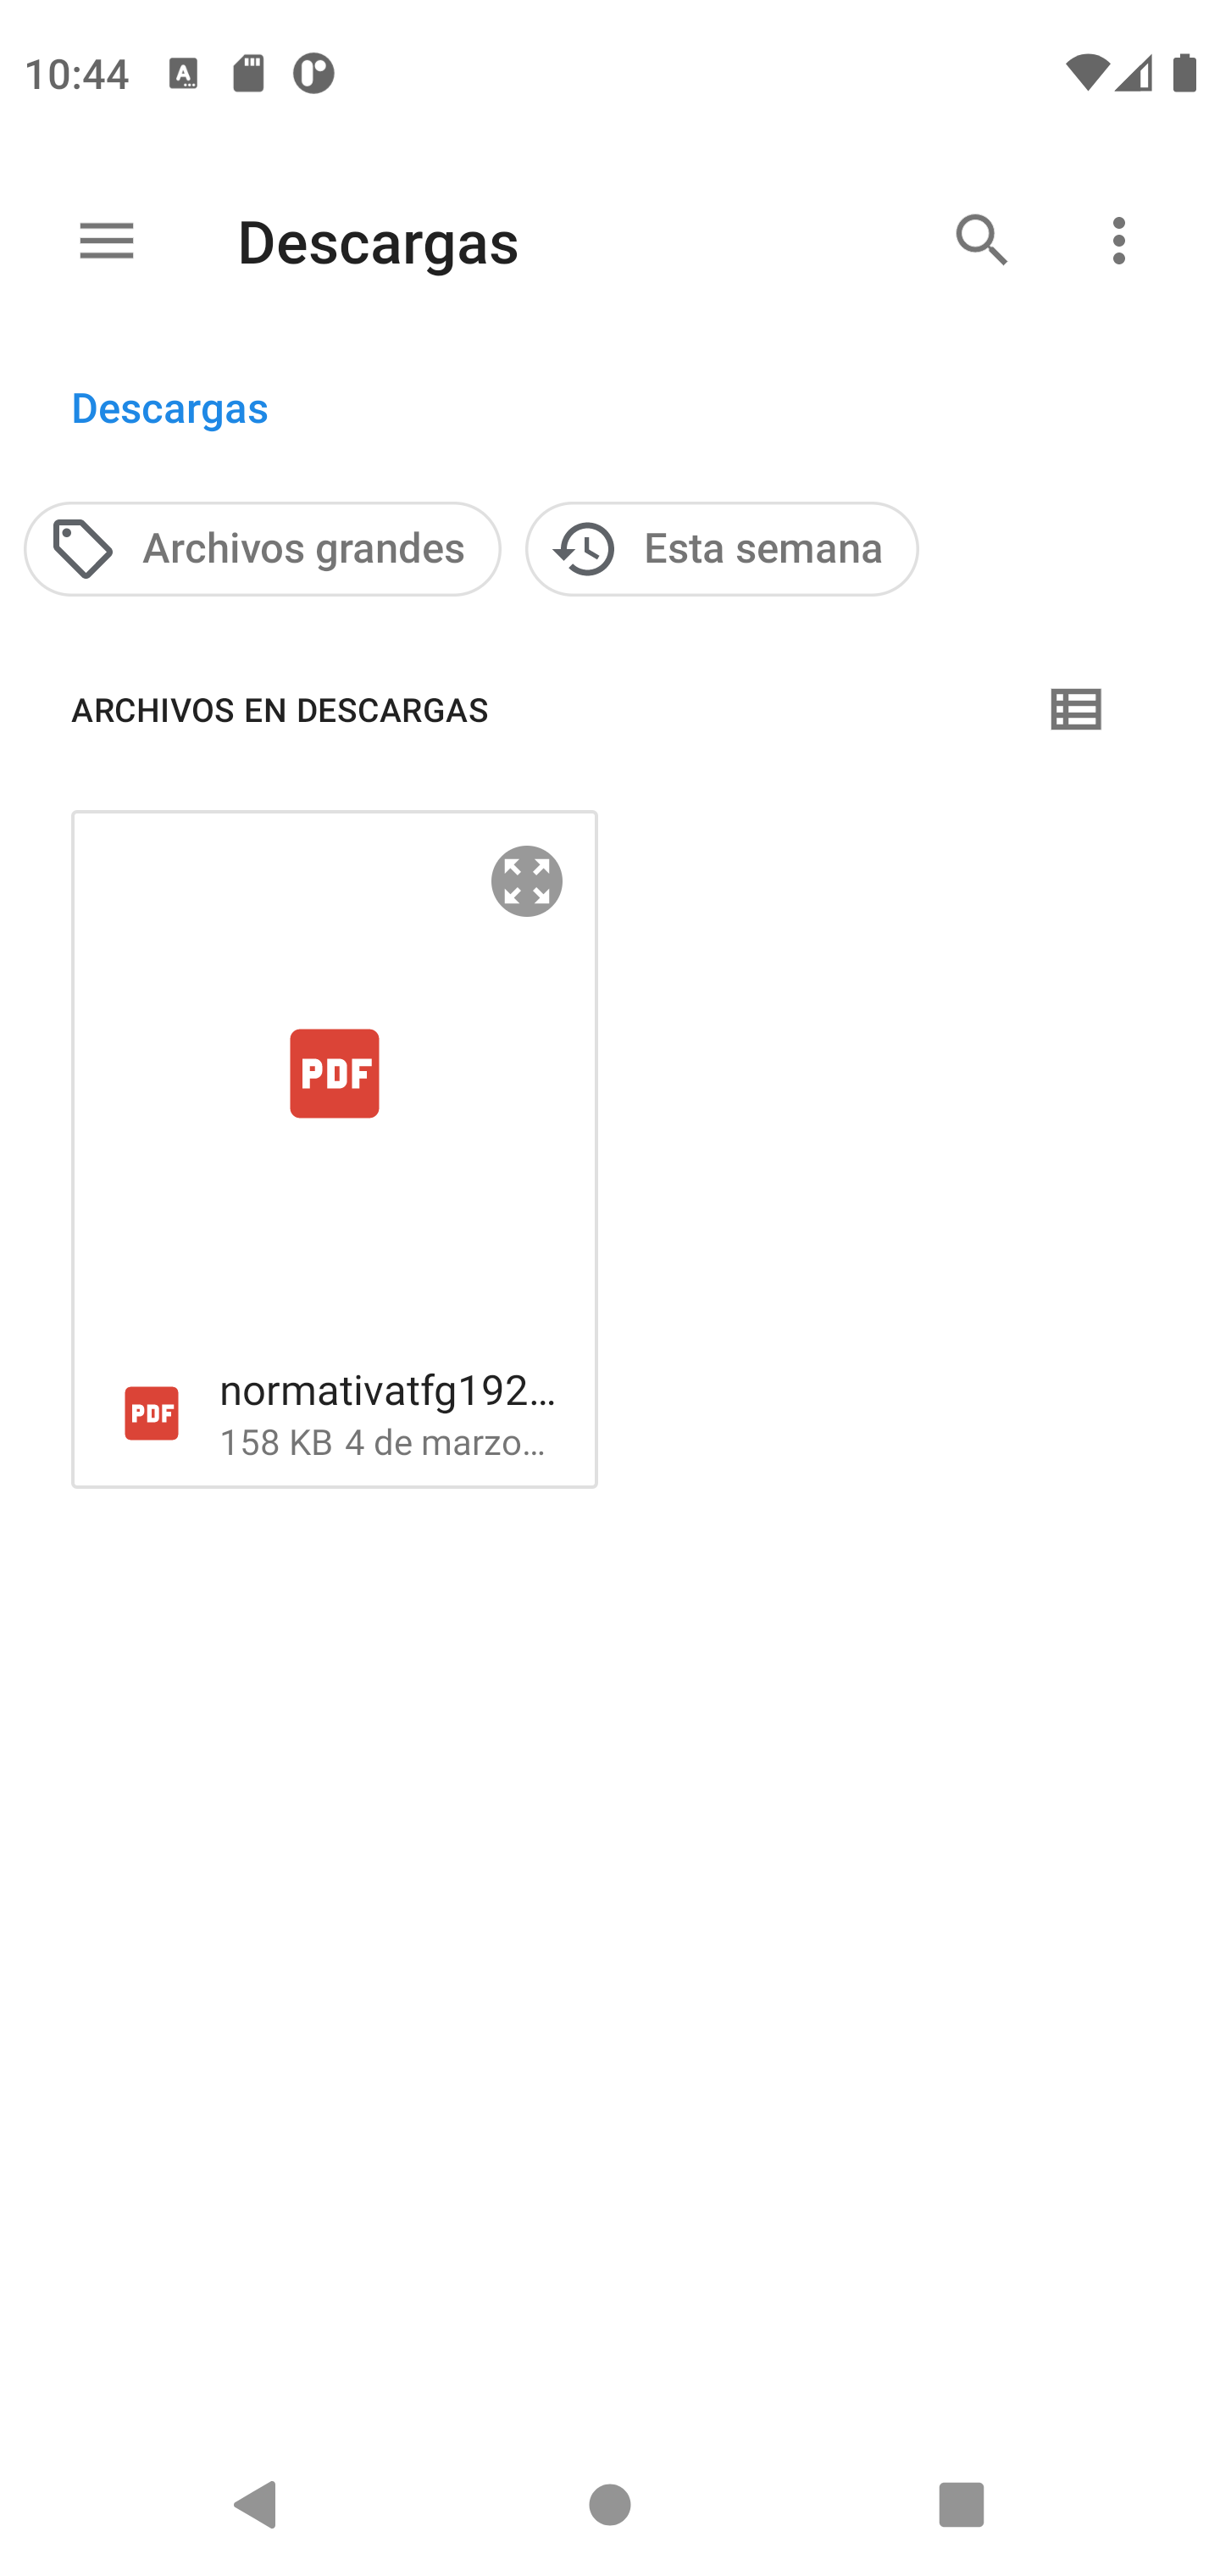
\includegraphics[width=0.5\textwidth]{Images/Capitulo7/archivos.png}
        \caption{Vista del almacenamiento del dispositivo}
    \label{fig:archivos}
\end{figure}

\subsection{Dieta actual}
Esta vista ofrece al usuario toda la información relativa a la dieta que está siguiendo, en dicha vista se puede visualizar la cantidad consumida de cada alimento a lo largo de la semana, pudiendo introducir la cantidad consumida en el día actual. Además permite valorar la dieta por medio de un me gusta o no me gusta, así como realizar un comentario sobre la dieta, el cual será visto por todos los usuarios.

La funcionalidad de este caso de uso se realiza en la la actividad \texttt{DietInfoActivity} (ver figura \ref{fig:dietinfo}).

\begin{figure}[H]
    \centering
    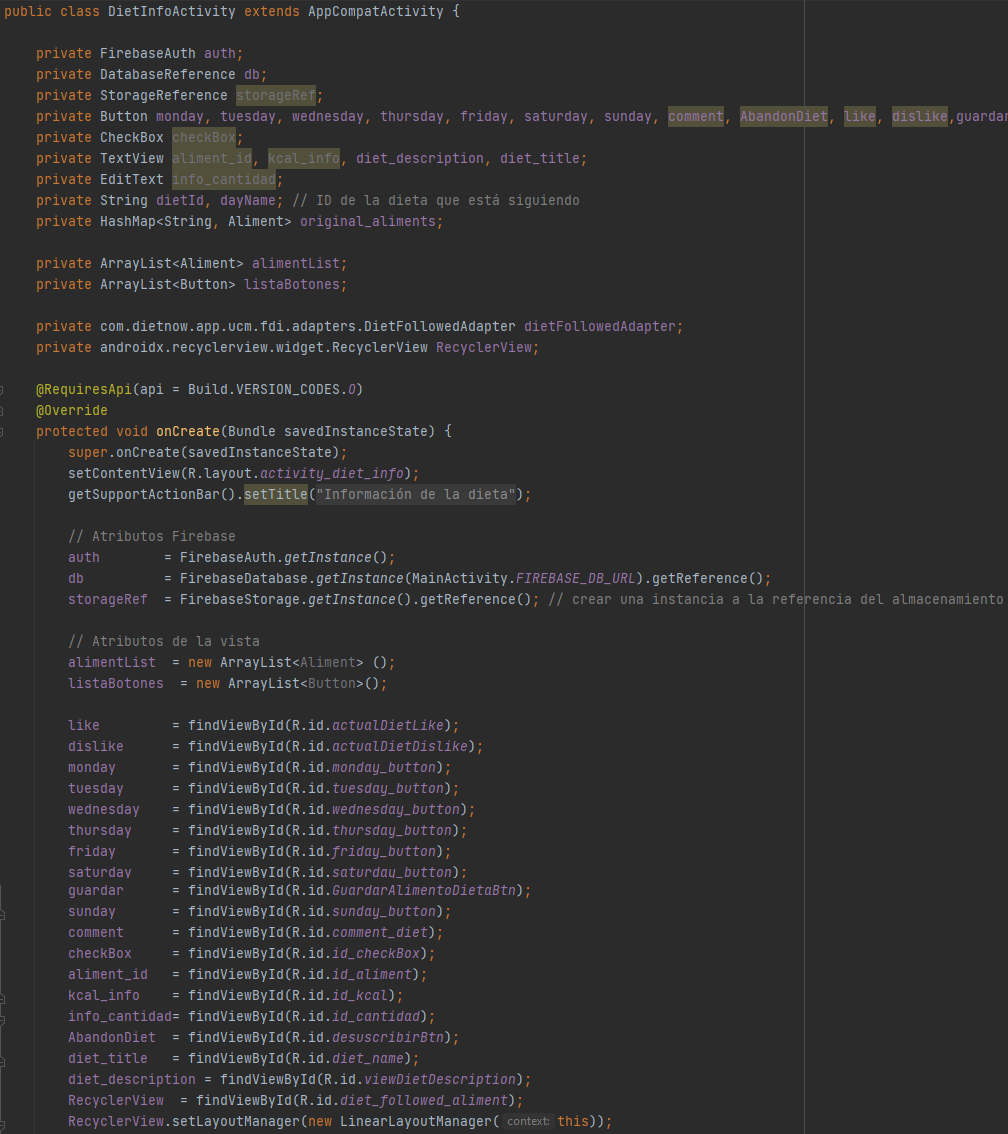
\includegraphics[width=\textwidth]{Images/Capitulo7/dietinfo.png}
        \caption{Código de DietInfoActivity}
    \label{fig:dietinfo}
\end{figure}

En el método \texttt{onCreate()} se inicializan las referencias de Realtime Database, Authentication de Firebase y de los diferentes componentes de la vista ``Información de la dieta`` (ver figura \ref{fig:infodieta}).

\begin{figure}[H]
    \centering
    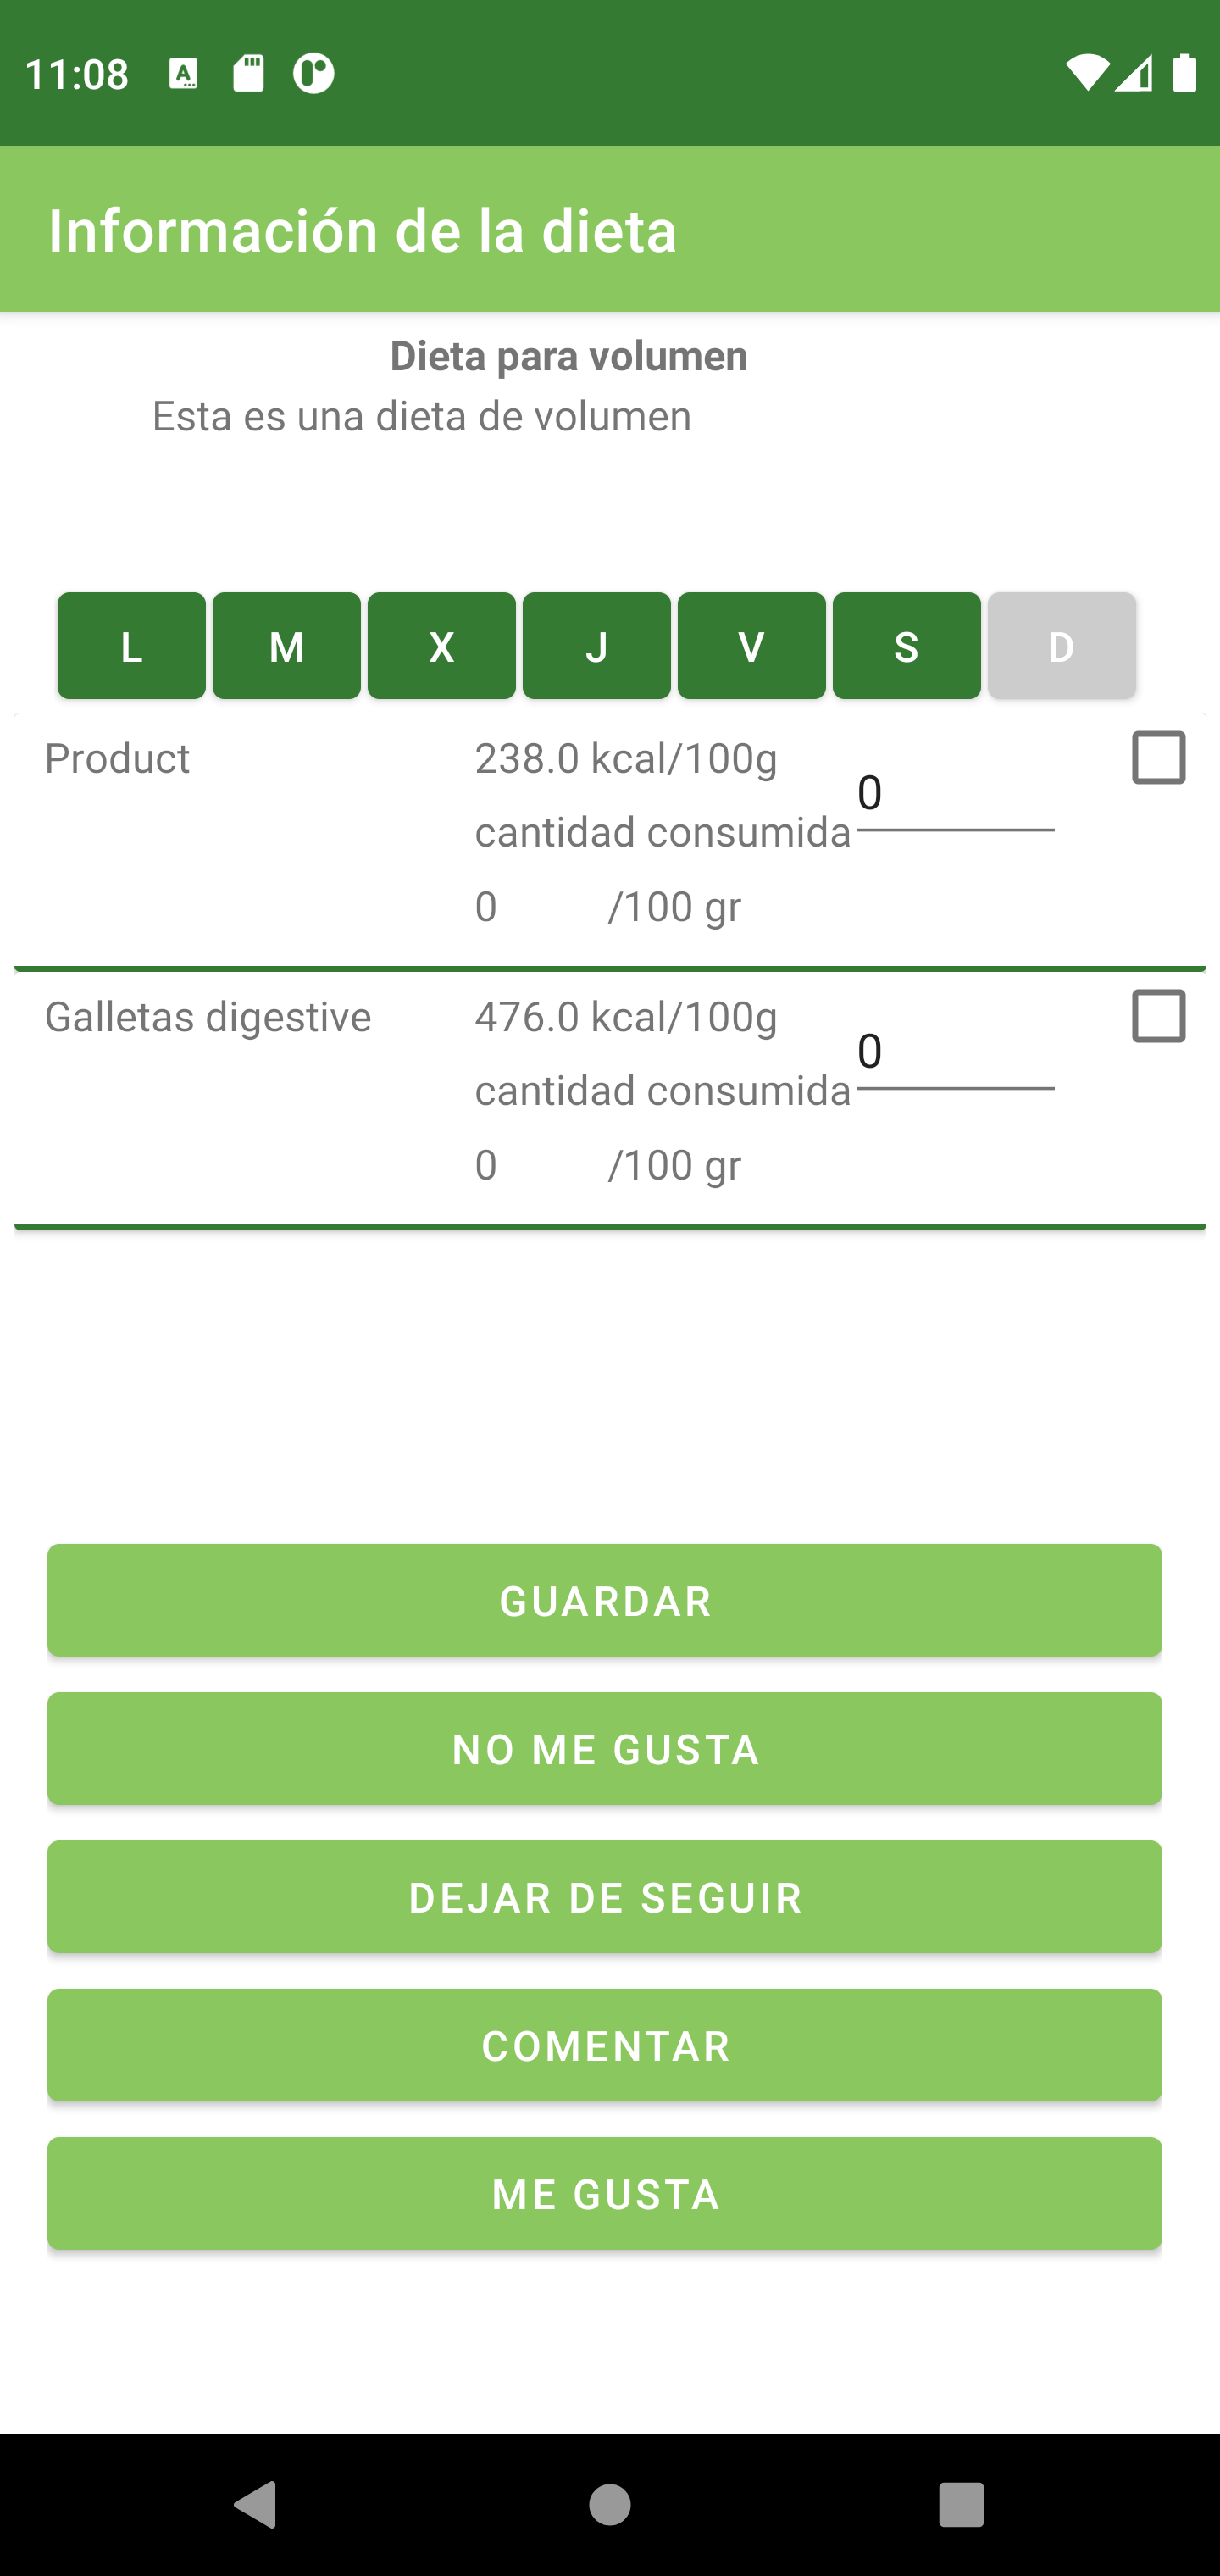
\includegraphics[width=0.5\textwidth]{Images/Capitulo7/infodieta.png}
    \caption{Vista Información de la dieta}
    \label{fig:infodieta}
\end{figure}

Para obtener la información de las calorías consumidas durante el día actual se utiliza el método \texttt{getAliments()} (ver figura \ref{fig:getaliments}).

\begin{figure}[H]
    \centering
    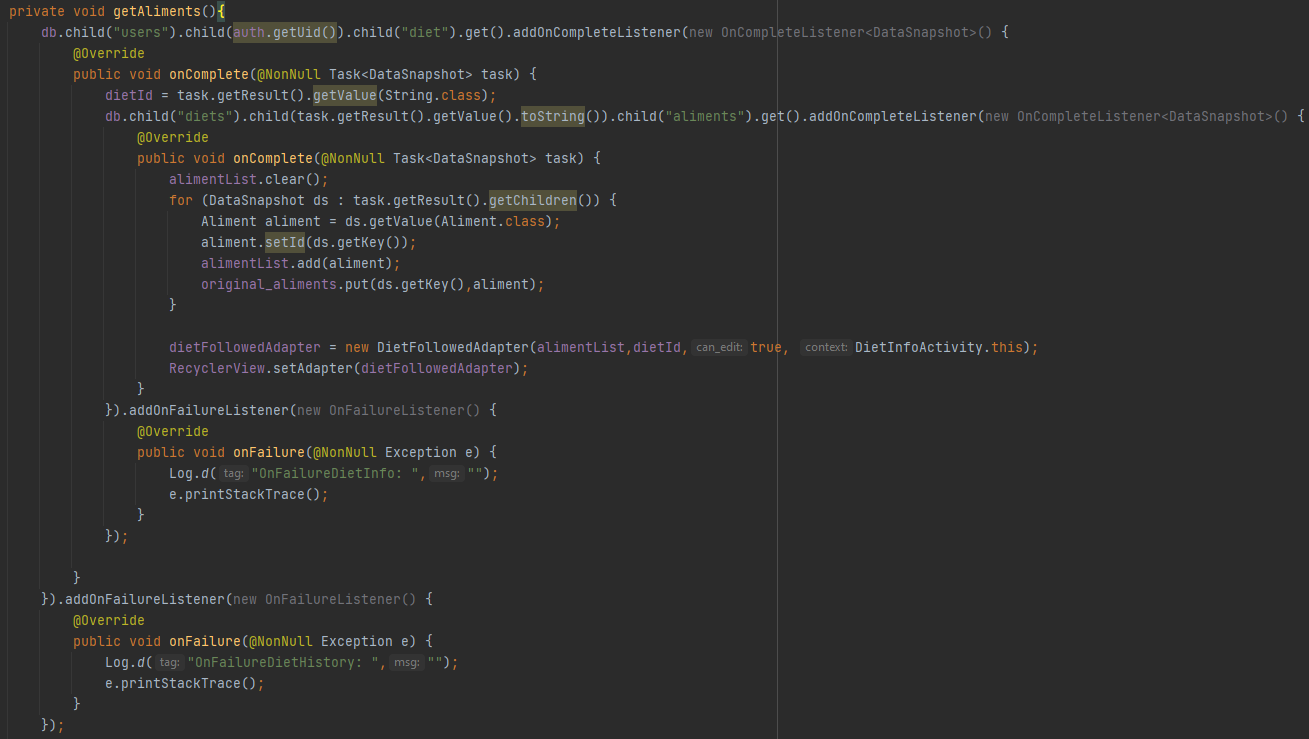
\includegraphics[width=\textwidth]{Images/Capitulo7/getaliments.png}
    \caption{Código del método \texttt{getAliments()}}
    \label{fig:getaliments}
\end{figure}

En dicho método se carga la información relativa a la dieta actual y se rellena la lista de alimentos para que el \texttt{DietFollowAdapter} muestre dinámicamente los alimentos de la dieta (ver figura \ref{fig:dietfollowedadapter}).

\begin{figure}[H]
    \centering
    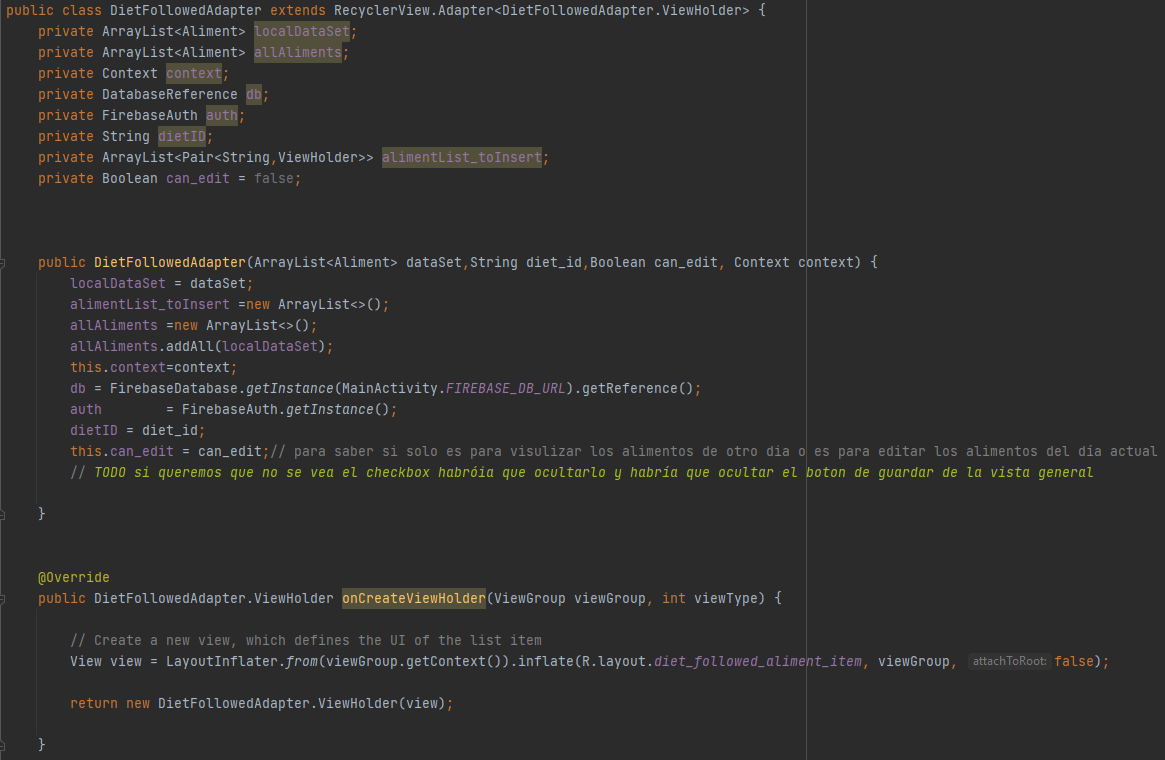
\includegraphics[width=\textwidth]{Images/Capitulo7/dietfollowedadapter.png}
    \caption{Código del adapter \texttt{DietFollowAdapter()}}
    \label{fig:dietfollowedadapter}
\end{figure}

En el método \texttt{OnBindViewHolder()} del adaptador (ver figura \ref{fig:onbindview}), si se puede editar la cantidad de gramos consumidos por el usuario de un alimento de la dieta, es decir, si se ha seleccionado en la vista el día actual, se consulta la tabla ``\texttt{diet\_history}`` de Realtime Database para comprobar si se ha consumido alguna cantidad del alimento seleccionado previamente durante el día actual, para ir guardando ese alimento en un mapa e ir actualizando el número de gramos consumidos de ese alimento.
En el caso de que no se pueda editar, es decir no se ha seleccionado el día actual, se actualiza la vista con la cantidad consumida de cada alimento el día seleccionado.

\begin{figure}[H]
    \centering
    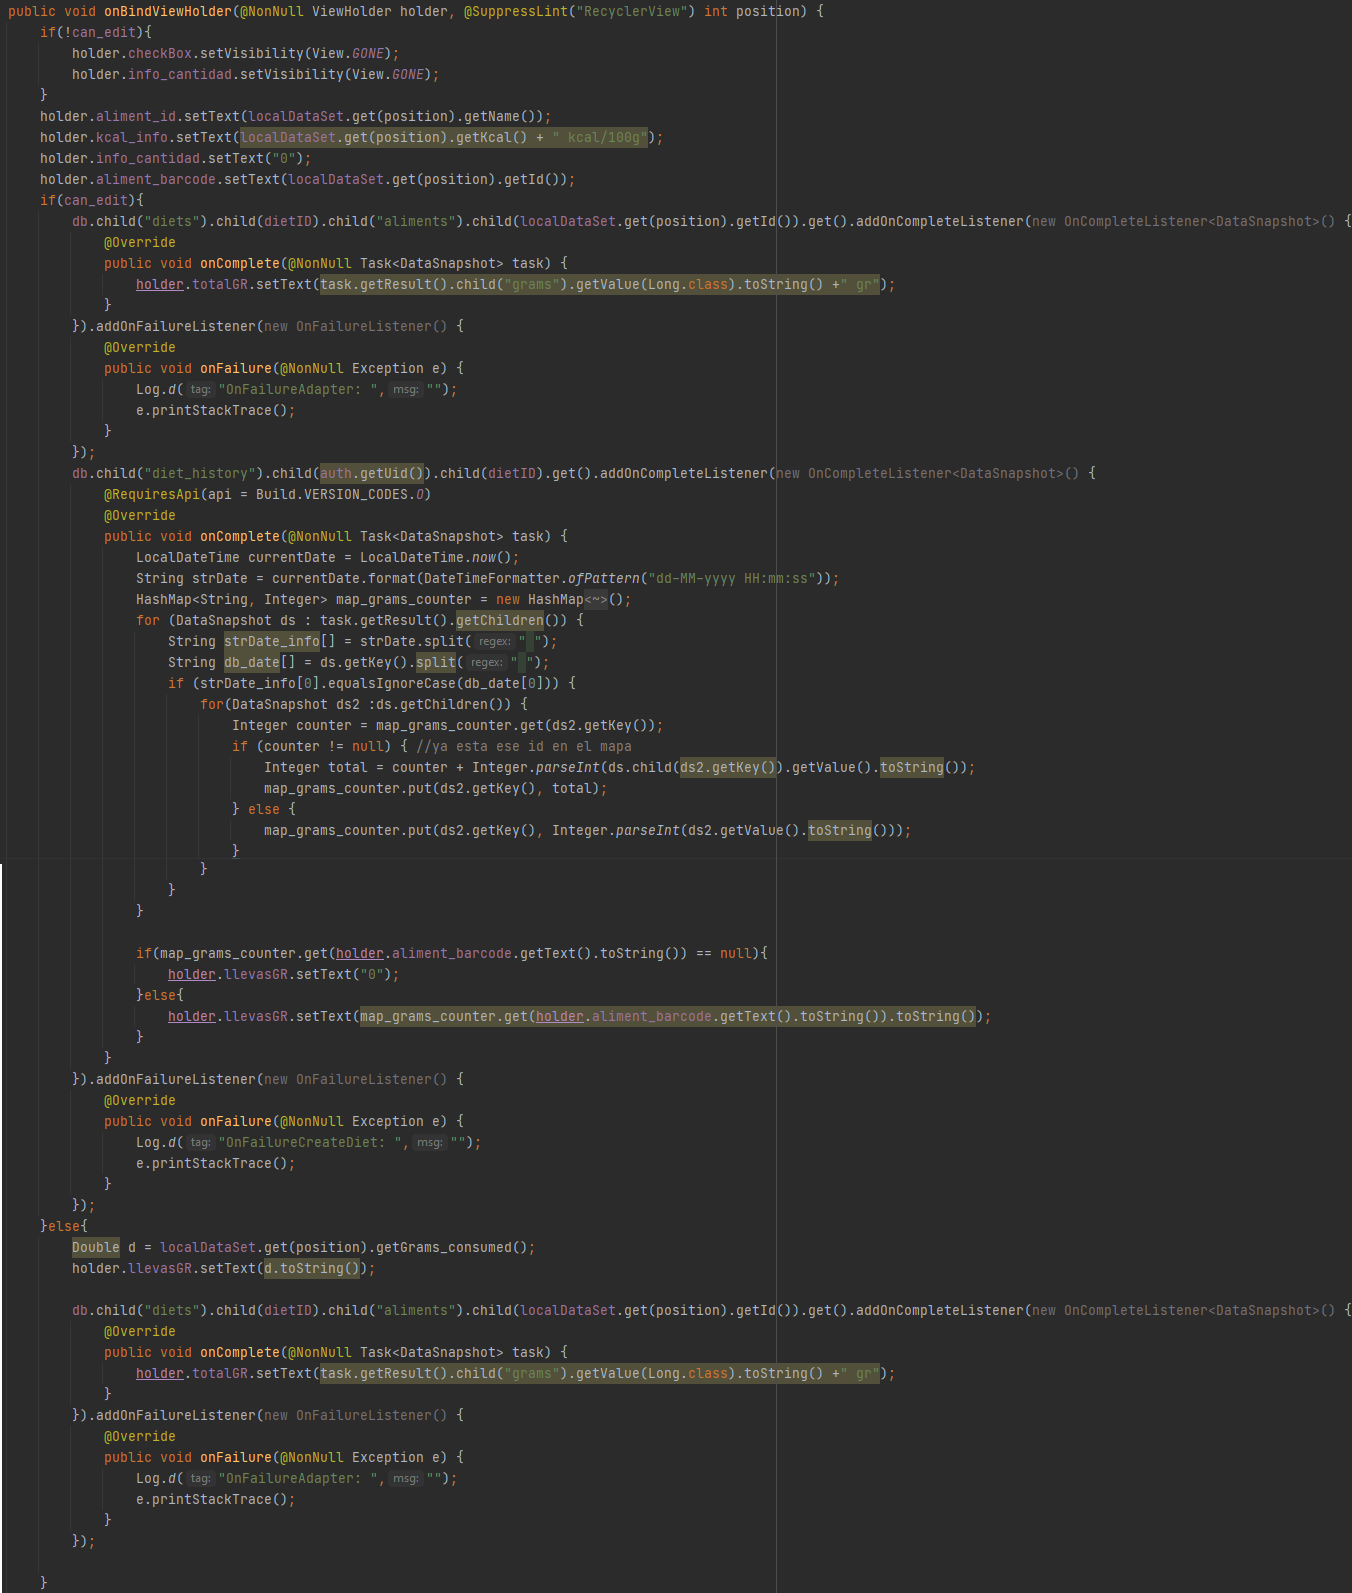
\includegraphics[width=\textwidth]{Images/Capitulo7/onbindview.png}
    \caption{Código de \texttt{OnBindViewHolder()}}
    \label{fig:onbindview}
\end{figure}

Cuando el usuario quiere actualizar la cantidad consumida de un alimento de la dieta durante el día actual, debe rellenar cuadro de texto (elemento número 1 en la figura \ref{fig:modinfodieta}) y posteriormente pulsar sobre el \textit{checkBox} (elemento número 2 en la figura \ref{fig:modinfodieta}) cuyo código está ilustrado en la figura \ref{fig:alimentlistto}, para indicar la cantidad de gramos de cada alimento a insertar. Desde el \texttt{DietFollowedAdapter()} se inserta en una lista de pares el código del alimento a introducir y la información relativa a ese alimento.

\begin{figure}[H]
    \centering
    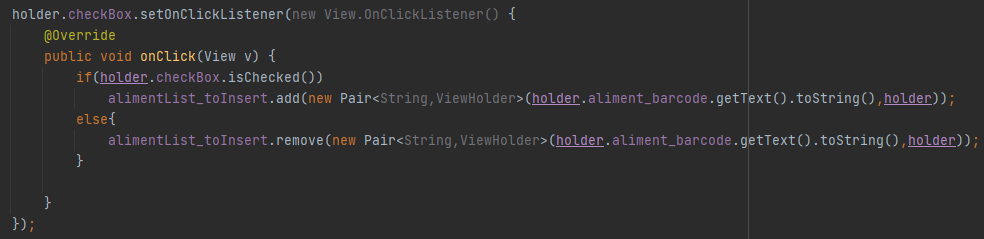
\includegraphics[width=\textwidth]{Images/Capitulo7/alimentlistto.png}
    \caption{Código del \textit{listener} del \textit{checkBox} de cada alimento}
    \label{fig:alimentlistto}
\end{figure}

Después de haber introducido los gramos consumidos de cada alimento y haber pulsado sobre el \textit{checkBox} en cada uno de los alimentos que se quieren actualizar, desde la actividad \texttt{DietInfoActivity()}, tras pulsar sobre el botón de guardar (elemento número 3 en la figura \ref{fig:modinfodieta}) de la vista ``Información de la dieta`` se actualizan los datos en la base de datos (ver figura \ref{fig:savedieta}).

\begin{figure}[H]
    \centering
    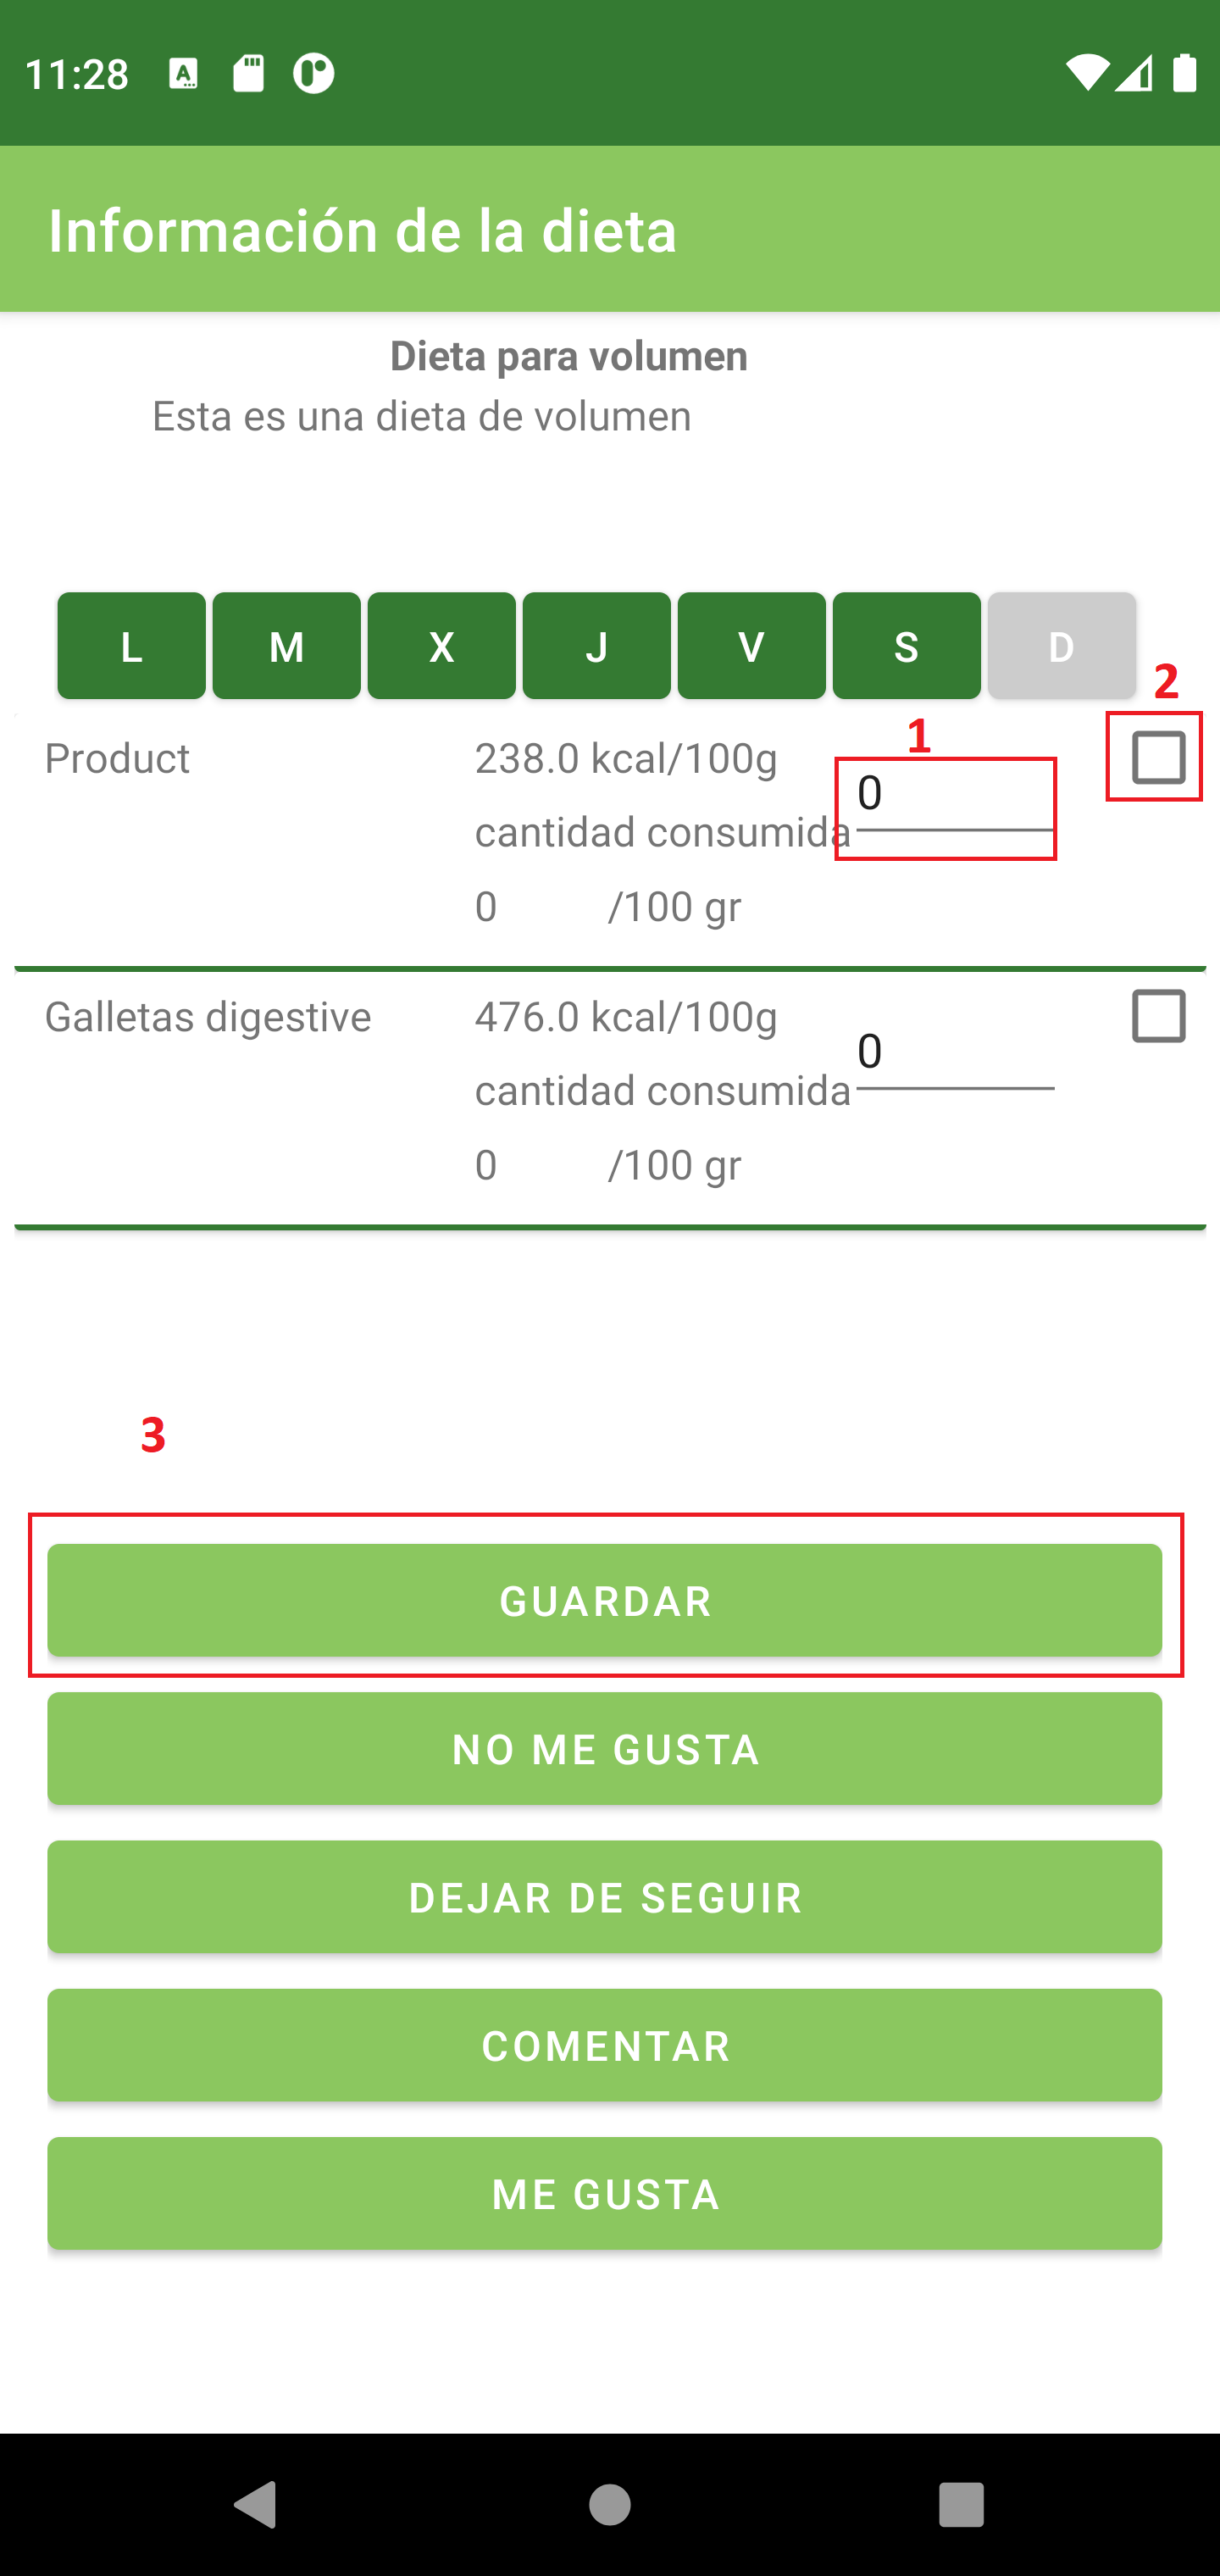
\includegraphics[width=0.5\textwidth]{Images/Capitulo7/modinfodieta.png}
    \caption{Vista de información de dieta con los pasos para actualizar gramos consumidos}
    \label{fig:modinfodieta}
\end{figure}

\begin{figure}[H]
    \centering
    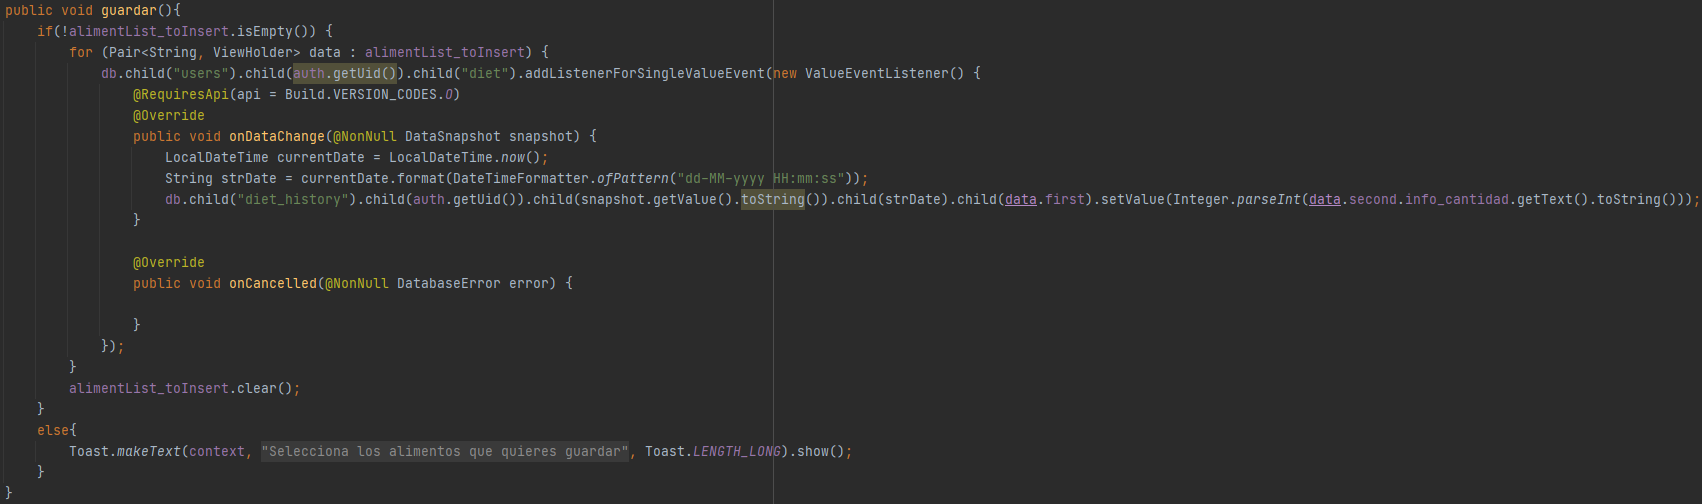
\includegraphics[width=\textwidth]{Images/Capitulo7/savedieta.png}
    \caption{Código del método \texttt{guardar()} que almacena los cambios en la base de datos}
    \label{fig:savedieta}
\end{figure}

En el método de guardar se insertan en la tabla de ``\texttt{diet\_history}`` los alimentos que han sido guardados previamente en la lista de pares, añadiendo una nueva entrada en la base de datos con la fecha actual, con el código del alimento como clave y la cantidad de gramos del alimento consumido como valor.

\subsection{Añadir comentarios}
Esta funcionalidad se creó para que las dietas tuvieran opiniones de los deportistas que se habían suscrito a esa dieta y la habían realizado durante un tiempo. Esta utilidad sirve para conocer cómo otros usuarios han llevado a cabo la dieta, ver si han obtenido los resultados esperados, así cómo comentar las posibles mejoras de la dieta.

Solo los deportistas que siguen la dieta pueden comentar sobre ella, así como los administradores de la aplicación. Los comentarios se realizan sobre la vista de dieta seguida.

En esta vista (ver figura \ref{fig:infodieta}) si se pulsa sobre el botón de comentar, aparecen todos los comentarios de esta dieta así como la posibilidad de escribir un nuevo comentario para la dieta (ver figura \ref{fig:comments}).

\begin{figure}[H]
    \centering
    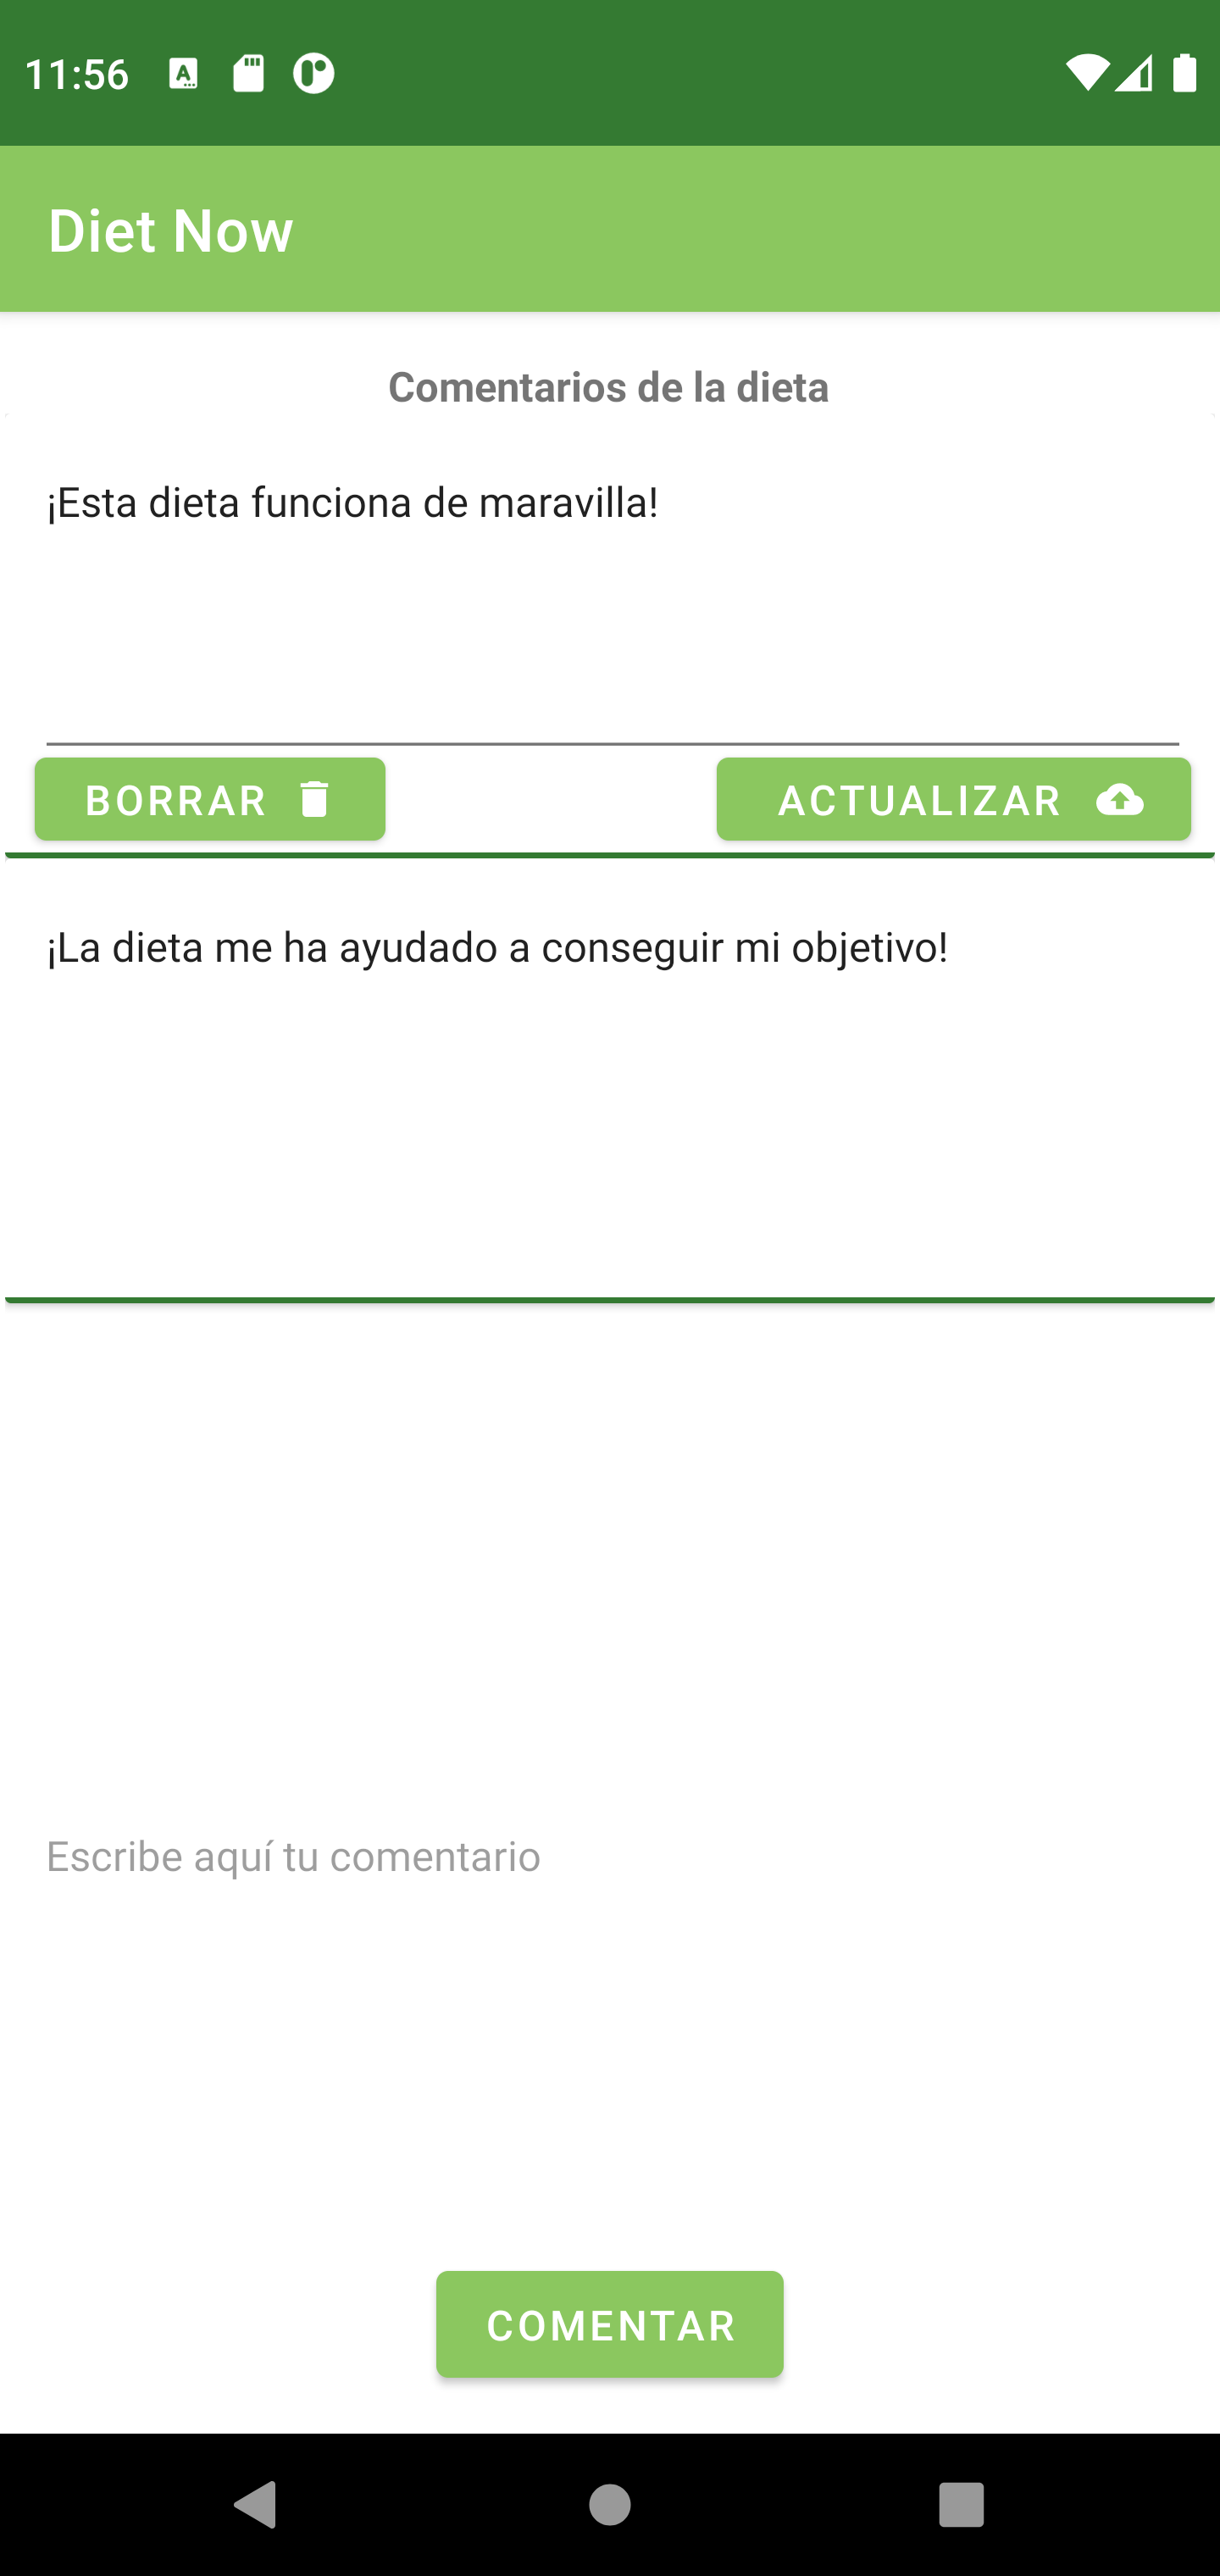
\includegraphics[width=0.4\textwidth]{Images/Capitulo7/comments.png}
        \caption{Vista del módulo comentarios}
    \label{fig:comments}
\end{figure}

Para realizar esta funcionalidad se hace un \texttt{Intent}, redireccionando al usuario a la vista de los comentarios (ver figura \ref{fig:commentcode}).

\begin{figure}[H]
    \centering
    \includegraphics[width=\textwidth]{Images/Capitulo7/commentcode.png}
        \caption{Código del método \texttt{comment()} que redirige a la vista de los comentarios}
    \label{fig:commentcode}
\end{figure}

En este \texttt{Intent} además, se le pasa por parámetro a la vista el id de la dieta mediante el método \texttt{intent.putExtra(“did”,dietId)}, para que en la vista de comentarios ya se tenga guardado el id de la dieta sin necesidad de consultar la base de datos.
En el método \texttt{OnCreate()}  de la actividad \texttt{DietComments}, se guarda en una variable el id de la dieta para ser utilizado posteriormente al insertar comentarios en esa dieta (ver figura \ref{fig:dietcomments}).

\begin{figure}[H]
    \centering
    \includegraphics[width=\textwidth]{Images/Capitulo7/dietcomments.png}
        \caption{Código de la clase \texttt{DietComments()}}
    \label{fig:dietcomments}
\end{figure}

Mediante el método ``\texttt{getIntent().getExtras().getString(“did”)}``, guarda en una variable el id de la dieta. En el caso de que se le hubieran pasado más parámetros a la actividad, solo habría que cambiar el string con el que se hace ``\texttt{intent.putExtra()}`` y el string referenciado en la actividad que recibe los argumentos por medio del \texttt{Intent}.

En la vista de comentarios (ver figura \ref{fig:comments}) se pueden realizar varias acciones:
\begin{enumerate}
    \item Se puede escribir un nuevo comentario sobre la dieta.
    \item Se puede actualizar un comentario previamente realizado por el usuario \textit{logueado} en la aplicación.
    \item Se pueden borrar comentarios previamente realizados por el usuario \textit{logueado} en la aplicación.
\end{enumerate}

Para implementar las funcionalidades descritas anteriormente en la actividad \texttt{DietComments}, en el método \texttt{OnCreate()} de la actividad se llama al método \texttt{getComments()} que carga de base de datos los comentarios de la dieta (ver figura \ref{fig:getcomments}).

\begin{figure}[H]
    \centering
    \includegraphics[width=\textwidth]{Images/Capitulo7/getcomments.png}
    \caption{Código del \texttt{getComments()}}
    \label{fig:getcomments}
\end{figure}

En la tabla comentarios, se recorren todos los comentarios relativos a la dieta actual para posteriormente ir insertándose en una lista, que posteriormente utilizará el adaptador \texttt{CommentsAdapter} para mostrar dinámicamente los distintos comentarios de la dieta.

En el método \texttt{OnBindViewHolder()} del adaptador \texttt{CommentsAdapter} se cargan los datos relativos a cada uno de los comentarios de la dieta, para poder ser visualizados posteriormente por el usuario (ver figura \ref{fig:commentsadapter}).

\begin{figure}[H]
    \centering
    \includegraphics[width=\textwidth]{Images/Capitulo7/commentsadapter.png}
    \caption{Código del método \texttt{OnBindViewHolder()} del adaptador \texttt{CommentsAdapter}}
    \label{fig:commentsadapter}
\end{figure}

En el caso de que el usuario quiera insertar un comentario en la dieta, se insertará en comentario en la base de datos con el método \texttt{uploadComment()} (ver figura \ref{fig:upload_comment_method}).
\begin{figure}[H]
    \centering
    \includegraphics[width=\textwidth]{Images/Capitulo7/uploadcomment.png}
    \caption{Código del método \texttt{uploadComment()}}
    \label{fig:upload_comment_method}
\end{figure}

Las acciones para borrar y actualizar comentarios previamente realizados, se realizan en el \texttt{CommentsAdapter} ya que este contiene la información relativa a cada comentario, así como los botones de actualizar y guardar de cada comentario.
En el caso de querer actualizar el comentario se realizará tras haber cambiado el texto del comentario después de haber pulsado el botón de actualizar relativo al comentario (ver figura \ref{fig:editdelete}).
En el caso de querer borrar el comentario, la actualización se llevará a cabo después de pulsar sobre el botón de borrar el comentario (ver figura \ref{fig:editdelete}).

\begin{figure}[H]
    \centering
    \includegraphics[width=\textwidth]{Images/Capitulo7/editdelete.png}
    \caption{Código de los métodos asociados a editar y borrar comentario}
    \label{fig:editdelete}
\end{figure}

Cada vez que un comentario es actualizado, insertado o borrado, la vista de los comentarios se actualiza, esto es posible ya que en la actividad \texttt{DietComments} se establece un objeto de escucha con el método \texttt{addValueEventListener()} sobre la tabla comentarios, para que cuando se modifique una referencia de esa tabla, actualice la información relativa a la vista (ver figura \ref{fig:getcomments}).

\subsection{Perfil del usuario}
Esta vista ofrece la posibilidad de visualizar información acerca del usuario que ha iniciado sesión en la aplicación así como modificar los datos del perfil. 
Independientemente del rol que tenga el usuario, en el menú principal existe un botón llamado ``Mi Perfil`` que redirige al perfil del usuario que ha iniciado sesión (ver figura \ref{fig:udashboard}).

El módulo perfil de usuario contiene los datos personales del usuario, las gráficas asociadas a su actividad y opciones de administración de cuenta cómo editar o eliminar la cuenta o cerrar sesión.

La ventana de perfil de usuario se puede dividir en las siguientes partes (ver figura \ref{fig:perfedit}):

\begin{itemize}
    \item \textbf{Información personal:} corresponde a la parte superior de la pantalla, en esta parte se muestran  los datos personales del usuario como el nombre, apellido, edad, email, la fecha desde la cual es miembro en la aplicación y la imagen de perfil, además de 2 botones, uno para cambiar la imagen de perfil y otro para ver la gráfica que la dieta actual.
    \item \textbf{Gráficas de pesos y pasos:} mediante el botón deslizante podemos activar las gráficas de pesos y pasos que muestran la evolución de en el tiempo de estos dos registros. El botón circular con el signo “+” permite añadir pasos y/o pesos para el día actual.
    \item \textbf{Acciones:} pulsando sobre el botón de ajustes (imagen de 3 puntos verticales) se despliega un selector con las siguientes opciones:
        \begin{itemize}
        \item \textbf{Historial de dietas:} despliega una nueva ventana donde se muestran por orden cronológico las dietas que ha ido siguiendo el usuario y la dieta que sigue actualmente, al lado de cada dieta hay un botón que para abrir el detalle de la dieta en cuestión.
        \item \textbf{Cerrar sesión:} cierra la sesión del usuario y vuelve a la pantalla de login.
        \item \textbf{Editar perfil:} despliega una nueva ventana donde se pueden editar la información personal del usuario.
        \item \textbf{Eliminar perfil:} despliega una ventana emergente avisando que la eliminación del perfil no se puede deshacer, si el usuario accede se elimina el perfil.
        \end{itemize}
\end{itemize}

\begin{figure}[H]
    \centering
    \includegraphics[width=0.5\textwidth]{Images/Capitulo7/perfedit.png}
        \caption{Vista de Mi Perfil dividida en 3 secciones}
    \label{fig:perfedit}
\end{figure}

A nivel de código, esta ventana se crea con el método \texttt{onCreate()} de ``\texttt{UserProfileActivity}`` (ver figura \ref{fig:userprofileactivity}) Dentro de \texttt{onCreate()} también se declaran todos los listeners de los botones como por ejemplo el de añadir pesos y/o pasos (ver figura \ref{fig:selectorperf}).

\begin{figure}[H]
    \centering
    \includegraphics[width=\textwidth]{Images/Capitulo7/userprofileactivity.png}
        \caption{Código de ``\texttt{UserProfileActivity}``}
    \label{fig:userprofileactivity}
\end{figure}

\begin{figure}[H]
    \centering
    \includegraphics[width=0.5\textwidth]{Images/Capitulo7/selectorperf.png}
    \caption{Selector de pasos o pesos}
    \label{fig:selectorperf}
\end{figure}

Dependiendo de lo que haya elegido el usuario se llama a \texttt{AddStep()} o \texttt{AddWeight()} que se encargan de registrar el valor introducido por el usuario e insertarlo en la base de datos junto con la fecha actual (ver figura \ref{fig:addstep}).

El funcionamiento del resto de los botones en esta vista es similar, se declara el listener que permanece activo a la espera de la ejecución de dicho evento.

\begin{figure}[H]
    \centering
    \includegraphics[width=\textwidth]{Images/Capitulo7/addstep.png}
    \caption{Código del método \texttt{AddStep()}}
    \label{fig:addstep}
\end{figure}

El código de las secciones anteriormente mencionadas es el siguiente:

\begin{itemize}
    \item \textbf{Información personal:} para mostrar la información del usuario, en el \texttt{onCreate()} de la actividad el siguiente código se encarga de hacer la consulta a la base de datos y rellenar los campos (ver figura \ref{fig:consulta}).
\end{itemize}
\begin{figure}[H]
    \centering
    \includegraphics[width=\textwidth]{Images/Capitulo7/consulta.png}
    \caption{Consulta que obtiene la información personal de un usuario}
    \label{fig:consulta}
\end{figure}

El botón ``Cambiar imagen`` abre la galería y cuando un usuario selecciona una imagen, esta se sube a Firebase Storage y se asocia a su perfil (ver figura \ref{fig:getimagephtone}).
\begin{figure}[H]
    \centering
    \includegraphics[width=\textwidth]{Images/Capitulo7/getimagephtone.png}
    \caption{Código que abre la galería del dispositivo}
    \label{fig:getimagephtone}
\end{figure}

El botón ``Gráfico de la dieta actual`` abre una nueva ventana que muestra el gráfico (ver figura \ref{fig:getimagephtone}).

\begin{figure}[H]
    \centering
    \includegraphics[width=0.5\textwidth]{Images/Capitulo7/grafdietact.png}
    \caption{Vista de Gráfico de la dieta actual}
    \label{fig:grafdietact}
\end{figure}

\begin{itemize}
    \item \textbf{Gráficas de pesos y pasos:} en esta sección el usuario dispone de un botón deslizable que activa las dos gráficas disponibles, la de pesos y la de pasos para que pueda visualizarlas. El botón en cuestión se compone de dos partes, un círculo (ver figura \ref{fig:circulo}) que al pulsar se mueve de derecha a izquierda y viceversa con una animación de desplazamiento y un fondo (ver figura \ref{fig:rectangulo}) que cambia de color blanco a verde y viceversa (ver figura \ref{fig:layoutselector}).
\end{itemize}

\begin{figure}[H]
    \centering
    \includegraphics[width=\textwidth]{Images/Capitulo7/layoutselector.png}
    \caption{Layout del botón selector}
    \label{fig:layoutselector}
\end{figure}
\begin{figure}[H]
    \centering
    \includegraphics[width=\textwidth]{Images/Capitulo7/circulo.png}
    \caption{Diseño del thumb del botón selector}
    \label{fig:circulo}
\end{figure}
\begin{figure}[H]
    \centering
    \includegraphics[width=\textwidth]{Images/Capitulo7/rectangulo.png}
    \caption{Diseño del track del botón selector}
    \label{fig:rectangulo}
\end{figure}

Al hacer clic sobre el botón se ejecuta el código asociado a el, que en función de si está a ``\texttt{true}`` o ``\texttt{false}`` activa una gráfica u otra (ver figura \ref{fig:selectorcode}). 
\begin{figure}[H]
    \centering
    \includegraphics[width=\textwidth]{Images/Capitulo7/selectorcode.png}
    \caption{Código del botón selector de gráfica}
    \label{fig:selectorcode}
\end{figure}

Para las gráficas de la aplicación se ha utilizado la librería de AnyChart \cite{anychart}. Ambas gráficas tienen una implementación similar ya que su almacenamiento en la base de datos es similar de modo que lo único que cambia es la tabla donde están los datos pero el formato y la renderización de estos es idéntica. En la figura \ref{fig:stepschart} se puede ver cómo está implementada la gráfica de pasos.
\begin{figure}[H]
    \centering
    \includegraphics[width=\textwidth]{Images/Capitulo7/stepschart.png}
    \caption{Código del gráfico de pasos}
    \label{fig:stepschart}
\end{figure}
    
\begin{itemize}
    \item \textbf{Acciones:} si el usuario presiona en el botón con 3 puntos verticales se le desplegará un menú con 4 opciones (ver figura \ref{fig:opt}), cada opción tiene asociada su función en el código (ver figura \ref{fig:optcode}):
\end{itemize}    

\begin{figure}[H]
    \centering
    \includegraphics[width=0.5\textwidth]{Images/Capitulo7/opt.png}
    \caption{Vista ``Mi Perfil`` con la lista de acciones desplegada}
    \label{fig:opt}
\end{figure}
\begin{figure}[H]
    \centering
    \includegraphics[width=\textwidth]{Images/Capitulo7/optcode.png}
    \caption{Código de la lista de acciones}
    \label{fig:optcode}
\end{figure}
    
\begin{itemize}
    \begin{itemize}
        \item \textbf{Historial de dietas:} al seleccionarlo se abre la vista Historial de dietas (ver figura \ref{fig:historialdietas}). El método \texttt{DietHistory()} se encarga de obtener la lista de dietas de la base de datos y de mostrar la vista (ver figura \ref{fig:diethistory}).
    \end{itemize}
\end{itemize}    
\begin{figure}[H]
    \centering
    \includegraphics[width=0.5\textwidth]{Images/Capitulo7/historialdietas.png}
    \caption{Vista Histórico de dietas}
    \label{fig:historialdietas}
\end{figure}
\begin{figure}[H]
    \centering
    \includegraphics[width=\textwidth]{Images/Capitulo7/diethistory.png}
    \caption{Código del método \texttt{DietHistory()} que genera la vista Histórico de dietas}
    \label{fig:diethistory}
\end{figure}
    
    
\begin{itemize}    
    \begin{itemize}
        \item \textbf{Cerrar sesión:} cierra la sesión del usuario y vuelve la pantalla de inicio de sesión (ver figura \ref{fig:logout}).
    \end{itemize}
\end{itemize}
\begin{figure}[H]
    \centering
    \includegraphics[width=\textwidth]{Images/Capitulo7/logout.png}
    \caption{Código del método \texttt{logout()} que genera cierra sesión y redirige al login}
    \label{fig:logout}
\end{figure}

\begin{itemize}    
    \begin{itemize}
        \item \textbf{Editar perfil:} abre la vista de edición de perfil (ver figura \ref{fig:editarperf}). El método \texttt{editProfile()} se encarga de crear la nueva vista (ver figura \ref{fig:editprofilecode}).
    \end{itemize}
\end{itemize}

\begin{figure}[H]
    \centering
    \includegraphics[width=0.5\textwidth]{Images/Capitulo7/editarperf.png}
    \caption{Vista de editar perfil}
    \label{fig:editarperf}
\end{figure}
\begin{figure}[H]
    \centering
    \includegraphics[width=\textwidth]{Images/Capitulo7/editprofilecode.png}
    \caption{Código del método \texttt{editProfile()}}
    \label{fig:editprofilecode}
\end{figure}

\begin{itemize}    
    \begin{itemize}
        \item \textbf{Eliminar perfil:} deshabilita el perfil en la base de datos y vuelve a la pantalla de inicio (ver figura \ref{fig:delete}).
    \end{itemize}
\end{itemize}
\begin{figure}[H]
    \centering
    \includegraphics[width=\textwidth]{Images/Capitulo7/delete.png}
    \caption{Código del método \texttt{delete()} que deshabilita el perfil}
    \label{fig:delete}
\end{figure}






